\documentclass[conference]{IEEEtran}
\IEEEoverridecommandlockouts
\usepackage{amsmath,amssymb,booktabs,array,graphicx,microtype,caption,float}
\usepackage[table]{xcolor}
\usepackage{hyperref}
\hypersetup{
  colorlinks=false,
  pdfborder={0 0 2},
  citebordercolor={0 0.85 0},
  linkbordercolor={1 0 0},
  urlbordercolor={0 0.2 1}
}
\urlstyle{same}
\setlength{\textfloatsep}{7pt plus 2pt minus 2pt}
\setlength{\floatsep}{6pt plus 2pt minus 2pt}
\setlength{\intextsep}{6pt plus 2pt minus 2pt}
\renewcommand{\topfraction}{0.95}
\renewcommand{\bottomfraction}{0.90}
\renewcommand{\textfraction}{0.05}
\renewcommand{\floatpagefraction}{0.80}
\renewcommand{\dbltopfraction}{0.95}
\renewcommand{\dblfloatpagefraction}{0.80}
\setcounter{topnumber}{4}
\setcounter{bottomnumber}{3}
\setcounter{totalnumber}{6}
\setcounter{dbltopnumber}{3}
\makeatletter
\setlength{\@dblfptop}{0pt}
\setlength{\@dblfpbot}{0pt plus 1fil}
\makeatother
\setlength{\parindent}{1em}
\setlength{\parskip}{0pt}
\renewcommand{\arraystretch}{0.98}
\newcommand{\model}{\textsc{CSI2Text-PGMT}}
\newcommand{\los}{\textsc{LoS}}
\newcommand{\nlos}{\textsc{NLoS}}
\definecolor{modelblue}{RGB}{225,239,250}
\definecolor{priorgreen}{RGB}{150,225,150}
\definecolor{gainblue}{RGB}{0,82,155}
\definecolor{gainred}{RGB}{170,0,0}
\definecolor{gainrow}{RGB}{245,245,245}
\newcommand{\best}[1]{\underline{#1}}
\newcommand{\relgain}[1]{\textcolor{gainred}{\bfseries\boldmath #1}}
\newcommand{\relloss}[1]{\textcolor{gainblue}{\bfseries\boldmath #1}}
\newcommand{\priorwork}[1]{#1}

\title{CSI2TEXT-PGMT: Physics-Grounded Multitask Channel Reporting from CSI}
\author{}

\begin{document}
\maketitle

\begin{abstract}
Raw channel state information (CSI) is high-dimensional and complex-valued, making it difficult for
network controllers and operators to directly interpret, retrieve and reuse. Future autonomous
wireless networks require not only channel state estimation but also the understanding of underlying
physical propagation mechanisms. Although existing unconstrained language decoders can generate
fluent reports, their outputs may violate physical facts. To address this issue, this paper proposes
CSI2TEXT-PGMT, a physics-prior-constrained multi-task framework that transforms heterogeneous
beam-frequency CSI into structured and verifiable channel descriptions. The
system-configuration-aware Transformer encoder learns shared CSI representations via semantic
alignment with textual descriptions and propagation prototypes. Multiple task-specific branches
estimate propagation attributes concerning delay, angle, power and multipath structure. A relation
correction module enforces physical dependencies among diverse predictions, while a deterministic
language generation module produces final channel analysis reports. Extensive experiments verify
that the framework accurately recovers various propagation attributes, distinguishes LoS/NLoS
scenarios, reduces logical inconsistencies among joint physical predictions, and generates physically
faithful descriptions. Furthermore, learned representations are evaluated on downstream tasks
including adaptive beam search, MCS link adaptation and link quality/outage prediction, which
demonstrates the framework's capability for physical channel interpretation and effective support for
wireless resource management decisions.
\end{abstract}

\begin{IEEEkeywords}
Channel state information, channel reporting, physics-grounded learning, wireless intelligence,
multitask learning.
\end{IEEEkeywords}

\section{Introduction}

Autonomous wireless networks require more than accurate channel-state estimation; they also need
interpretable knowledge of the underlying propagation conditions, including whether a link is LoS
or NLoS, which path dominates, how severe the delay and angular dispersion are, and whether
reflection-rich propagation may impair beam management or positioning. However, raw CSI does not
directly provide such an interface: conventional estimators return fragmented physical attributes,
whereas unconstrained language decoders may produce plausible descriptions that are not supported
by the measured channel.

Recent studies have made important progress in learning representations from wireless channels and
connecting wireless signals with language. Channel charting recovers geometry-preserving
representations from CSI~\cite{studer2018charting}, while reusable CSI representations support
channel prediction, positioning, and cross-configuration transfer~\cite{liu2024wifo,palhares2025csi2vec}.
More recently, wireless-language models have generated human-action captions from Wi-Fi
CSI~\cite{wei2026wifi2cap}, aligned unsegmented CSI streams with language models for zero-shot
activity understanding~\cite{keya2026wirelesssense}, and introduced an RF-language model for waveform
and spectrum understanding~\cite{zou2026rfgpt}.
These methods demonstrate the potential of wireless-language modeling, but they primarily describe
human activities or communication-signal content rather than the propagation channel itself.
Meanwhile, existing CSI models usually output latent embeddings, reconstructed channels, locations,
or selected physical parameters, leaving propagation information fragmented and inaccessible as a
unified channel report.

This separation reveals a fundamental challenge. CSI-to-language conversion requires a model to
first recover a coherent physical record and then express that record in natural language. The first
stage determines whether quantities such as delay, angle, power, and path count are supported by the
CSI, whereas the second determines whether they are presented completely and readably. Assigning
both responsibilities to an unconstrained language decoder can produce fluent and structurally
plausible descriptions without guaranteeing numerical accuracy or physical consistency. For
propagation-aware network operation, such errors are critical because a well-written but incorrect
channel report may directly mislead downstream decisions.

In this work, we take a different perspective: rather than asking a large language model to freely
interpret CSI, we formulate CSI-to-text conversion as physics-grounded structured inference followed
by faithful verbalization. We propose CSI2Text-PGMT, a configuration-aware multitask framework that
transforms beam-frequency CSI into an auditable channel description. A shared Transformer encoder
processes phase-aligned and beamspace-transformed complex CSI while conditioning its representation
on the acquisition configuration. Contrastive objectives further align CSI samples with instance
descriptions and coarse propagation prototypes.

Target-specific branches recover heterogeneous physical attributes using delay-domain features for
temporal quantities, raw-amplitude statistics for power-related attributes, circular representations for
angles, and coarse-to-fine estimation for continuous targets. Before verbalization, a lightweight
relational correction module removes impossible values and reconciles known dependencies among the
predicted attributes. A deterministic verbalizer then converts the corrected record into natural
language while suppressing inapplicable fields. Consequently, every reported category and numerical
value can be traced to an explicit physical prediction rather than being freely generated by a language
model.

We evaluate CSI2Text-PGMT on a LoS-balanced dataset containing 50,000 samples and compare it
with conventional neural baselines and four direct CSI-to-text decoders based on Qwen3-1.7B,
Qwen3.5-2B, InternLM3-8B, and DeepSeek-R1-Qwen3-8B. The proposed model achieves a
first-path-delay mean absolute error of 21.91 ns and produces channel reports with 96.43\% composite
factuality. Although the direct language decoders generate fluent and nearly complete records, their
delay-slot tolerance accuracy ranges from only 17.81\% to 28.33\%, compared with 96.05\% for our
structured pipeline. The framework also maintains high description factuality under unseen frequency
and array configurations, demonstrating that its advantage is not limited to a single acquisition setting.
Further robustness and stratified analyses identify NLoS first-path inference as the main remaining
failure mode, revealing a concrete direction for future multipath-aware modeling and uncertainty
calibration.

To further assess practical utility, we add five downstream wireless-control tasks. The learned
interface gives a 34.15 m mean localization error with 49.02\% of links within 10 m, reaches
70.92\% accuracy for adaptive cyclic-prefix selection, and estimates link quality with a 2.1098 dB
power MAE while retaining 98.92\% outage accuracy. For resource-management decisions, it achieves
99.05\% MCS accuracy with only 0.53\% BLER violations and 99.90\% oracle goodput, and obtains
87.84\% Top-1 and 96.52\% Top-3 accuracy for 64-beam transmit-beam search with only 1.33 dB mean
gain loss.

Our \textbf{main contributions} are summarized as follows:
\begin{enumerate}
\renewcommand{\labelenumi}{\roman{enumi}.}
\item We formulate CSI-to-language conversion as physics-grounded structured inference followed by
faithful verbalization, separating physical correctness from linguistic plausibility.
\item We propose CSI2TEXT-PGMT, a configuration-aware multitask architecture that combines
semantic alignment, target-specific physical branches, relational correction, and deterministic
verbalization to produce traceable channel reports.
\item We demonstrate that structured prediction grounds channel descriptions substantially more
accurately than direct learned decoding, and use cross-configuration, robustness, and stratified
evaluations to identify NLoS multipath inference as the dominant remaining challenge.
\end{enumerate}
The code is available at \url{https://github.com/yanrunhui/CSI_clip_model}.

\section{Preliminaries}

\paragraph{Multipath CSI and delay observability.}
After retaining one receive element, the frequency-domain CSI is represented by a complex matrix
$\mathbf H$ across transmit antennas and subcarriers. Under a multipath model,
\[
H_{m,k}=\sum_{p=1}^{P} \alpha_p a_m(\phi_p)e^{-j2\pi f_k\tau_p}+n_{m,k},
\]
Here, $m\in\{1,\ldots,N_{\mathrm{tx}}\}$, $k\in\{1,\ldots,N_f\}$, and
$p\in\{1,\ldots,P\}$ index the transmit antenna element, subcarrier, and propagation path,
respectively, where $P$ is the number of retained paths. Moreover, $\alpha_p$, $\tau_p$, and
$\phi_p$ denote the complex gain, delay, and transmit-side direction of path $p$; $f_k$ is the
$k$-th subcarrier frequency; $a_m(\phi_p)$ is the corresponding transmit-array response at antenna
$m$; and $n_{m,k}$ is complex measurement noise. Thus, spatial information is encoded across the
transmit-array dimension, while delay is encoded by phase variation across frequency. For a dominant
path, adjacent subcarriers satisfy
\[
H_{m,k+1}H_{m,k}^{*}\propto e^{-j2\pi\Delta f\tau}.
\]
The superscript $(\cdot)^*$ denotes complex conjugation, and
$\Delta f=f_{k+1}-f_k$ is the adjacent-subcarrier spacing. This relation shows that propagation
delay can be inferred from frequency-dependent phase. Its resolution depends on the observed
bandwidth and subcarrier spacing, motivating the use of acquisition configuration in the model.
Under multipath propagation, overlapping components make a single closed-form estimate insufficient.

\paragraph{Beam-delay representation and AoA observability.}
We expose the spatial and temporal structures using the beam-delay power representation
\[
\mathbf P_{\mathrm{bd}}=
\left|\operatorname{IFFT}_{f}\!\left(\operatorname{FFT}_{\mathrm{array}}(\mathbf H)\right)\right|^2.
\]
Here, $\mathbf P_{\mathrm{bd}}$ denotes the beam-delay power representation obtained by applying a
spatial FFT over the transmit array, an IFFT over frequency, and an element-wise magnitude square.
A propagation path ideally produces concentrated energy in this domain, motivating our beam tokens
and delay-specific branches. The retained spatial aperture is on the transmit side,
whereas the supervised target is receiver-side AoA. Because only one receive element is retained,
classical receive-array estimators cannot directly recover this angle. The model therefore learns
receiver-side AoA from the statistical relationship between transmit-side beam-frequency CSI,
multipath structure, and ray-traced geometry. Accordingly, AoA is treated as a supervised
cross-domain prediction target rather than a directly measured beam direction.

\section{Method}

CrossConfig-CSI converts heterogeneous CSI $\mathbf H$ and acquisition configuration $\mathbf c$
into a structured record and an auditable report:
\[
\hat{\mathbf y}=f_{\Theta}(\mathbf H,\mathbf c),
\qquad
\hat{s}=V\!\left(\mathcal C(\hat{\mathbf y})\right),
\]
where $\mathcal C$ corrects known relations and $V$ deterministically verbalizes the resulting record.

\begin{figure}[!t]
\centering
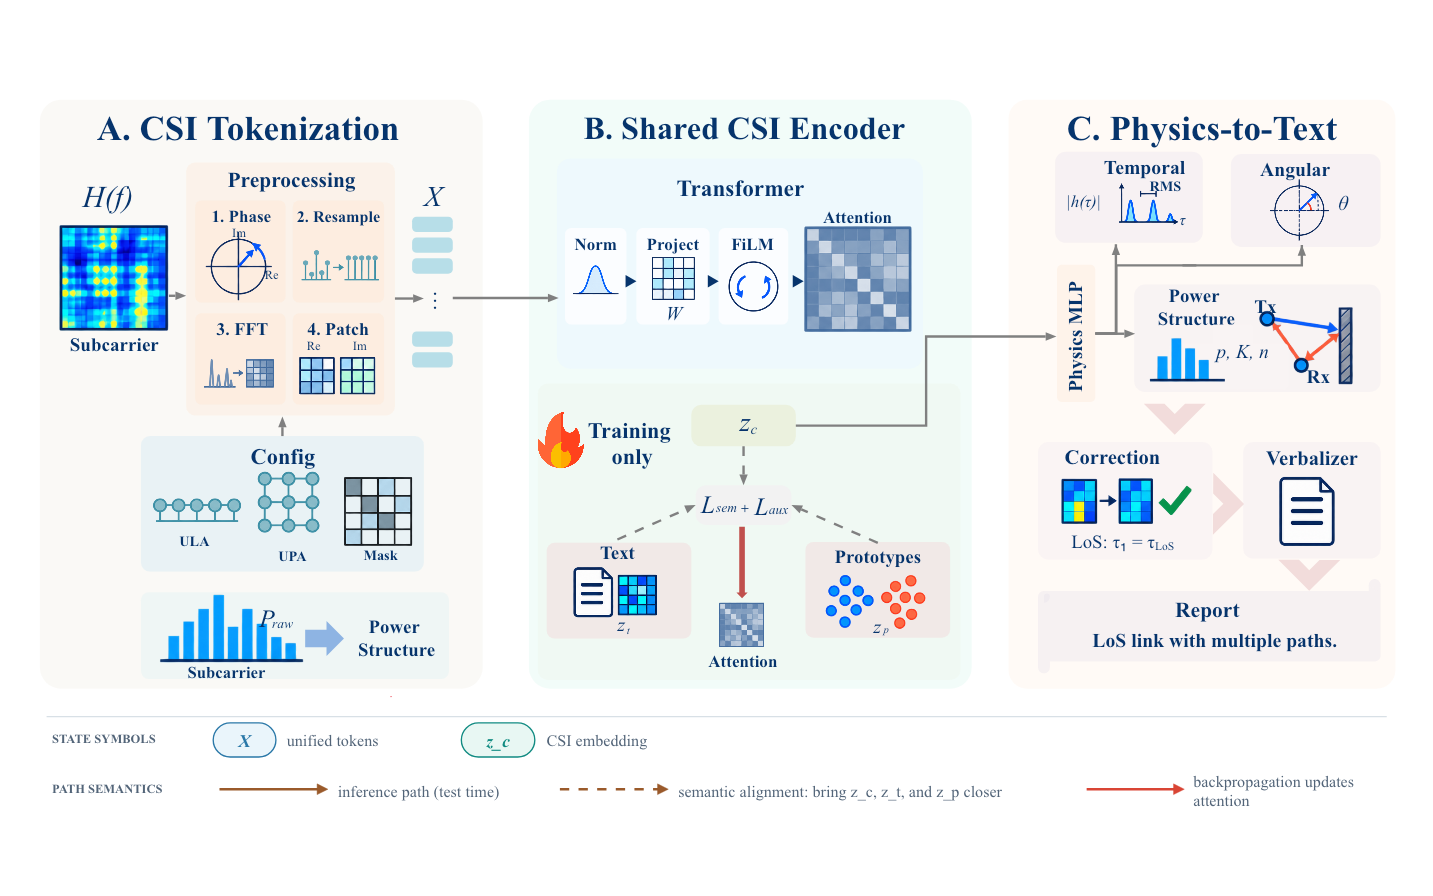
\includegraphics[width=0.98\columnwidth]{figures/CSI2TEXT-PGMT-16x10-labeled.png}
\caption{Overview of \model{}. Stage A phase-aligns, frequency-resamples, and transforms the
heterogeneous CSI into unified beam-frequency tokens while retaining a raw-power bypass. Stage B
uses configuration conditioning and a shared Transformer encoder; text and prototype embeddings
provide semantic supervision only during training. Stage C maps the shared CSI embedding to temporal,
angular, and power/structure predictions, applies relational correction, and deterministically verbalizes
the corrected physical record. Solid arrows denote the test-time inference path, dashed arrows denote
training-only semantic alignment, and the red arrow shows the backpropagation update to attention.}
\label{fig:method-overview}
\end{figure}

Section~III-A unifies heterogeneous CSI through phase alignment, frequency resampling, and beamspace
tokenization. Section~III-B learns a configuration-conditioned shared representation with training-only
text and prototype alignment. Section~III-C predicts temporal, angular, power, and multipath fields with
structure-matched branches. Section~III-D corrects known relations and deterministically verbalizes the
record, completing a traceable CSI-to-report pipeline.

\subsection{Unified CSI Tokenization}

Consider frequency-domain CSI
\[
\mathbf H\in\mathbb C^{N_{\mathrm{rx}}\times N_{\mathrm{tx}}\times N_f}.
\]
Because its dimensions vary with array geometry and frequency sampling, we transform each observation into
\[
(\mathbf X,\mathbf M,\mathbf B)=\mathcal T(\mathbf H,\mathbf c),
\]
where $\mathbf X$ is the unified token tensor, $\mathbf M$ its validity mask, and $\mathbf B$ the
normalized beam positions.

We remove arbitrary global phase using a reference coefficient,
\[
\mathbf H^{(a)}=\mathbf H\exp\!\left(-j\angle H_{\mathrm{ref}}\right).
\]
and resample through the delay domain to a fixed $N_f^\star$ before the beamspace transform
\[
\mathbf H_{\mathrm{beam}}=
\begin{cases}
\operatorname{FFT}_{\mathrm{ant}}(\mathbf H^{(a)}),&\text{ULA},\\
\operatorname{FFT2}_{\mathrm{row,col}}(\mathbf H^{(a)}),&\text{UPA}.
\end{cases}
\]
Adjacent ULA beams or local UPA beam patches form tokens by concatenating real and imaginary
components; $\mathbf M$ excludes padded boundaries.

\subsection{Configuration-Aware Representation Learning}

The valid elements of each example are standardized before entering the shared encoder:
\[
\widetilde{\mathbf X}=
\frac{\mathbf X-\mu_{\mathbf X}}{\sigma_{\mathbf X}+\epsilon},
\]
where the mean and standard deviation are computed only over tokens selected by $\mathbf M$.
This removes link-dependent scale variation.

Each token is projected with linear, depthwise-pointwise convolutional, and adaptive-pooling layers.
Subcarrier spacing modulates the result through
\[
\operatorname{FiLM}(\mathbf u;\Delta f)=
\left(1+\boldsymbol{\gamma}(\Delta f)\right)\odot\mathbf u+
\boldsymbol{\beta}(\Delta f).
\]
Beam-position and configuration encodings are then added. A shared Transformer fuses a learned
$[\mathrm{CLS}]$ token with the masked token mean:
\[
\mathbf z_c=\operatorname{Norm}\!\left[
\mathcal P_c\!\left(\mathbf Z_{\mathrm{cls}}+
\frac{\sum_k M_k\mathbf Z_k}{\sum_k M_k}\right)\right].
\]

\paragraph{Training-only semantic alignment.}
During training, a text encoder maps description $s_i$ to $\mathbf z_t^i$, and a prototype bank maps
coarse semantic key $k_i$ to $\mathbf z_p^i$:
\[
\mathbf z_t^i=f_{\mathrm{text}}(s_i),
\qquad
\mathbf z_p^i=\mathbf P(k_i).
\]
The key summarizes environment, LoS/NLoS state, path richness, and coarse physical regimes. We use
symmetric contrastive alignment:
\[
\mathcal L_{\mathrm{align}}=
\mathcal L_{\mathrm{NCE}}(\mathbf z_c,\mathbf z_t)+
\mathcal L_{\mathrm{NCE}}(\mathbf z_c,\mathbf z_p)+
\mathcal L_{\mathrm{NCE}}(\mathbf z_t,\mathbf z_p).
\]
Semantic and balanced $K$-factor-bin classifiers add supervision; all text/prototype branches are
removed at inference.

\subsection{Physics-Aware Structured Prediction}

A residual MLP first maps the shared embedding to a physics-oriented representation:
\[
\mathbf z_{\mathrm{phy}}=\mathbf z_c+\alpha g_{\mathrm{shared}}(\mathbf z_c).
\]
Target-specific branches predict categorical, temporal, angular, power, and multipath fields. The
temporal branch combines $\mathbf z_{\mathrm{phy}}$ with delay-domain features and uses coarse-bin
classification followed by within-bin regression:
\[
\hat y=l_{\hat b}+\hat r\left(u_{\hat b}-l_{\hat b}\right),
\]
where $\hat b$ is the interval, $\hat r$ its normalized position, and $l_{\hat b},u_{\hat b}$ its bounds.

The angular branch uses sine/cosine outputs to respect periodicity:
\[
\hat\theta=\operatorname{atan2}(\hat s_\theta,\hat c_\theta).
\]

\paragraph{Raw-scale power bypass.}
Because standardization removes absolute amplitude, unstandardized tokens provide a raw-scale feature:
\[
\mathbf r_{\mathrm{raw}}=g_{\mathrm{raw}}(\mathbf X,\mathbf M).
\]
The power head combines it with the shared physics representation:
\[
\hat p_1=g_{\mathrm{power}}\!\left([\mathbf z_{\mathrm{phy}};\mathbf r_{\mathrm{raw}}]\right).
\]
Let $\mathcal Q$ denote the set of physical targets. The overall training objective is
\[
\mathcal L=\sum_{q\in\mathcal Q}\lambda_q\mathcal L_q+
\lambda_{\mathrm{align}}\mathcal L_{\mathrm{align}}+
\lambda_{\mathrm{sem}}\mathcal L_{\mathrm{sem}}+
\lambda_{\mathrm{attr}}\mathcal L_{\mathrm{attr}},
\]
where $\mathcal L_q$ matches the target type; weights and intervals are detailed in the appendix.

\subsection{Relational Correction and Verbalization}

Specialized heads may violate simple relations, so a deterministic correction precedes text generation:
\[
\widetilde{\mathbf y}=\mathcal C(\hat{\mathbf y}).
\]
It clamps invalid negative spreads/counts, enforces at least one path, and equates earliest-path and
direct-LoS delay for predicted LoS samples:
\[
\widetilde{\tau}_1=\widetilde{\tau}_{\mathrm{LoS}}=\hat{\tau}_{\mathrm{LoS}}.
\]
The correction is non-learned. A deterministic verbalizer then produces
\[
\hat{s}=V(\widetilde{\mathbf y}).
\]
Conditional templates suppress inapplicable fields; every emitted value comes from the corrected record.

During inference, the complete path is
\[
(\mathbf H,\mathbf c)\rightarrow\mathbf X\rightarrow\mathbf z_c\rightarrow
\hat{\mathbf y}\rightarrow\widetilde{\mathbf y}\rightarrow\hat{s},
\]
with all semantic supervision removed.

\section{Experiments}

We organize the evaluation around seven questions. Section~IV-A compares physical estimators and
general-purpose language decoders, then examines measured inference cost. Section~IV-B tests
generalization across frequency samplings, antenna arrays, spatial blocks, and unseen maps.
Section~IV-C studies robustness to complex AWGN, Section~IV-D isolates semantic alignment and physical
prediction-head components, and Section~IV-E analyzes the dominant LoS--NLoS failure modes.
Section~IV-F evaluates uncertainty-based selective prediction, while Section~IV-G validates the delay
pipeline on measured SISO data.

\subsection{Main Results: Physical Grounding and CSI-to-Language}

\subsubsection{Comparison with Conventional Physical Estimators}

We first compare \model{} with representative conventional CSI-based physical estimators. The
baselines include PDP/IFFT + MLP, which transforms frequency-domain CSI into delay-domain features
before regression; Flattened CSI + MLP, which directly vectorizes the complex CSI observation; a
Transformer without task-specific branches; a CNN baseline over the beam--frequency input; and a
non-learned IFFT--PDP estimator that reads delay and power statistics from the power-delay profile.
A CSI encoder with single-task heads is also included to isolate the effect of sharing the encoder
while predicting each target independently.

All methods are evaluated on the D2Los\_Data split under the same UPA-$8{\times}8$ setting with
128 CSI frequency points. For each seed, 40,000 training samples are randomly drawn from the source
pool and evaluated on 10,000 held-out samples. LoS and NLoS links are balanced in both training and
test sets to avoid visibility bias, and learned models are trained with three random seeds. As shown
in Figure~\ref{fig:method-overview}, \model{} uses the same CSI observation as input but routes the
shared representation through physics-aware branches before deterministic report generation.

\begin{table}[!t]
\centering
\caption{Main balanced-split physical results. Learned methods report mean $\pm$ sample standard
deviation over three seeds; the deterministic IFFT--PDP baseline is evaluated once on 10,000 test
examples. Lower is better for MAE; higher is better for reflection-bin accuracy. Underlining marks
the best result across all methods, including ours. The final row gives the relative change from the
best prior method, with direction indicated by color (red: improvement; blue: degradation).}
\label{tab:physical-main}
\scriptsize
\setlength{\tabcolsep}{4.0pt}
\resizebox{\columnwidth}{!}{%
\begin{tabular}{lccc}
\toprule
\textbf{Method} & \textbf{Delay (ns) $\downarrow$} & \textbf{Angle ($^\circ$) $\downarrow$} &
\textbf{Power (dB) $\downarrow$} \\
\midrule
\rowcolor{modelblue}\textbf{\model{}} & $\best{\boldsymbol{21.911\!\pm\!0.303}}$ & $\best{\boldsymbol{18.372\!\pm\!0.365}}$ & $\best{\boldsymbol{4.958\!\pm\!0.269}}$ \\
\textbf{CSI encoder + single-task heads} & $51.164\!\pm\!6.248$ & $20.449\!\pm\!0.431$ & $5.074\!\pm\!0.209$ \\
\textbf{PDP/IFFT + MLP} & $28.750\!\pm\!4.611$ & $40.292\!\pm\!0.159$ & $12.236\!\pm\!0.278$ \\
\textbf{Flattened CSI + MLP} & $114.371\!\pm\!0.978$ & $32.782\!\pm\!0.413$ & $13.315\!\pm\!1.221$ \\
\textbf{Transformer without branches} & $145.177\!\pm\!0.003$ & $42.614\!\pm\!0.005$ & $28.091\!\pm\!0.012$ \\
\textbf{CNN baseline} & $169.671\!\pm\!0.021$ & $53.111\!\pm\!0.005$ & $38.090\!\pm\!0.013$ \\
\textbf{IFFT--PDP (non-learned)} & $160.262$ & N/A & $6.555$ \\
\midrule
\rowcolor{gainrow}\textbf{Rel. change vs. best prior} & \relgain{$23.8\%$} & \relgain{$10.2\%$} & \relgain{$2.3\%$} \\
\bottomrule
\end{tabular}}
\vspace{2pt}

\resizebox{\columnwidth}{!}{%
\begin{tabular}{lccc}
\toprule
\textbf{Method} & \textbf{$K$ (dB) $\downarrow$} & \textbf{Refl. MAE $\downarrow$} &
\textbf{Bin acc. $\uparrow$} \\
\midrule
\rowcolor{modelblue}\textbf{\model{}} & $\boldsymbol{1.983\!\pm\!0.263}$ & $\best{\boldsymbol{0.983\!\pm\!0.005}}$ & $\best{\boldsymbol{0.7061\!\pm\!0.0039}}$ \\
\textbf{CSI encoder + single-task heads} & $\best{1.521\!\pm\!0.090}$ & $1.222\!\pm\!0.072$ & $0.5523\!\pm\!0.0259$ \\
\textbf{PDP/IFFT + MLP} & $5.002\!\pm\!0.275$ & $1.706\!\pm\!0.032$ & $0.4420\!\pm\!0.0201$ \\
\textbf{Flattened CSI + MLP} & $5.600\!\pm\!1.013$ & $1.835\!\pm\!0.196$ & $0.4237\!\pm\!0.0999$ \\
\textbf{Transformer without branches} & $20.762\!\pm\!0.051$ & $3.214\!\pm\!0.021$ & $0.1808\!\pm\!0.0008$ \\
\textbf{CNN baseline} & $40.852\!\pm\!0.055$ & $10.134\!\pm\!0.011$ & $0.1562\!\pm\!0.1463$ \\
\textbf{IFFT--PDP (non-learned)} & $20.063^{\ast}$ & N/A & N/A \\
\midrule
\rowcolor{gainrow}\textbf{Rel. change vs. best prior} & \relloss{$30.4\%$} & \relgain{$19.6\%$} & \relgain{$27.8\%$} \\
\bottomrule
\end{tabular}}
\vspace{2pt}

{\scriptsize $^{\ast}$Dominant-to-residual ray-power-ratio heuristic, not a multi-snapshot Rician
estimator. The non-learned baseline additionally obtains path-count MAE 1.6445, delay-spread MAE
36.570 ns, and LoS accuracy 84.72\%. Receiver-side angle and reflection outputs are unavailable
under the single-receive-element observation.}
\end{table}

Table~\ref{tab:physical-main} shows that conventional estimators can fit individual attributes but
struggle to provide a complete and consistent propagation record. The non-learned IFFT--PDP pipeline
is useful for direct delay-domain cues, yet it cannot output receiver-side angle or reflection fields.
Flattened MLP and CNN models are much weaker on delay, angle, power, and multipath quantities because
they do not explicitly preserve the coupled beam--frequency evidence. The generic Transformer has
higher capacity but still lacks the target-matched temporal, angular, power, and structure branches.
By contrast, \model{} obtains the best delay, angle, power, reflection-MAE, and reflection-bin
accuracy, with relative gains of 23.8\%, 10.2\%, 2.3\%, 19.6\%, and 27.8\%, respectively, over the
best prior baseline. The only exception is the scalar $K$-factor result of the single-task baseline,
which indicates that the proposed design is strongest for coupled channel reporting rather than for
every isolated scalar target.

\subsubsection{Comparison with General-Purpose Language Models}

We next compare with direct CSI-to-language baselines built on general-purpose LLMs. Qwen3-1.7B and
Qwen3.5-2B are compact open language models, InternLM3-8B provides a larger instruction-following
backbone, and DeepSeek-R1-Qwen3-8B represents a reasoning-oriented decoder. These models are tested
as direct report generators rather than as post-processing modules for the structured predictions of
\model{}.

The experimental route is CSI $\rightarrow$ CSIEncoder $\rightarrow$ MLP projection $\rightarrow$
continuous prefix embedding $\rightarrow$ LLM $\rightarrow$ physical-attribute JSON and textual
description. The LLM receives continuous vectors learned from CSI, while the prompt supplies the
observation configuration, including array type, bandwidth, and subcarrier spacing, and requires a
fixed output schema. During training, the language-model loss is computed only on the target answer;
tokens corresponding to the CSI prefix and prompt are masked with $-100$ and do not contribute to the
loss. Depending on the run configuration, the CSIEncoder can be trained, frozen, or initialized from
existing weights, while the LLM backbone is frozen and optional LoRA adapters can be trained. The data
split follows the same balanced evaluation protocol as above, with the reported decoder comparison
using the common 1,000-example cohort.

\begin{table}[H]
\centering
\caption{Structured prediction versus direct general-purpose language decoding on the common
1,000-example cohort. Panel A reports description-level quality; Panel B reports field-level error.
Higher is better for accuracy and slot F1; lower is better for hallucination and MAE. Underlining
marks the best result across all methods, including ours. Signed changes are computed against the
best direct decoder; direction is indicated by color (red: improvement; blue: degradation).}
\label{tab:decoder-overall}
\scriptsize
\setlength{\tabcolsep}{4pt}
{\scriptsize\textbf{Panel A: description-level quality}}\par\vspace{1pt}
\resizebox{\columnwidth}{!}{%
\begin{tabular}{lccc}
\toprule
\textbf{Method} & \textbf{Factuality (\%) $\uparrow$} & \textbf{Numeric acc. (\%) $\uparrow$} &
\textbf{Slot F1 (\%) $\uparrow$} \\
\midrule
\rowcolor{modelblue}\textbf{\model{}} & \best{\textbf{96.43}} & \best{\textbf{82.61}} & \best{\textbf{99.96}} \\
\textbf{Qwen3-1.7B} & 92.47 & 64.15 & 99.85 \\
\textbf{Qwen3.5-2B} & 92.68 & 65.06 & 99.86 \\
\textbf{InternLM3-8B} & 92.76 & 65.71 & 99.84 \\
\textbf{DeepSeek-R1-Qwen3-8B} & 83.27 & 44.72 & 97.82 \\
\midrule
\rowcolor{gainrow}\textbf{Rel. change vs. best prior} & \relgain{$4.0\%$} & \relgain{$25.7\%$} & \relgain{$0.1\%$} \\
\bottomrule
\end{tabular}}
\vspace{3pt}

\resizebox{\columnwidth}{!}{%
\begin{tabular}{lccc}
\toprule
\textbf{Method} & \textbf{Halluc. (\%) $\downarrow$} &
\textbf{Delay acc. (\%) $\uparrow$} & \textbf{Delay MAE (ns) $\downarrow$} \\
\midrule
\rowcolor{modelblue}\textbf{\model{}} & \best{\textbf{0.074}} & \best{\textbf{96.05}} & \best{\textbf{21.91}} \\
\textbf{Qwen3-1.7B} & 0.14 & 22.60 & 177.66 \\
\textbf{Qwen3.5-2B} & 0.14 & 28.33 & 147.39 \\
\textbf{InternLM3-8B} & 0.16 & 26.45 & 165.56 \\
\textbf{DeepSeek-R1-Qwen3-8B} & 4.00 & 17.81 & 232.66 \\
\midrule
\rowcolor{gainrow}\textbf{Rel. change vs. best prior} & \relgain{$47.1\%$} & \relgain{$239.0\%$} & \relgain{$85.1\%$} \\
\bottomrule
\end{tabular}}
\vspace{3pt}

{\scriptsize\textbf{Panel B: field-level MAE}}\par\vspace{1pt}
\setlength{\tabcolsep}{2.2pt}
\resizebox{\columnwidth}{!}{%
\begin{tabular}{lccccc}
\toprule
\textbf{Method} & \textbf{\shortstack{First delay\\(ns) $\downarrow$}} &
\textbf{\shortstack{\los{} delay\\(ns) $\downarrow$}} &
\textbf{\shortstack{Spread\\(ns) $\downarrow$}} &
\textbf{\shortstack{First angle\\($^\circ$) $\downarrow$}} &
\textbf{\shortstack{\los{} angle\\($^\circ$) $\downarrow$}} \\
\midrule
\rowcolor{modelblue}\textbf{\model{}} & $\best{\boldsymbol{24.75\!\pm\!1.04}}$ & $\best{\boldsymbol{8.83\!\pm\!0.55}}$ & $\best{\boldsymbol{11.30\!\pm\!0.26}}$ & $\best{\boldsymbol{16.61\!\pm\!0.56}}$ & $\best{\boldsymbol{1.33\!\pm\!0.17}}$ \\
Qwen3-1.7B & 177.66 & 146.54 & 47.03 & 42.84 & 28.71 \\
Qwen3.5-2B & 147.39 & 89.09 & 44.48 & 40.60 & 27.66 \\
InternLM3-8B & 165.56 & 127.86 & 46.57 & 40.22 & 29.07 \\
DeepSeek-R1-Qwen3-8B & 232.66 & 175.22 & 49.64 & 59.16 & 36.05 \\
\midrule
\rowcolor{gray!8}\textbf{Rel. change vs. best direct LLM} & \relgain{$83.2\%$} & \relgain{$90.1\%$} & \relgain{$74.6\%$} & \relgain{$58.7\%$} & \relgain{$95.2\%$} \\
\bottomrule
\end{tabular}}

\vspace{3pt}
\resizebox{\columnwidth}{!}{%
\begin{tabular}{lccccc}
\toprule
\textbf{Method} & \textbf{\shortstack{Az. spread\\($^\circ$) $\downarrow$}} &
\textbf{\shortstack{First power\\(dB) $\downarrow$}} &
\textbf{\shortstack{$K$-factor\\(dB) $\downarrow$}} &
\textbf{Refl. MAE $\downarrow$} & \textbf{Path MAE $\downarrow$} \\
\midrule
\rowcolor{modelblue}\textbf{\model{}} & $\boldsymbol{9.72\!\pm\!0.47}$ & $\best{\boldsymbol{4.34\!\pm\!0.27}}$ & $\best{\boldsymbol{2.15\!\pm\!0.04}}$ & $\best{\boldsymbol{1.032\!\pm\!0.019}}$ & $\best{\boldsymbol{0.086\!\pm\!0.005}}$ \\
Qwen3-1.7B & 8.16 & 6.17 & 2.559 & 1.409 & 0.157 \\
Qwen3.5-2B & \best{6.76} & 5.80 & 2.360 & 1.443 & 0.160 \\
InternLM3-8B & 8.10 & 5.96 & 2.485 & 1.494 & 0.163 \\
DeepSeek-R1-Qwen3-8B & 53.52 & 27.77 & 16.418 & 3.618 & 0.578 \\
\midrule
\rowcolor{gray!8}\textbf{Rel. change vs. best direct LLM} & \relloss{$43.8\%$} & \relgain{$25.2\%$} & \relgain{$8.9\%$} & \relgain{$26.8\%$} & \relgain{$45.2\%$} \\
\bottomrule
\end{tabular}}
\label{tab:decoder-fields}
\end{table}

Table~\ref{tab:decoder-overall} shows that direct LLM decoders can learn the output schema and produce
fluent-looking channel reports, but their numerical grounding is much weaker. The best direct decoder
reaches only 65.71\% numerical accuracy, whereas \model{} reaches 82.61\%. The gap is more pronounced
for physical fields: \model{} reduces first-delay MAE by 83.2\%, LoS-delay MAE by 90.1\%, first-angle
MAE by 58.7\%, and LoS-angle MAE by 95.2\% relative to the best direct LLM. It also lowers first-power,
$K$-factor, reflection, and path-count errors. These results indicate that the main advantage of
\model{} is not text fluency alone, but the separation of physical inference, relation correction, and
deterministic verbalization.

\subsubsection{Measured Inference Cost}

A deployable channel-reporting system must be accurate without imposing the latency and memory
footprint of autoregressive generation. We therefore conduct a controlled inference-cost measurement:
all methods are evaluated on the same CSI test samples, the same GPU, and a fixed warmup/repeat
protocol. We record end-to-end latency, CUDA time, throughput, peak allocated VRAM, parameter count,
and generated-token statistics, and then merge these measurements with the corresponding physical and
text-quality metrics. We therefore measure end-to-end latency on 200 common examples and peak
allocated VRAM under explicit precision settings; the quality results use the separate 1,000-example
decoder cohort.

\begin{table}[H]
\centering
\caption{Measured end-to-end inference cost. Conventional models use FP32, whereas direct language
decoders use 4-bit NF4 weights with BF16 computation. Lower is better. Underlining marks the best
result across all methods, including ours. The final row compares \model{} with the most efficient
direct language decoder for each cost measure.}
\label{tab:inference-cost-main}
\scriptsize
\setlength{\tabcolsep}{2.2pt}
\resizebox{\columnwidth}{!}{%
\begin{tabular}{lcccc}
\toprule
\textbf{Method} & \textbf{Median (ms) $\downarrow$} & \textbf{P95 (ms) $\downarrow$} &
\textbf{VRAM (GB) $\downarrow$} & \textbf{Params $\downarrow$} \\
\midrule
\rowcolor{modelblue}\textbf{CSI2TEXT-PGMT-COST-BENCHMARK} & \textbf{13.58} & \textbf{14.41} & \textbf{0.13} & \textbf{32.1M} \\
\textbf{Single-task} & 13.47 & 13.78 & 0.23 & 58.9M \\
\textbf{PDP/IFFT+MLP} & 3.76 & 3.85 & \best{0.02} & \best{3.3M} \\
\textbf{Flattened MLP} & \best{1.63} & \best{1.82} & 0.33 & 86.5M \\
\textbf{Transformer} & 7.44 & 7.58 & 0.11 & 28.1M \\
\textbf{CNN} & 3.44 & 3.49 & 0.04 & 6.5M \\
\textbf{Qwen3-1.7B} & 12446 & 15391 & 1.53 & 1.07B \\
\textbf{Qwen3.5-2B} & 11656 & 14450 & 2.03 & 1.41B \\
\textbf{DeepSeek-8B} & 16905 & 33112 & 6.18 & 4.81B \\
\textbf{InternLM3-8B} & 23046 & 27953 & 6.18 & 5.03B \\
\midrule
\rowcolor{gainrow}\textbf{Rel. change vs. best direct LLM} & \relgain{$99.9\%$} & \relgain{$99.9\%$} & \relgain{$91.5\%$} & \relgain{$97.0\%$} \\
\bottomrule
\end{tabular}}
\end{table}

\begin{figure}[H]
\centering
\caption{Quality--cost Pareto comparison. The left panel relates description factuality to median
inference latency, and the right panel relates numerical tolerance accuracy to latency. Bubble area
encodes peak allocated VRAM. The structured model occupies the high-quality, low-latency corner in
both views.}
\label{fig:quality-cost-pareto}
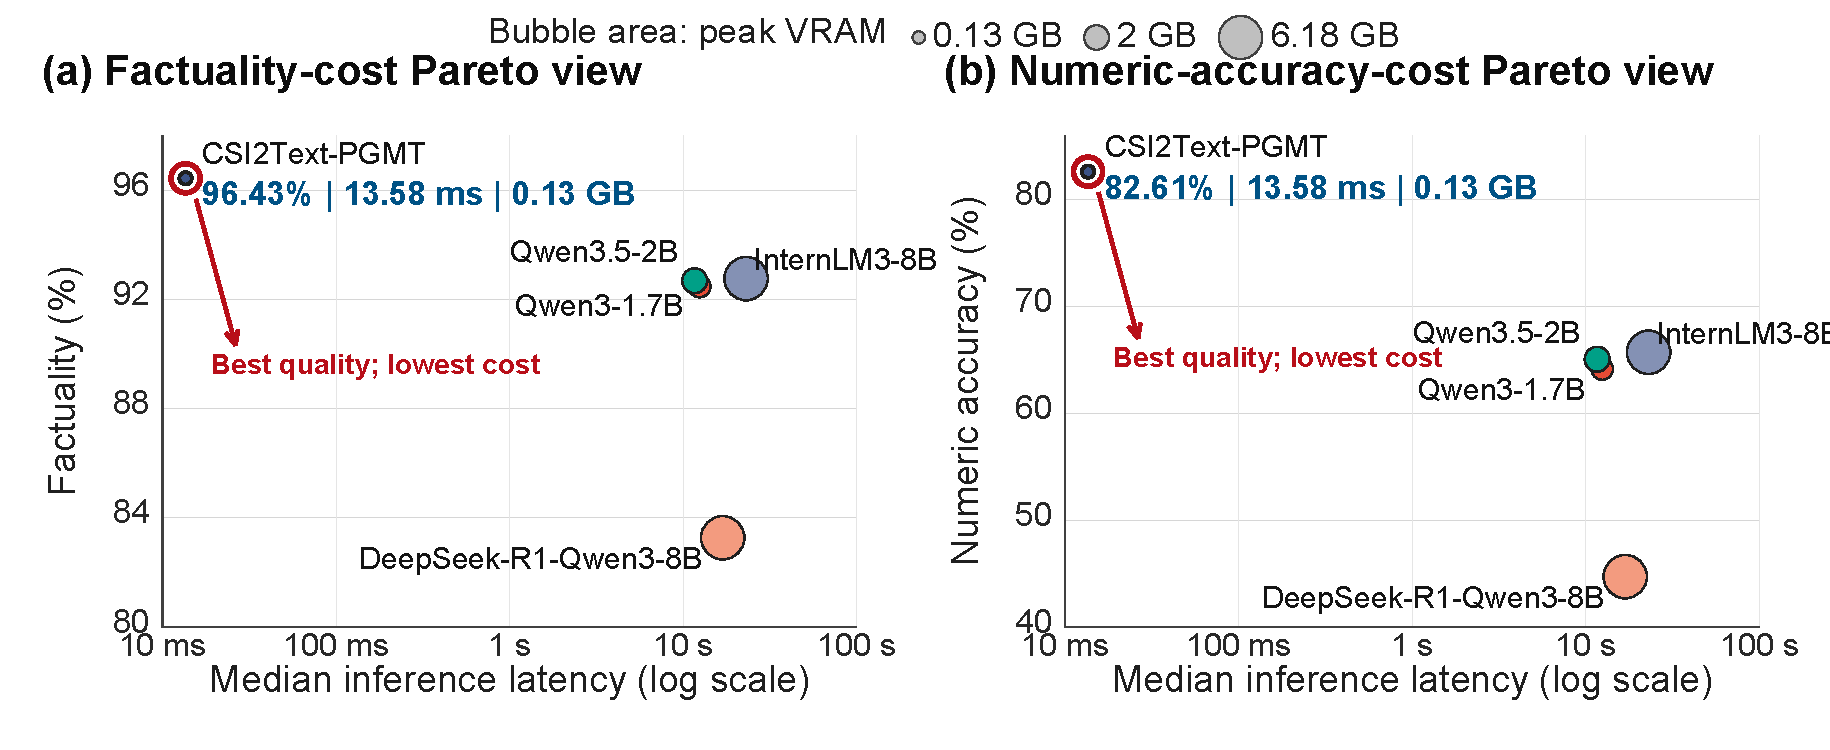
\includegraphics[width=\columnwidth]{quality_cost_pareto_horizontal.pdf}
\end{figure}

Table~\ref{tab:inference-cost-main} and Figure~\ref{fig:quality-cost-pareto} show that direct language
decoding pays a large systems cost in addition to its weaker numerical grounding. The direct decoders
operate on a seconds-per-report scale and allocate far more memory, whereas \model{} remains in the
millisecond regime with a compact physical predictor. Conventional regressors can be slightly faster,
but they do not approach the complete quality profile in Table~\ref{tab:physical-main}. The proposed
pipeline therefore occupies the favorable accuracy--cost corner: it preserves structured factuality
without requiring autoregressive generation for every report.

This distinction matters for radio-network operation, where many candidate links or beams may need
to be evaluated within one scheduling interval. The LLM baselines must keep large backbones resident
and generate output tokens even for a fixed report schema. In contrast, \model{} predicts the
structured record in one feed-forward pass and then uses deterministic verbalization, retaining
physically auditable reports while staying close to the cost profile of compact neural estimators.

\subsection{Generalization}

\subsubsection{Frequency-Configuration Generalization}

\begin{figure}[H]
\centering
\makebox[\columnwidth][c]{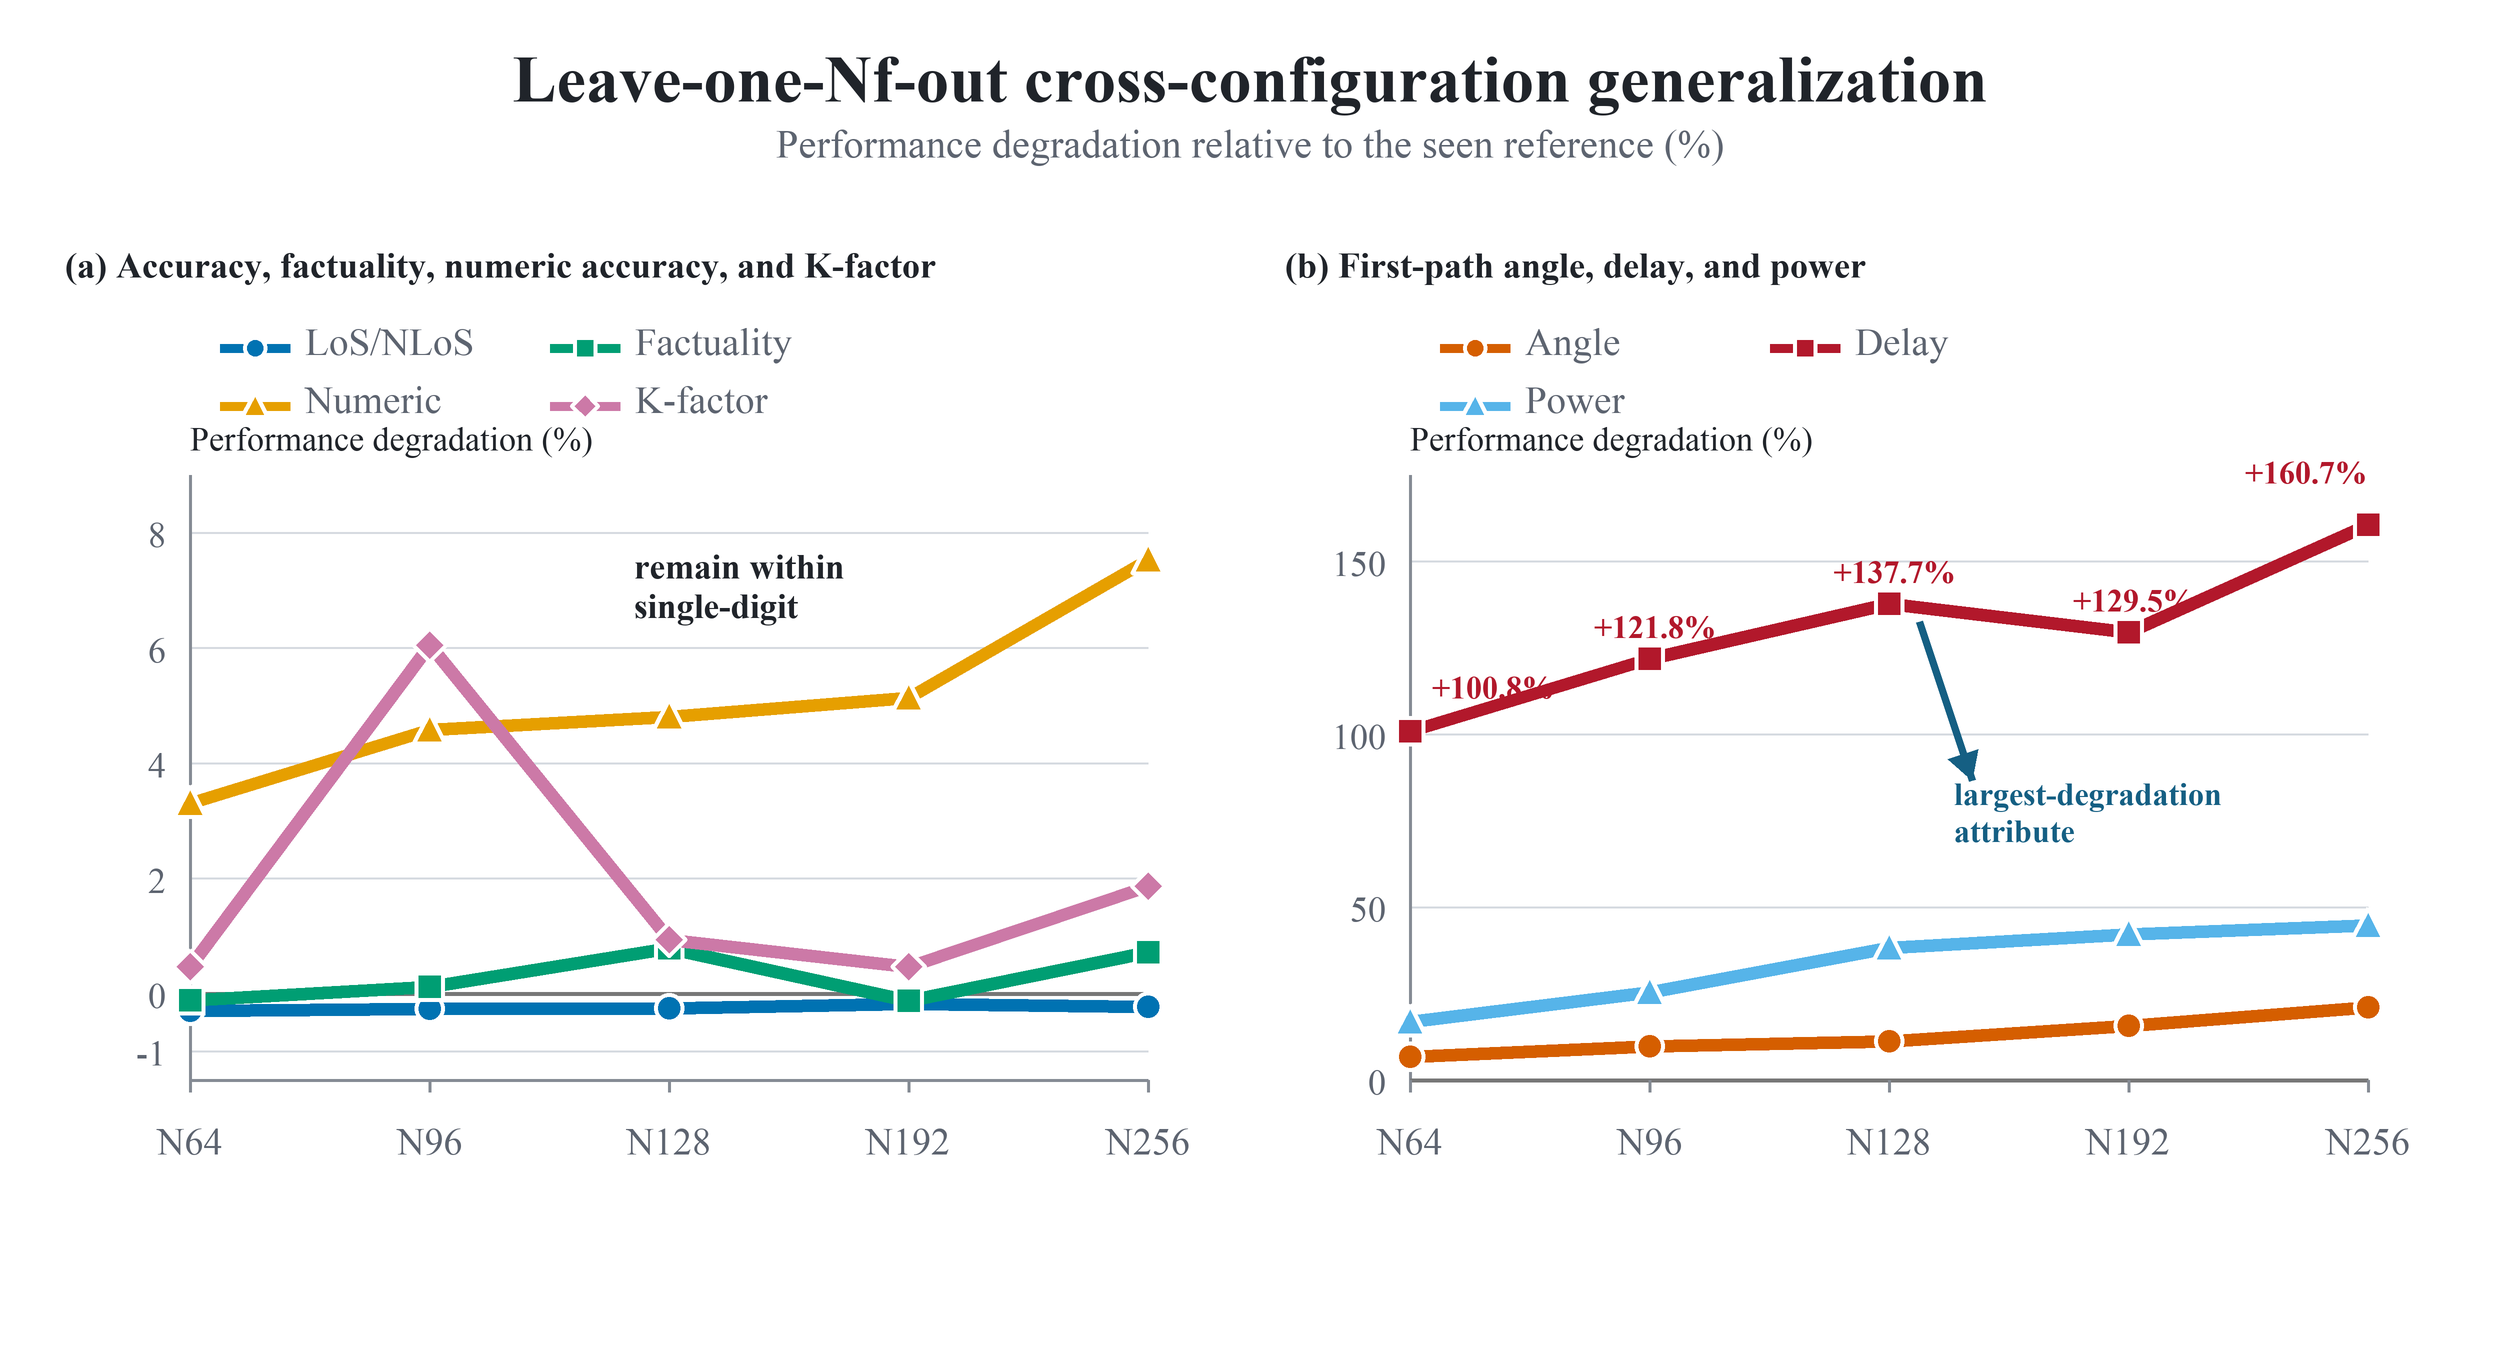
\includegraphics[width=1.12\columnwidth]{figures/leave_one_nf_out_line_panels.png}}
\caption{Leave-one-$N_f$-out generalization. The single-column two-panel line plot reports
performance degradation relative to the seen-$N_f=128$ reference across held-out frequency
samplings. Panel (a) summarizes accuracy, factuality, numeric accuracy, and $K$-factor trends,
whereas panel (b) highlights first-path angle, delay, and power. Positive values indicate worse
held-out performance.}
\label{fig:frequency-generalization}
\end{figure}

For each column of Figure~\ref{fig:frequency-generalization}, the complete model is trained on the
other four values in $\{64,96,128,192,256\}$ and then evaluated on the excluded sampling
configuration. Visibility classification and report factuality remain stable across the held-out
settings, while fine temporal localization is the most sensitive quantity and power or angle exhibit
smaller configuration-dependent changes. The result shows that the configuration-aware
representation transfers semantic channel structure more reliably than it transfers exact delay
resolution. An assisted setting with paired observations from two numerologies is examined separately
as a complementary multi-view extension.

\subsubsection{Cross-Array and Directional Transfer}

We train a mixed-array model with UPA-$8{\times}8$ and ULA-64 observations, then evaluate it on
those seen geometries and on aligned, held-out UPA-$4{\times}4$, UPA-$16{\times}4$, and ULA-32
groups without geometry-specific fine-tuning. A separate pair of experiments reverses the ULA
transfer direction, comparing larger-to-smaller and smaller-to-larger apertures while keeping the
evaluation groups disjoint from training.

\begin{table}[H]
\centering
\caption{Cross-array and directional ULA transfer over three seeds. UPA-$8{\times}8$ and ULA-64 are
seen during mixed-array training. Lower is better for MAE; higher is better for factuality. Panel B
also reports the direction-aware relative change from the seen setting to the unseen setting.}
\label{tab:cross-array}
\scriptsize
\setlength{\tabcolsep}{2.7pt}
\textbf{Panel A: cross-array transfer}\par\vspace{2pt}
\resizebox{\columnwidth}{!}{%
\begin{tabular}{lccccc}
\toprule
\textbf{Array} & \textbf{Status} & \textbf{LoS angle $\downarrow$} &
\textbf{NLoS angle $\downarrow$} & \textbf{First delay $\downarrow$} &
\textbf{Factuality $\uparrow$} \\
\midrule
UPA-$8{\times}8$ & Seen & $6.106\!\pm\!1.966$ & $42.591\!\pm\!0.377$ & $53.854\!\pm\!6.213$ & $94.316\!\pm\!0.096\%$ \\
ULA-64 & Seen & $14.566\!\pm\!2.623$ & $42.710\!\pm\!0.562$ & $47.449\!\pm\!2.121$ & $94.178\!\pm\!0.167\%$ \\
UPA-$4{\times}4$ & Unseen & $10.257\!\pm\!3.013$ & $45.859\!\pm\!0.110$ & $44.082\!\pm\!0.786$ & $93.556\!\pm\!0.092\%$ \\
UPA-$16{\times}4$ & Unseen & $9.446\!\pm\!0.913$ & $43.237\!\pm\!0.114$ & $54.828\!\pm\!5.982$ & $93.639\!\pm\!0.136\%$ \\
ULA-32 & Unseen & $11.345\!\pm\!0.566$ & $42.919\!\pm\!0.400$ & $43.399\!\pm\!1.029$ & $94.449\!\pm\!0.193\%$ \\
\bottomrule
\end{tabular}}
\vspace{3pt}

\textbf{Panel B: directional ULA transfer}\par\vspace{2pt}
\resizebox{\columnwidth}{!}{%
\begin{tabular}{lccccc}
\toprule
\textbf{Direction} & \textbf{Status} & \textbf{LoS angle $\downarrow$} &
\textbf{NLoS angle $\downarrow$} & \textbf{First delay $\downarrow$} &
\textbf{Factuality $\uparrow$} \\
\midrule
$64\rightarrow32$ & Seen 64 & $14.566\!\pm\!2.623$ & $45.613\!\pm\!0.322$ & $47.449\!\pm\!2.121$ & $94.178\!\pm\!0.167\%$ \\
 & Unseen 32 & $11.345\!\pm\!0.566$ & $41.740\!\pm\!0.462$ & $43.399\!\pm\!1.029$ & $94.449\!\pm\!0.193\%$ \\
\rowcolor{gainrow} & \textbf{Unseen vs. seen} & \relgain{22.1\%} & \relgain{8.5\%} & \relgain{8.5\%} & \relgain{0.3\%} \\
\midrule
$32\rightarrow64$ & Seen 32 & $10.730\!\pm\!0.785$ & $42.982\!\pm\!0.112$ & $41.619\!\pm\!0.954$ & $95.092\!\pm\!0.096\%$ \\
 & Unseen 64 & $17.223\!\pm\!3.331$ & $48.592\!\pm\!0.628$ & $49.350\!\pm\!3.524$ & $94.222\!\pm\!0.073\%$ \\
\rowcolor{gainrow} & \textbf{Unseen vs. seen} & \relloss{60.5\%} & \relloss{13.1\%} & \relloss{18.6\%} & \relloss{0.9\%} \\
\bottomrule
\end{tabular}}
\label{tab:directional-ula}
\end{table}

Table~\ref{tab:cross-array} shows that factual report generation remains stable on unseen array shapes
and sizes, while the persistent NLoS-angle error is shared across geometries rather than caused by one
specific array. Directional transfer is asymmetric: learning from the larger aperture transfers cleanly
to the smaller one, whereas extrapolating from a smaller to a larger aperture produces a clearer loss
in angular and temporal precision. The model therefore generalizes across array configurations, but
the training aperture still bounds the reliability of geometric extrapolation.

\subsubsection{Spatial-Block and Map-Disjoint Generalization}

To distinguish local interpolation from environment transfer, we compare a random split with
$32\,\mathrm{m}\times32\,\mathrm{m}$ spatial blocks and complete held-out maps. The audited cohorts
have zero overlap in maps, map-qualified blocks, and user-equipment positions, so the stricter
protocols cannot reuse nearby or identical propagation links from training.

\begin{table}[H]
\centering
\caption{Random, spatial-block, and complete-map-disjoint evaluation. The final column reports the
direction-aware performance difference between map-disjoint evaluation and random splitting.
Higher is better for accuracy; lower is better for MAE. Red denotes an improvement and blue denotes
a degradation. Underlining marks the best result in each row, and boldface highlights the
map-disjoint results.}
\label{tab:split-sensitivity}
\scriptsize
\setlength{\tabcolsep}{2.5pt}
\resizebox{\columnwidth}{!}{%
\begin{tabular}{lcccc}
\toprule
Metric & Random & Spatial block & Map-disjoint & Map-disjoint vs. Random \\
\midrule
Semantic accuracy $\uparrow$ & 0.8750 & \underline{0.8763} & \textbf{0.8618} & \relloss{$1.32$ pp} \\
Semantic macro-F1 $\uparrow$ & 0.5960 & \underline{0.6352} & \textbf{0.4884} & \relloss{$10.76$ pp} \\
First delay (ns) $\downarrow$ & \underline{25.8400} & 31.7410 & \textbf{38.5178} & \relloss{$49.1\%$} \\
LoS delay (ns) $\downarrow$ & \underline{10.2439} & 13.4182 & \textbf{17.5738} & \relloss{$71.6\%$} \\
NLoS delay (ns) $\downarrow$ & \underline{47.4350} & 50.0639 & \textbf{59.4618} & \relloss{$25.4\%$} \\
Delay spread (ns) $\downarrow$ & \underline{14.9583} & 16.5812 & \textbf{18.6648} & \relloss{$24.8\%$} \\
$K$ (dB) $\downarrow$ & \underline{2.4280} & 2.7301 & \textbf{3.2529} & \relloss{$34.0\%$} \\
First power (dB) $\downarrow$ & \underline{4.6009} & 5.2943 & \textbf{6.2998} & \relloss{$36.9\%$} \\
First angle ($^\circ$) $\downarrow$ & 21.8495 & 23.9274 & \textbf{\underline{21.7308}} & \relgain{$0.5\%$} \\
Azimuth spread ($^\circ$) $\downarrow$ & \underline{7.5784} & 10.1609 & \textbf{10.0201} & \relloss{$32.2\%$} \\
Reflection-bin accuracy $\uparrow$ & \underline{0.6599} & 0.5711 & \textbf{0.5498} & \relloss{$11.01$ pp} \\
Path-count MAE $\downarrow$ & 0.1965 & 0.2321 & \textbf{\underline{0.1878}} & \relgain{$4.4\%$} \\
\bottomrule
\end{tabular}}
\end{table}

Table~\ref{tab:split-sensitivity} shows that performance remains usable when evaluation moves from
random interpolation to spatially or map-disjoint transfer. Delay, power, dispersion, and reflection
are more sensitive to unseen environments, whereas first-angle and path-count prediction remain
comparatively stable. The nonuniform change is important: random splitting is optimistic for selected
physical quantities, but the retained semantic and structural performance demonstrates meaningful
generalization beyond memorized locations.

\subsection{Robustness}

We evaluate robustness by perturbing the observed complex CSI with additive white Gaussian noise
(AWGN) during both training and testing. For each sample, noise is applied only to the valid,
non-padding index set \(\Omega\). Given a target signal-to-noise ratio \(\gamma\) in decibels, the
corrupted CSI is
\begin{equation}
\begin{aligned}
\widetilde{\mathbf H}&=\mathbf H+\mathbf N, &
P_H&=\frac{1}{|\Omega|}\sum_{u\in\Omega}|H_u|^2,\\
P_N&=P_H10^{-\gamma/10}, &
\Re(N_u),\Im(N_u)&\sim\mathcal N(0,P_N/2),
\end{aligned}
\label{eq:complex-awgn}
\end{equation}
where \(\mathbb E|N_u|^2=P_N\). During noise-augmented training, each batch is independently
selected for corruption with \(z_b\sim\operatorname{Bernoulli}(0.8)\), and its SNR is sampled as
\(\gamma_b\sim\mathcal U(10,30)\) dB. After warm-up, the batch objective is
\begin{equation}
\begin{aligned}
\mathcal L_b={}&\mathcal L_{\mathrm{clean}}+0.2\mathcal L_{K,\mathrm{clean}}\\
&+z_b\bigl[0.5\mathcal L_{\mathrm{noisy}}+0.1\mathcal L_{\tau,\mathrm{cons}}\\
&\hspace{18mm}+0.1\mathcal L_{K,\mathrm{cons}}
+0.1\mathcal L_{K,\mathrm{noisy}}\bigr],
\end{aligned}
\label{eq:noise-training}
\end{equation}
where the supervised terms are masked Smooth-L1 losses and the consistency terms compare noisy
predictions with stop-gradient clean predictions in normalized physical-target space. Testing uses
freshly sampled noise at \(\gamma\in\{30,20,10,0\}\) dB, together with an uncorrupted reference set,
so the evaluation measures generalization to unseen noise realizations rather than reuse of the
training perturbations.

For each trained model seed \(s\), every metric is first averaged over three independent test-noise
realizations \(r\), and the final mean and sample standard deviation are then computed over three
model seeds:
\begin{equation}
\begin{aligned}
\bar M_s&=\frac{1}{3}\sum_{r=1}^{3}M_{s,r},&
\mu_M&=\frac{1}{3}\sum_{s=1}^{3}\bar M_s,\\
\sigma_M&=\sqrt{\frac{1}{2}\sum_{s=1}^{3}(\bar M_s-\mu_M)^2}.
\end{aligned}
\label{eq:awgn-seed-statistics}
\end{equation}
For a lower-is-better metric, the relative degradation at SNR \(\gamma\) is
\begin{equation}
D_M(\gamma)=
\frac{M(\gamma)-M(\mathrm{clean})}{M(\mathrm{clean})}\times100\%.
\label{eq:relative-noise-degradation}
\end{equation}

\begin{table}[H]
\centering
\caption{Three-seed test-time complex-AWGN robustness. Lower is better for MAE; higher is better
for numerical tolerance accuracy.}
\label{tab:awgn}
\scriptsize
\setlength{\tabcolsep}{4pt}
\resizebox{\columnwidth}{!}{%
\begin{tabular}{lccccc}
\toprule
Metric & Clean & 30 dB & 20 dB & 10 dB & 0 dB \\
\midrule
First delay (ns) $\downarrow$ & $25.97\!\pm\!0.34$ & $72.70\!\pm\!0.40$ & $86.11\!\pm\!0.96$ & $100.23\!\pm\!1.73$ & $209.29\!\pm\!12.31$ \\
LoS delay (ns) $\downarrow$ & $8.72\!\pm\!0.49$ & $20.30\!\pm\!2.71$ & $25.00\!\pm\!2.43$ & $34.10\!\pm\!1.32$ & $231.85\!\pm\!28.52$ \\
NLoS delay (ns) $\downarrow$ & $43.22\!\pm\!0.27$ & $125.10\!\pm\!3.05$ & $147.22\!\pm\!2.52$ & $166.36\!\pm\!4.31$ & $186.73\!\pm\!6.54$ \\
First angle ($^\circ$) $\downarrow$ & $18.84\!\pm\!0.40$ & $23.10\!\pm\!0.84$ & $24.29\!\pm\!0.71$ & $25.12\!\pm\!0.79$ & $32.30\!\pm\!1.92$ \\
First power (dB) $\downarrow$ & $5.12\!\pm\!0.35$ & $4.88\!\pm\!0.37$ & $4.79\!\pm\!0.37$ & $5.38\!\pm\!0.58$ & $17.69\!\pm\!0.08$ \\
$K$ (dB) $\downarrow$ & $2.084\!\pm\!0.124$ & $2.142\!\pm\!0.125$ & $2.612\!\pm\!0.118$ & $5.978\!\pm\!0.582$ & $19.855\!\pm\!0.659$ \\
Reflection-path MAE $\downarrow$ & $1.018\!\pm\!0.014$ & $1.180\!\pm\!0.006$ & $1.232\!\pm\!0.011$ & $1.338\!\pm\!0.009$ & $2.384\!\pm\!0.178$ \\
Numeric accuracy (\%) $\uparrow$ & $74.05\!\pm\!0.57$ & $69.27\!\pm\!0.65$ & $64.91\!\pm\!0.82$ & $56.22\!\pm\!1.01$ & $33.93\!\pm\!2.18$ \\
\bottomrule
\end{tabular}}
\end{table}

\begin{figure}[H]
\centering
\caption{Test-time complex-AWGN robustness. Panel (a) reports the absolute MAE of first-path,
LoS, and NLoS delay; panel (b) reports first-angle, first-power, and \(K\)-factor MAE normalized by
their clean-condition values, focusing the comparison on physical prediction robustness.}
\label{fig:awgn-robustness}
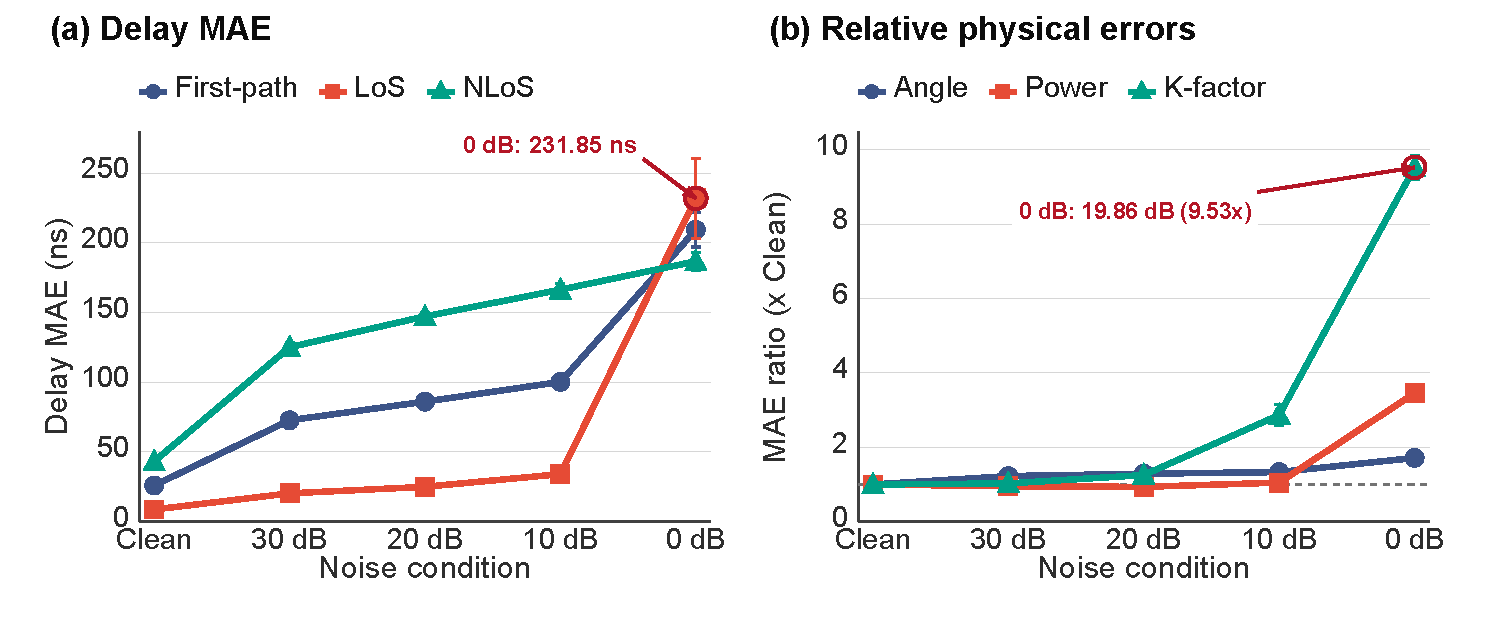
\includegraphics[width=\columnwidth]{figures/awgn_robustness_ab.pdf}
\end{figure}

Table~\ref{tab:awgn} and Figure~\ref{fig:awgn-robustness} show that degradation is monotonic overall
but strongly attribute dependent. Delay is affected first because it is encoded by phase variation
across frequency. The NLoS delay curve rises much faster than the LoS curve at moderate SNR, which
is consistent with the difficulty of locating the earliest indirect component among several
overlapping reflections. First-angle error grows more gradually, indicating that coarse spatial
structure survives moderate corruption better than fine temporal localization.

Power and \(K\)-factor remain close to their clean baselines at moderate noise levels but deteriorate
sharply when the SNR approaches 0 dB. The small fluctuation in power error at 20--30 dB lies within
the reported seed variation and should not be interpreted as an improvement. Reflection-path error
also increases steadily, while numerical tolerance accuracy in Table~\ref{tab:awgn} decreases as more
fields leave their accepted ranges. Overall, noise augmentation preserves useful physical predictions
under moderate corruption, but it cannot recover channel evidence destroyed by severe noise. This
attribute-specific behavior supports confidence-aware use: coarse state may remain usable even when
a precise delay or power value should be withheld.

\subsection{Ablation}

\subsubsection{Language-Alignment Ablation}

Language alignment provides semantic organization for the shared CSI representation before the
physical heads produce their structured outputs. The CSI--text objective associates each sample with
its complete channel description, whereas text--prototype alignment pulls semantically similar
samples toward coarse propagation prototypes such as LoS/NLoS regime and path-richness categories.
These language branches are used as training-time regularizers and are removed at inference, so their
effect can be isolated without changing deployment cost. Intuitively, the alignment losses do not ask
the text branch to generate the final answer; instead, they shape the CSI embedding so that samples
with similar propagation semantics occupy nearby regions before the numerical heads are applied. This
is useful because several targets are not independent: visibility, path count, reflection strength,
and delay spread jointly describe the same propagation regime. A representation that already encodes
this coarse regime gives the downstream heads a narrower and more physically plausible search space.

We construct matched variants that remove CSI--text alignment, text--prototype alignment, or both
(the physics-only setting), while keeping the physical heads, target supervision, correction rules,
data split, and verbalizer fixed. Table~\ref{tab:language-ablation} therefore measures the contribution
of semantic alignment rather than additional inference-time capacity.

\begin{table}[H]
\centering
\caption{Matched language-alignment ablations over three seeds. Higher is better for classification
and bin accuracy; lower is better for MAE. The final row in each block compares the full model with
the best ablated variant for each metric (red: improvement; blue: degradation). Underlining marks
the best result across all variants, including the full model.}
\label{tab:language-ablation}
\scriptsize
\setlength{\tabcolsep}{2.7pt}
\resizebox{\columnwidth}{!}{%
\begin{tabular}{lcccc}
\toprule
\textbf{Variant} & \textbf{LoS/NLoS acc. $\uparrow$} & \textbf{Delay (ns) $\downarrow$} &
\textbf{Refl. MAE $\downarrow$} & \textbf{Refl. acc. $\uparrow$} \\
\midrule
\rowcolor{modelblue}\textbf{Full alignment} & $\best{\boldsymbol{0.99572\!\pm\!0.00314}}$ & $\best{\boldsymbol{25.9495\!\pm\!1.2610}}$ & $\best{\boldsymbol{1.0644\!\pm\!0.0164}}$ & $\best{\boldsymbol{0.6866\!\pm\!0.0053}}$ \\
\textbf{No CSI--text} & $0.99297\!\pm\!0.00080$ & $27.3459\!\pm\!0.9163$ & $1.0776\!\pm\!0.0069$ & $0.6579\!\pm\!0.0022$ \\
\textbf{No text--prototype} & $0.99330\!\pm\!0.00006$ & $28.3746\!\pm\!0.2799$ & $1.0925\!\pm\!0.0100$ & $0.6521\!\pm\!0.0092$ \\
\textbf{Physics only} & $0.98313\!\pm\!0.00071$ & $27.6446\!\pm\!0.8540$ & $1.1170\!\pm\!0.0135$ & $0.6280\!\pm\!0.0062$ \\
\midrule
\rowcolor{gainrow}\textbf{Rel. change vs. best ablation} & \relgain{$0.2\%$} & \relgain{$5.1\%$} & \relgain{$1.2\%$} & \relgain{$4.4\%$} \\
\bottomrule
\end{tabular}}
\vspace{2pt}

\resizebox{\columnwidth}{!}{%
\begin{tabular}{lccc}
\toprule
\textbf{Variant} & \textbf{Path MAE $\downarrow$} &
\textbf{NLoS power $\downarrow$} & \textbf{NLoS angle $\downarrow$} \\
\midrule
\rowcolor{modelblue}\textbf{Full alignment} & $\best{\boldsymbol{0.2106\!\pm\!0.0102}}$ & $\best{\boldsymbol{7.3023\!\pm\!0.2223}}$ & $\best{\boldsymbol{38.3226\!\pm\!0.7280}}$ \\
\textbf{No CSI--text} & $0.2130\!\pm\!0.0144$ & $7.4089\!\pm\!0.1944$ & $39.6833\!\pm\!0.7642$ \\
\textbf{No text--prototype} & $0.2144\!\pm\!0.0559$ & $7.3636\!\pm\!0.0424$ & $39.6135\!\pm\!1.2067$ \\
\textbf{Physics only} & $0.3736\!\pm\!0.0551$ & $8.3348\!\pm\!0.5728$ & $39.2445\!\pm\!1.3988$ \\
\midrule
\rowcolor{gainrow}\textbf{Rel. change vs. best ablation} & \relgain{$1.1\%$} & \relgain{$0.8\%$} & \relgain{$2.3\%$} \\
\bottomrule
\end{tabular}}
\end{table}

The aligned model is strongest on categorical and structure-related labels, especially LoS/NLoS
discrimination, path count, reflection-path MAE, and reflection-bin accuracy, while also giving
smaller but consistent gains for delay and ambiguous NLoS angle or power. This suggests that
language prototypes first narrow the coarse propagation regime and path-structure category, after
which CSI--text alignment refines the representation with sample-specific attributes. The two
alignment terms therefore play complementary roles: prototypes supply global semantic anchors, while
instance descriptions preserve the detailed sample-level relations needed for continuous regression.
The largest gains on reflection and path-count metrics are consistent with this interpretation,
because those targets depend on recognizing the overall multipath structure rather than reading a
single isolated scalar from the CSI. Because every variant still receives direct physical labels, the
comparison supports language alignment as a structural regularizer for physical supervision rather
than a replacement for it.

\subsubsection{Physical Prediction-Head Ablations}

The physical estimator is deliberately factorized into a shared configuration encoder and shared
physics token, followed by multiple target-specific encoders and prediction heads for delay, angle,
power, and path structure. This multi-encoder, multi-head design allows coupled evidence to be reused
while retaining the inductive bias appropriate to each physical quantity. We remove one component or
auxiliary constraint at a time and evaluate only the labels most directly related to that intervention.
Table~\ref{tab:physical-head-ablation} combines the angle, structural, and temporal/power studies.

\begin{table}[H]
\centering
\caption{Target-specific physical prediction-head ablations over three seeds. Each panel retains only
labels related to the removed component; lower is better unless indicated otherwise. The final row
compares the full model with the best ablated variant for each metric (red: improvement; blue:
degradation). Underlining marks the best result across all variants, including the full model.}
\label{tab:physical-head-ablation}
\label{tab:angle-ablation}
\label{tab:reflection-ablation}
\label{tab:architecture-ablation}
\scriptsize
\setlength{\tabcolsep}{3.0pt}
\renewcommand{\arraystretch}{0.96}
\textbf{Panel A: angle encoders}\par\vspace{1pt}
\resizebox{\linewidth}{!}{%
\begin{tabular}{lccc}
\toprule
\textbf{Variant} & \textbf{LoS angle $\downarrow$} & \textbf{First-angle LoS $\downarrow$} &
\textbf{First-angle NLoS $\downarrow$} \\
\midrule
\rowcolor{modelblue}\textbf{Full} & $\best{\boldsymbol{1.3564\!\pm\!0.1419}}$ & $\best{\boldsymbol{1.6798\!\pm\!0.0434}}$ & $\best{\boldsymbol{35.2717\!\pm\!0.7477}}$ \\
\textbf{No LoS-angle encoder} & $16.3092\!\pm\!0.2847$ & $5.9300\!\pm\!0.0964$ & $39.8998\!\pm\!1.0083$ \\
\textbf{No first-angle encoder} & $1.8599\!\pm\!0.2485$ & $2.3328\!\pm\!0.0427$ & $43.5819\!\pm\!0.0074$ \\
\midrule
\rowcolor{gainrow}\textbf{Rel. change vs. best ablation} & \relgain{$27.1\%$} & \relgain{$28.0\%$} & \relgain{$11.6\%$} \\
\bottomrule
\end{tabular}}

\vspace{2pt}
\textbf{Panel B: structural objectives}\par\vspace{1pt}
\resizebox{\linewidth}{!}{%
\begin{tabular}{lccc}
\toprule
\textbf{Variant} & \textbf{Reflection MAE $\downarrow$} &
\textbf{Reflection acc. $\uparrow$} & \textbf{Path-count MAE $\downarrow$} \\
\midrule
\rowcolor{modelblue}\textbf{Full} & $\best{\boldsymbol{0.9833\!\pm\!0.0054}}$ & $\best{\boldsymbol{0.7061\!\pm\!0.0039}}$ & $\best{\boldsymbol{0.1539\!\pm\!0.0079}}$ \\
\textbf{No reflection auxiliary loss} & $8.2848\!\pm\!0.0138$ & $0.1741\!\pm\!0.0028$ & $0.1972\!\pm\!0.0185$ \\
\textbf{No LoS consistency} & $1.0765\!\pm\!0.1479$ & $0.6548\!\pm\!0.4725$ & $0.2228\!\pm\!0.0088$ \\
\midrule
\rowcolor{gainrow}\textbf{Rel. change vs. best ablation} & \relgain{$8.7\%$} & \relgain{$7.8\%$} & \relgain{$22.0\%$} \\
\bottomrule
\end{tabular}}

\vspace{2pt}
\textbf{Panel C: shared, delay, and power components}\par\vspace{1pt}
\resizebox{\linewidth}{!}{%
\begin{tabular}{lccc}
\toprule
\textbf{Variant} & \textbf{Delay $\downarrow$} & \textbf{LoS delay $\downarrow$} &
\textbf{NLoS delay $\downarrow$} \\
\midrule
\rowcolor{modelblue}\textbf{Full} & $\best{\boldsymbol{21.9112\!\pm\!0.3031}}$ & $\best{\boldsymbol{8.1737\!\pm\!0.1556}}$ & $\best{\boldsymbol{35.8198\!\pm\!0.5986}}$ \\
\textbf{No shared token} & $22.6218\!\pm\!0.7071$ & $9.8156\!\pm\!0.6196$ & $36.6103\!\pm\!0.8507$ \\
\textbf{No delay encoder} & $69.0200\!\pm\!1.4595$ & $15.9316\!\pm\!0.8742$ & $130.8691\!\pm\!2.2043$ \\
\textbf{No power} & $29.3139\!\pm\!0.7274$ & $11.0429\!\pm\!1.0211$ & $47.7919\!\pm\!0.2816$ \\
\midrule
\rowcolor{gainrow}\textbf{Rel. change vs. best ablation} & \relgain{$3.1\%$} & \relgain{$16.7\%$} & \relgain{$2.2\%$} \\
\bottomrule
\end{tabular}}

\vspace{2pt}
\textbf{Panel D: spread, $K$, and power components}\par\vspace{1pt}
\resizebox{\linewidth}{!}{%
\begin{tabular}{lccc}
\toprule
\textbf{Variant} & \textbf{Spread $\downarrow$} & \textbf{$K$ $\downarrow$} &
\textbf{Power $\downarrow$} \\
\midrule
\rowcolor{modelblue}\textbf{Full} & $\best{\boldsymbol{11.1419\!\pm\!0.1068}}$ & $\boldsymbol{1.8829\!\pm\!0.2633}$ & $\boldsymbol{4.9575\!\pm\!0.2686}$ \\
\textbf{No shared token} & $11.1766\!\pm\!0.0753$ & $\best{1.7426\!\pm\!0.0419}$ & $\best{4.5792\!\pm\!0.0306}$ \\
\textbf{No delay encoder} & $29.6388\!\pm\!0.8355$ & $2.5399\!\pm\!0.1149$ & $5.7443\!\pm\!0.2547$ \\
\textbf{No power} & $14.1139\!\pm\!0.3321$ & $2.2289\!\pm\!0.1659$ & $4.8605\!\pm\!0.7743$ \\
\midrule
\rowcolor{gainrow}\textbf{Rel. change vs. best ablation} & \relgain{$0.3\%$} & \relloss{$8.1\%$} & \relloss{$8.3\%$} \\
\bottomrule
\end{tabular}}
\end{table}

The effects are localized to the labels matched to each removed component. Without the LoS-angle
encoder, LoS-angle estimation deteriorates sharply; without the first-angle encoder, the largest
penalty appears on NLoS first-angle prediction. Removing the reflection auxiliary objective produces
the most pronounced structural failure, simultaneously worsening reflection regression,
reflection-bin classification, and path-count estimation. The LoS-consistency term also supports
these coupled structural labels.

The delay encoder is indispensable for temporal estimation: removing it degrades first-path delay,
especially in NLoS, and also harms delay spread. Removing the raw-power branch affects not only
absolute power evidence but also delay and \(K\)-factor, confirming that scale information is shared
across the structured record. The shared token shows a smaller, mixed per-label effect, as expected
under multitask competition, but generally improves the coherence of the coupled outputs.

Taken together, the panels show why neither a single undifferentiated head nor fully independent
regressors are sufficient. Specialized heads provide target-matched representations, while shared
encoding transfers propagation-regime, path-prominence, and absolute-scale evidence across related
quantities. An occasional isolated metric improvement after removing a component does not overturn
the joint result; it reflects reduced multitask competition at the cost of other dependent labels.
The full multi-encoder, multi-head architecture is therefore necessary for a consistently accurate
and physically coherent channel record.
\subsection{Failure Modes and Error Analysis}

\setcounter{figure}{5}
\begin{figure}[H]
\centering
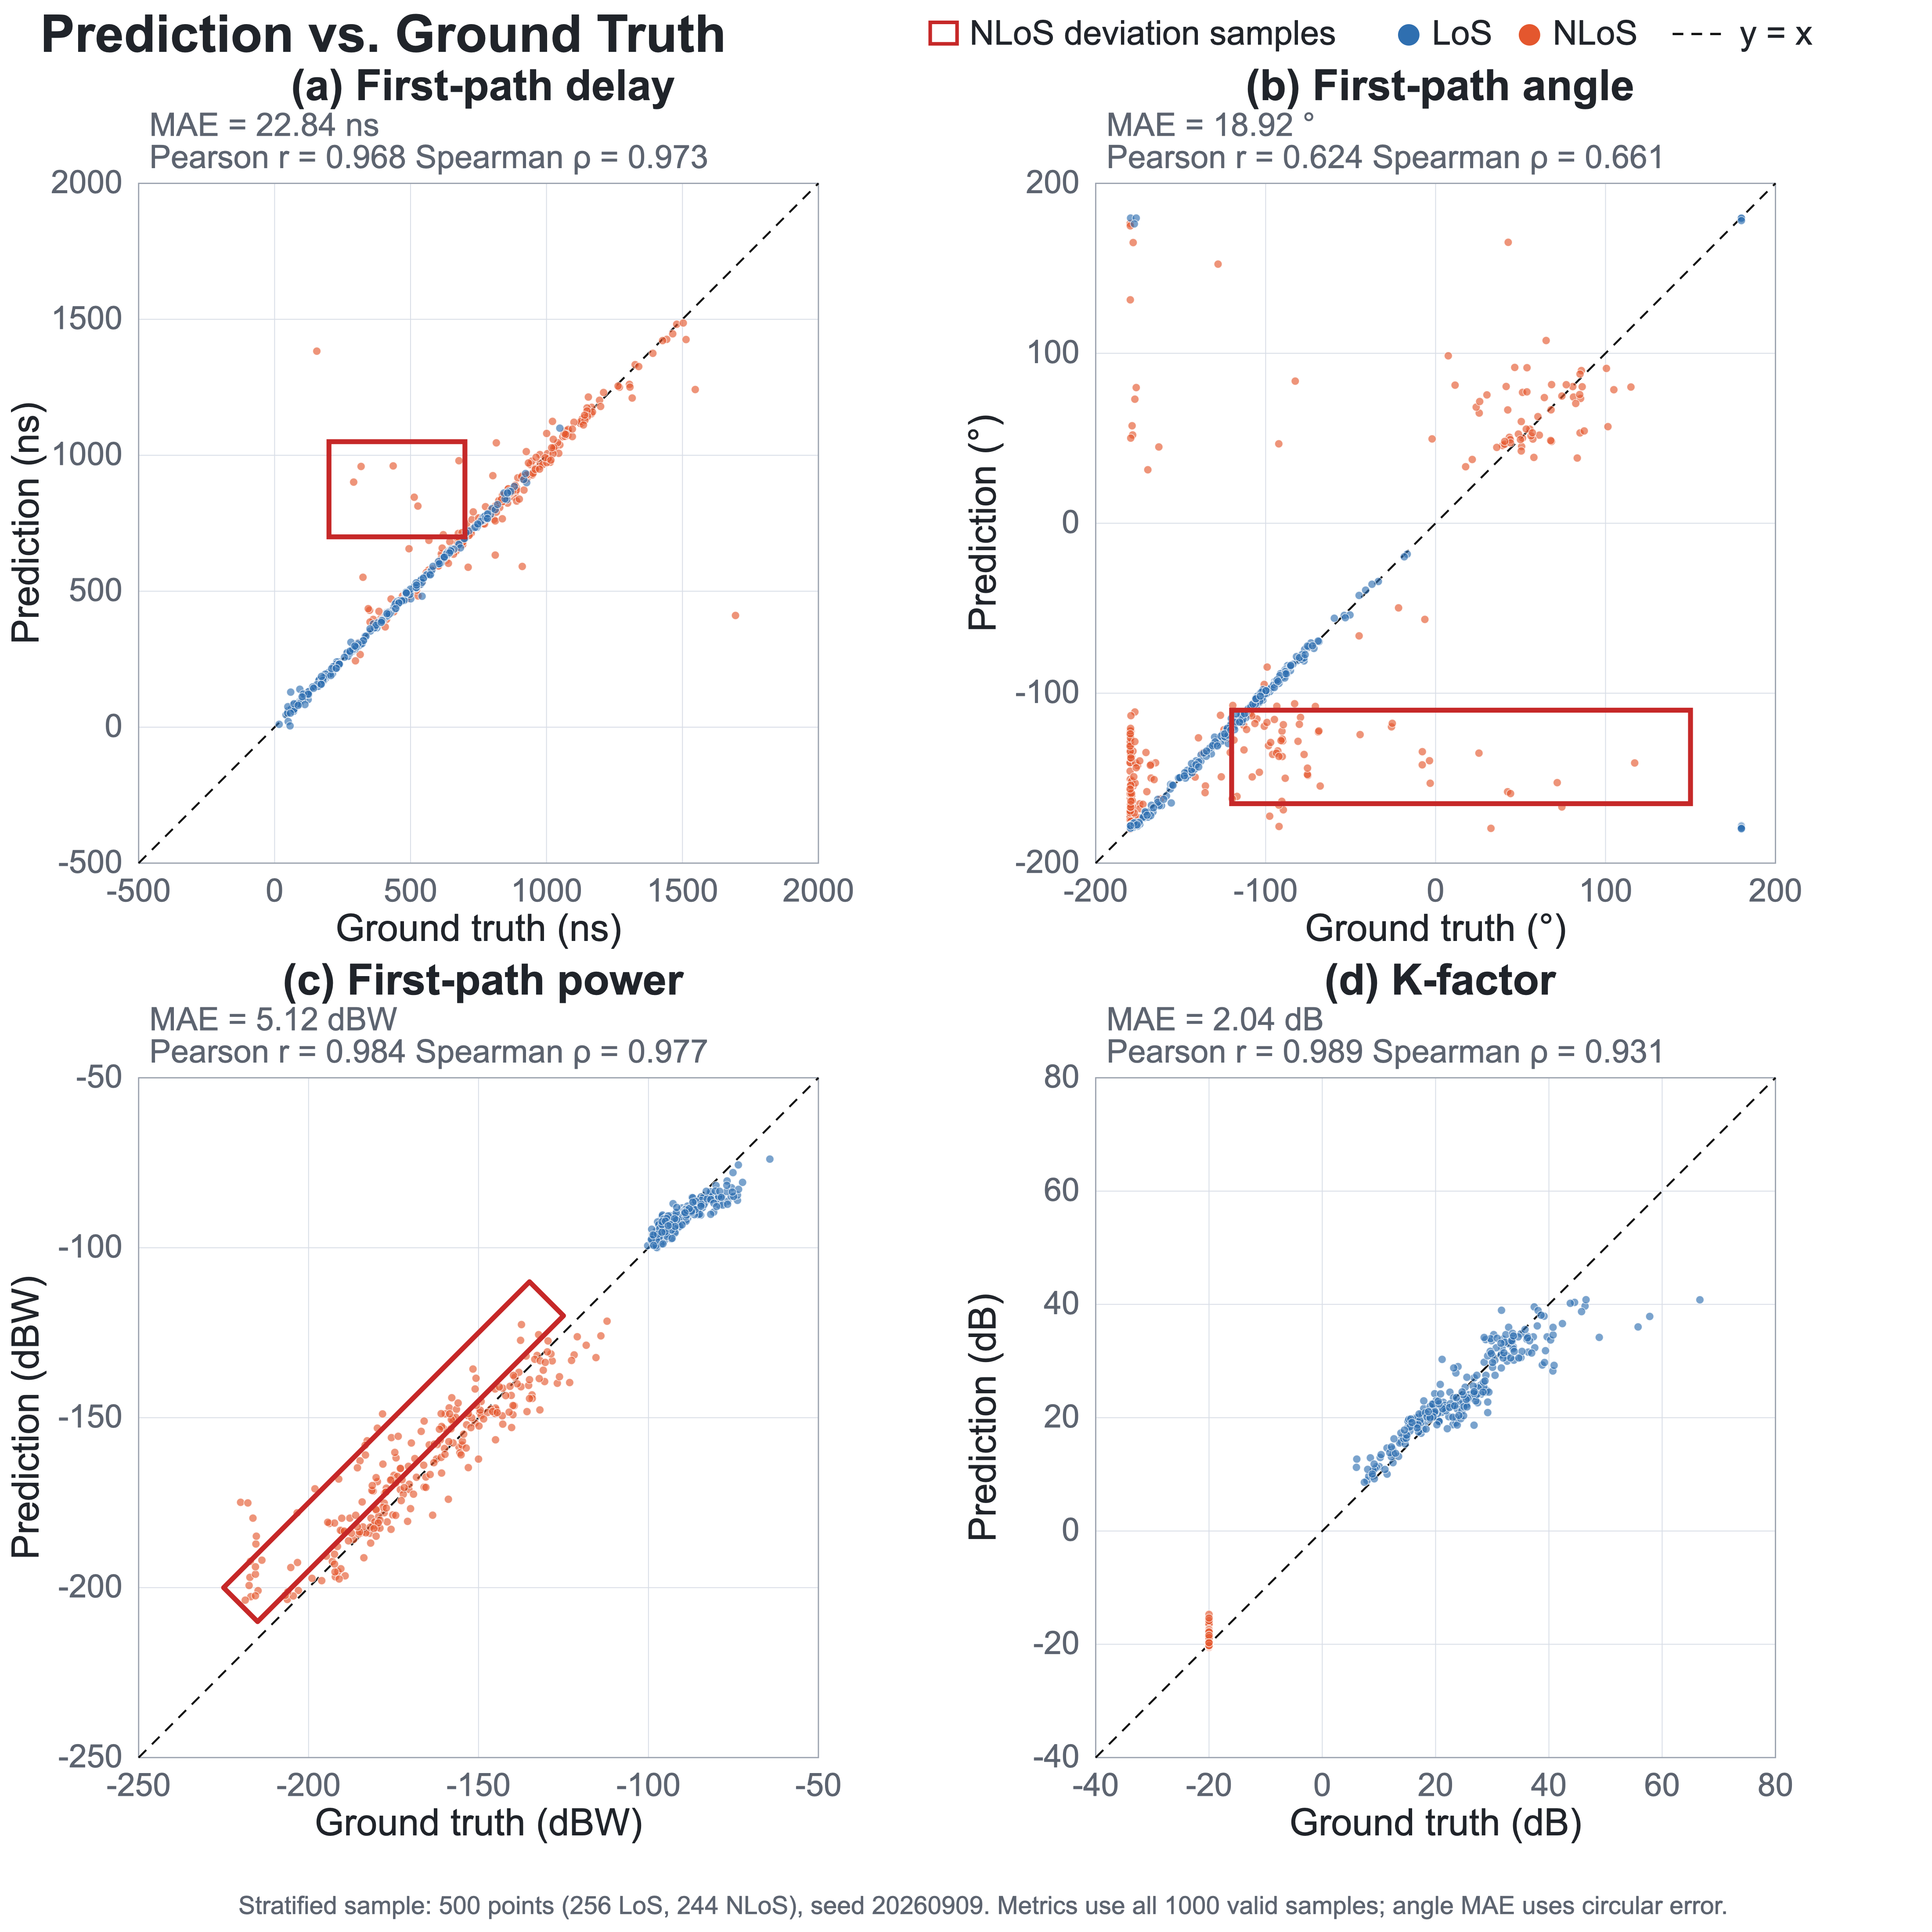
\includegraphics[width=\columnwidth]{figures/prediction_vs_ground_truth_compact.png}
\caption{Per-sample predictions against ground truth for four principal continuous attributes. The
display contains a LoS/NLoS-stratified sample of 500 points, while the reported statistics use all
1,000 valid examples. Delay, power, and \(K\)-factor closely follow the identity line; first-angle
predictions show substantially larger NLoS dispersion. Red boxes identify representative regions
containing deviated NLoS samples. Angle error is circular.}
\label{fig:prediction-ground-truth}
\end{figure}

Figure~\ref{fig:prediction-ground-truth} first reveals that the dominant failures are concentrated in
NLoS samples rather than distributed uniformly across the test set. Delay, power, and \(K\)-factor
remain strongly ordered overall: their Pearson correlations are 0.968, 0.984, and 0.989, respectively,
and most LoS points lie close to the identity line. The largest delay outliers, the compressed
high-\(K\) region, and the broader power deviations are nevertheless predominantly NLoS cases.
First-angle prediction is the clearest failure mode. Its Pearson and Spearman correlations fall to
0.624 and 0.661, and the NLoS samples form broad off-diagonal groups even after circular angle
error is used. The figure therefore indicates that the remaining error is principally a
propagation-regime and observability problem, not a uniform calibration failure of the model.

\setcounter{figure}{4}
\noindent
\begin{minipage}[t]{0.50\columnwidth}
\vspace{0pt}
Figure~\ref{fig:los-nlos} quantifies the regime gap exposed by
Figure~\ref{fig:prediction-ground-truth}. Relative to LoS, NLoS increases first-delay, first-angle,
and first-power MAE by \(4.38\times\), \(21.0\times\), and \(2.34\times\), respectively.
\end{minipage}\hfill
\begin{minipage}[t]{0.47\columnwidth}
\vspace{0pt}
\centering
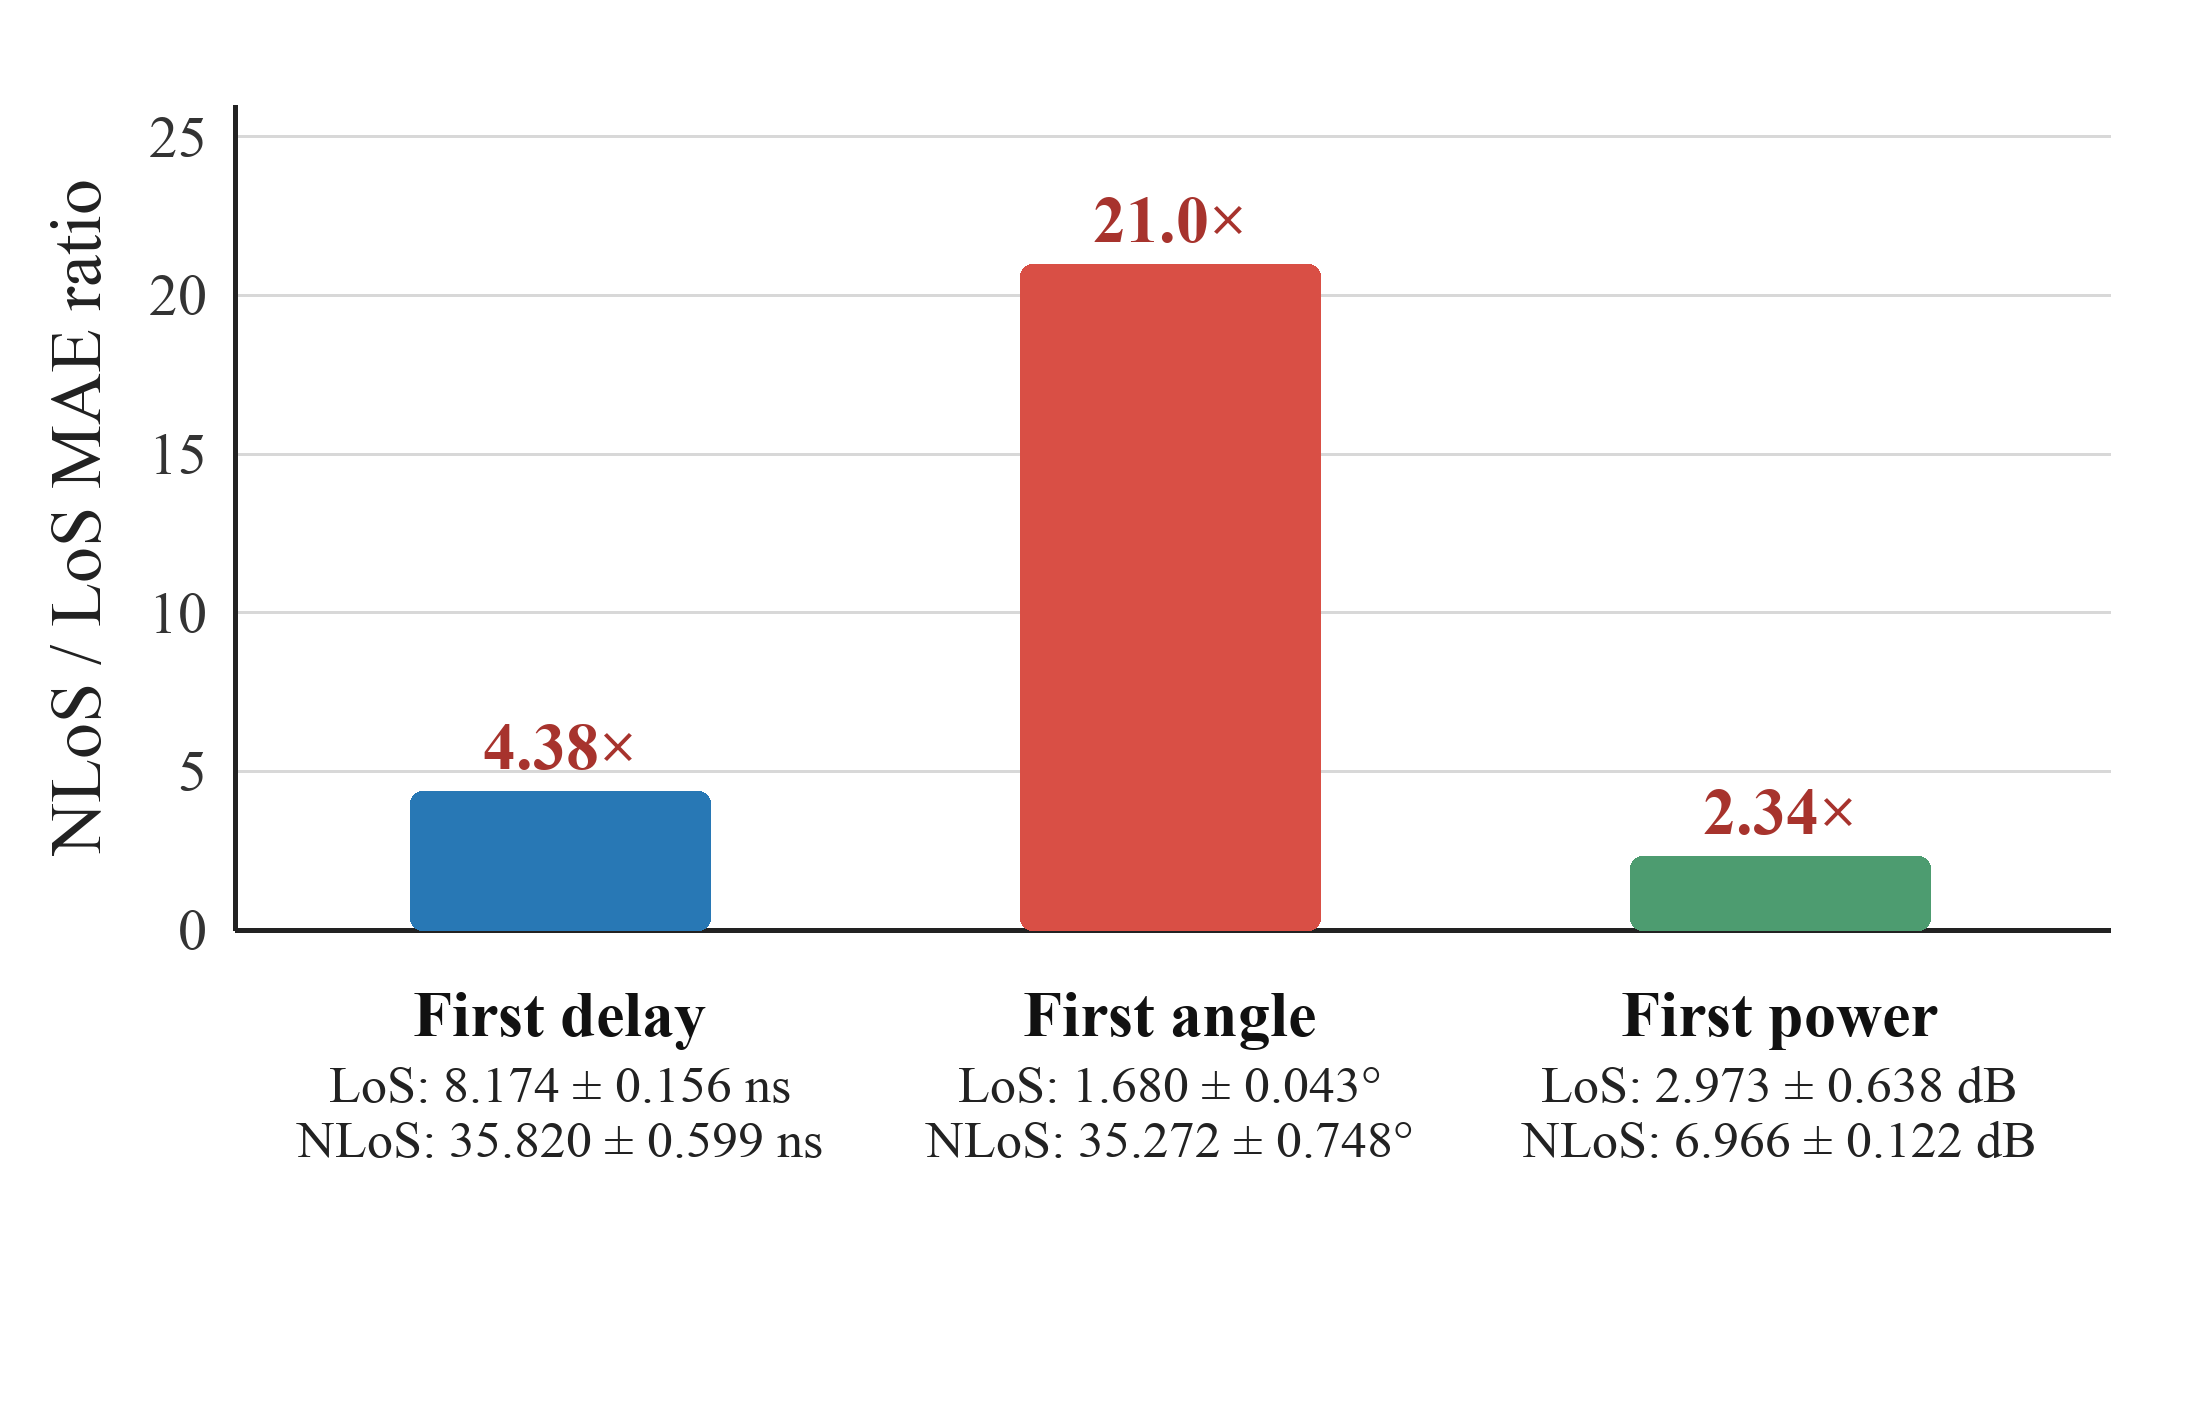
\includegraphics[width=\linewidth]{figures/los_nlos_ratio.png}
\captionsetup{font=scriptsize,skip=1pt}
\captionof{figure}{Propagation-regime error gap. Bars report the NLoS-to-LoS MAE ratio; labels retain the
underlying LoS and NLoS mean \(\pm\) standard deviation.}
\label{fig:los-nlos}
\end{minipage}
\setcounter{figure}{6}

Consequently, one aggregate MAE can conceal the fact that the balanced test set combines a
comparatively easy direct-path regime with a much harder indirect-path regime. The particularly
large angle ratio also explains why satisfactory average performance does not imply that every
reported NLoS field is equally reliable.

The gap mainly follows from observability. In LoS, the earliest component is tied to a direct path
with stable phase, spatial signature, and power ordering. In NLoS, the first retained component is a
reflection, and several reflected paths can have similar delays and powers, so small representation
errors may change which path is treated as dominant. The problem is amplified because the input keeps
only one receive element: receiver-side angle must be inferred indirectly from transmit-side
beam--frequency structure and statistical geometry correlations rather than resolved by a receive
array. Richer receive-side views, paired numerologies, geometry-aware priors, or NLoS-focused
training could reduce this ambiguity; when they are unavailable, high-risk NLoS cases should be
deferred or reviewed rather than forced into an automatic report, motivating the selective-prediction
mechanism below.

\subsection{Reliability-Aware Selective Prediction}

Reliable channel reporting requires more than a low average error: the system must also recognize
when an individual prediction should not be trusted. This is especially important for the NLoS tail
identified in Section~IV-E, where a small number of large delay or angle errors can affect downstream
beam management, localization, and channel interpretation even when the aggregate metric remains
acceptable. Reliability-aware selective prediction converts this requirement into an explicit
coverage--risk trade-off. Low-uncertainty reports are emitted automatically, while uncertain samples
are deferred for an additional observation, an alternative frequency configuration, or human review.
In this setting, deferral is not treated as a failure of the predictor. It is an operational decision:
the system should provide a report when the physical evidence is stable, and it should withhold or
verify a report when the model ensemble disagrees about the underlying channel attributes. This is
especially relevant for autonomous wireless controllers, where a single erroneous NLoS angle or delay
estimate can lead to a wrong beam, a poor localization update, or an overconfident channel summary.

We estimate uncertainty from disagreement among \(S=3\) independently trained models. For sample
\(i\), the ensemble prediction and its sample standard deviation are
\begin{equation}
\bar y_i=\frac{1}{S}\sum_{s=1}^{S}\hat y_i^{(s)},\qquad
u_i=\sqrt{\frac{1}{S-1}\sum_{s=1}^{S}
\left(\hat y_i^{(s)}-\bar y_i\right)^2},
\label{eq:ensemble-uncertainty}
\end{equation}
where \(u_i\) is the sample-level uncertainty score. The realized absolute error and full-coverage
MAE are
\begin{equation}
e_i=|y_i-\bar y_i|,\qquad
\operatorname{MAE}_{\mathrm{full}}=\frac{1}{N}\sum_{i=1}^{N}e_i.
\label{eq:full-coverage-error}
\end{equation}
Thus, \(\bar y_i\) is the value that would be reported if no deferral were used, and \(u_i\) measures
how sensitive that report is to the random seed and learned representation. A high \(u_i\) does not
prove that the prediction is wrong, but it indicates that the sample lies in a region where the
available CSI evidence supports several plausible physical interpretations.
After sorting the samples so that \(u_{\pi_1}\leq\cdots\leq u_{\pi_N}\), coverage \(c\) retains the
\(K(c)\) least-uncertain samples. Their selective risk is
\begin{equation}
\begin{aligned}
K(c)&=\operatorname{round}(cN),&
\mathcal S_c&=\{\pi_1,\ldots,\pi_{K(c)}\},\\
R_{\mathrm{unc}}(c)&=\frac{1}{K(c)}\sum_{i\in\mathcal S_c}e_i.
\end{aligned}
\label{eq:selective-risk}
\end{equation}
We compare this ranking with random rejection and an oracle that retains the samples with the
smallest realized errors:
\begin{equation}
\begin{aligned}
\bar R_{\mathrm{rand}}(c)
&=\frac{1}{B}\sum_{b=1}^{B}\frac{1}{K(c)}
\sum_{i\in\mathcal S_c^{(b,\mathrm{rand})}}e_i,\\
R_{\mathrm{oracle}}(c)&=\frac{1}{K(c)}\sum_{i\in\mathcal O_c}e_i.
\end{aligned}
\label{eq:selective-references}
\end{equation}
The random curve answers whether the apparent improvement is merely caused by evaluating fewer
samples, whereas the oracle gives the best possible ranking after the true errors are known. The
distance between the uncertainty curve and these two references therefore separates practical risk
awareness from unavoidable ranking imperfection.
To test whether predicted uncertainty tracks actual error across quantities with different units,
we order each physical metric by its own uncertainty and form percentile bins \(\mathcal B_{m,j}\).
The bin-wise error for metric \(j\) is normalized by that metric's full-coverage MAE, and Panel (b)
reports the mean over the four principal continuous metrics:
\begin{equation}
\widetilde e_{m,j}=
100\frac{\frac{1}{|\mathcal B_{m,j}|}\sum_{i\in\mathcal B_{m,j}}e_{i,j}}
{\operatorname{MAE}^{(j)}_{\mathrm{full}}},
\qquad
\bar e_m^{\mathrm{all}}=\frac{1}{4}\sum_{j=1}^{4}\widetilde e_{m,j}.
\label{eq:uncertainty-bins}
\end{equation}
We use the 0--50, 50--60, \ldots, 90--100 percentile ranges; moving right therefore means that
the model considers the samples progressively less reliable. A value of 100\% equals the average
full-coverage error for the corresponding metric before cross-metric averaging.
Finally, for a rejection fraction \(q=1-c\), the retained-set error and relative improvement are
\begin{equation}
\begin{aligned}
\operatorname{MAE}_{\mathrm{unc}}(q)&=R_{\mathrm{unc}}(1-q),\\
\Delta_{\mathrm{MAE}}(q)&=
\frac{\operatorname{MAE}_{\mathrm{full}}-
\operatorname{MAE}_{\mathrm{unc}}(q)}{\operatorname{MAE}_{\mathrm{full}}}.
\end{aligned}
\label{eq:rejection-improvement}
\end{equation}
Thus, \(R_{\mathrm{unc}}(1)=\operatorname{MAE}_{\mathrm{full}}\), and rejection changes only which
reports are emitted automatically; it does not retrain or alter the underlying predictor.

\begin{figure}[H]
\centering
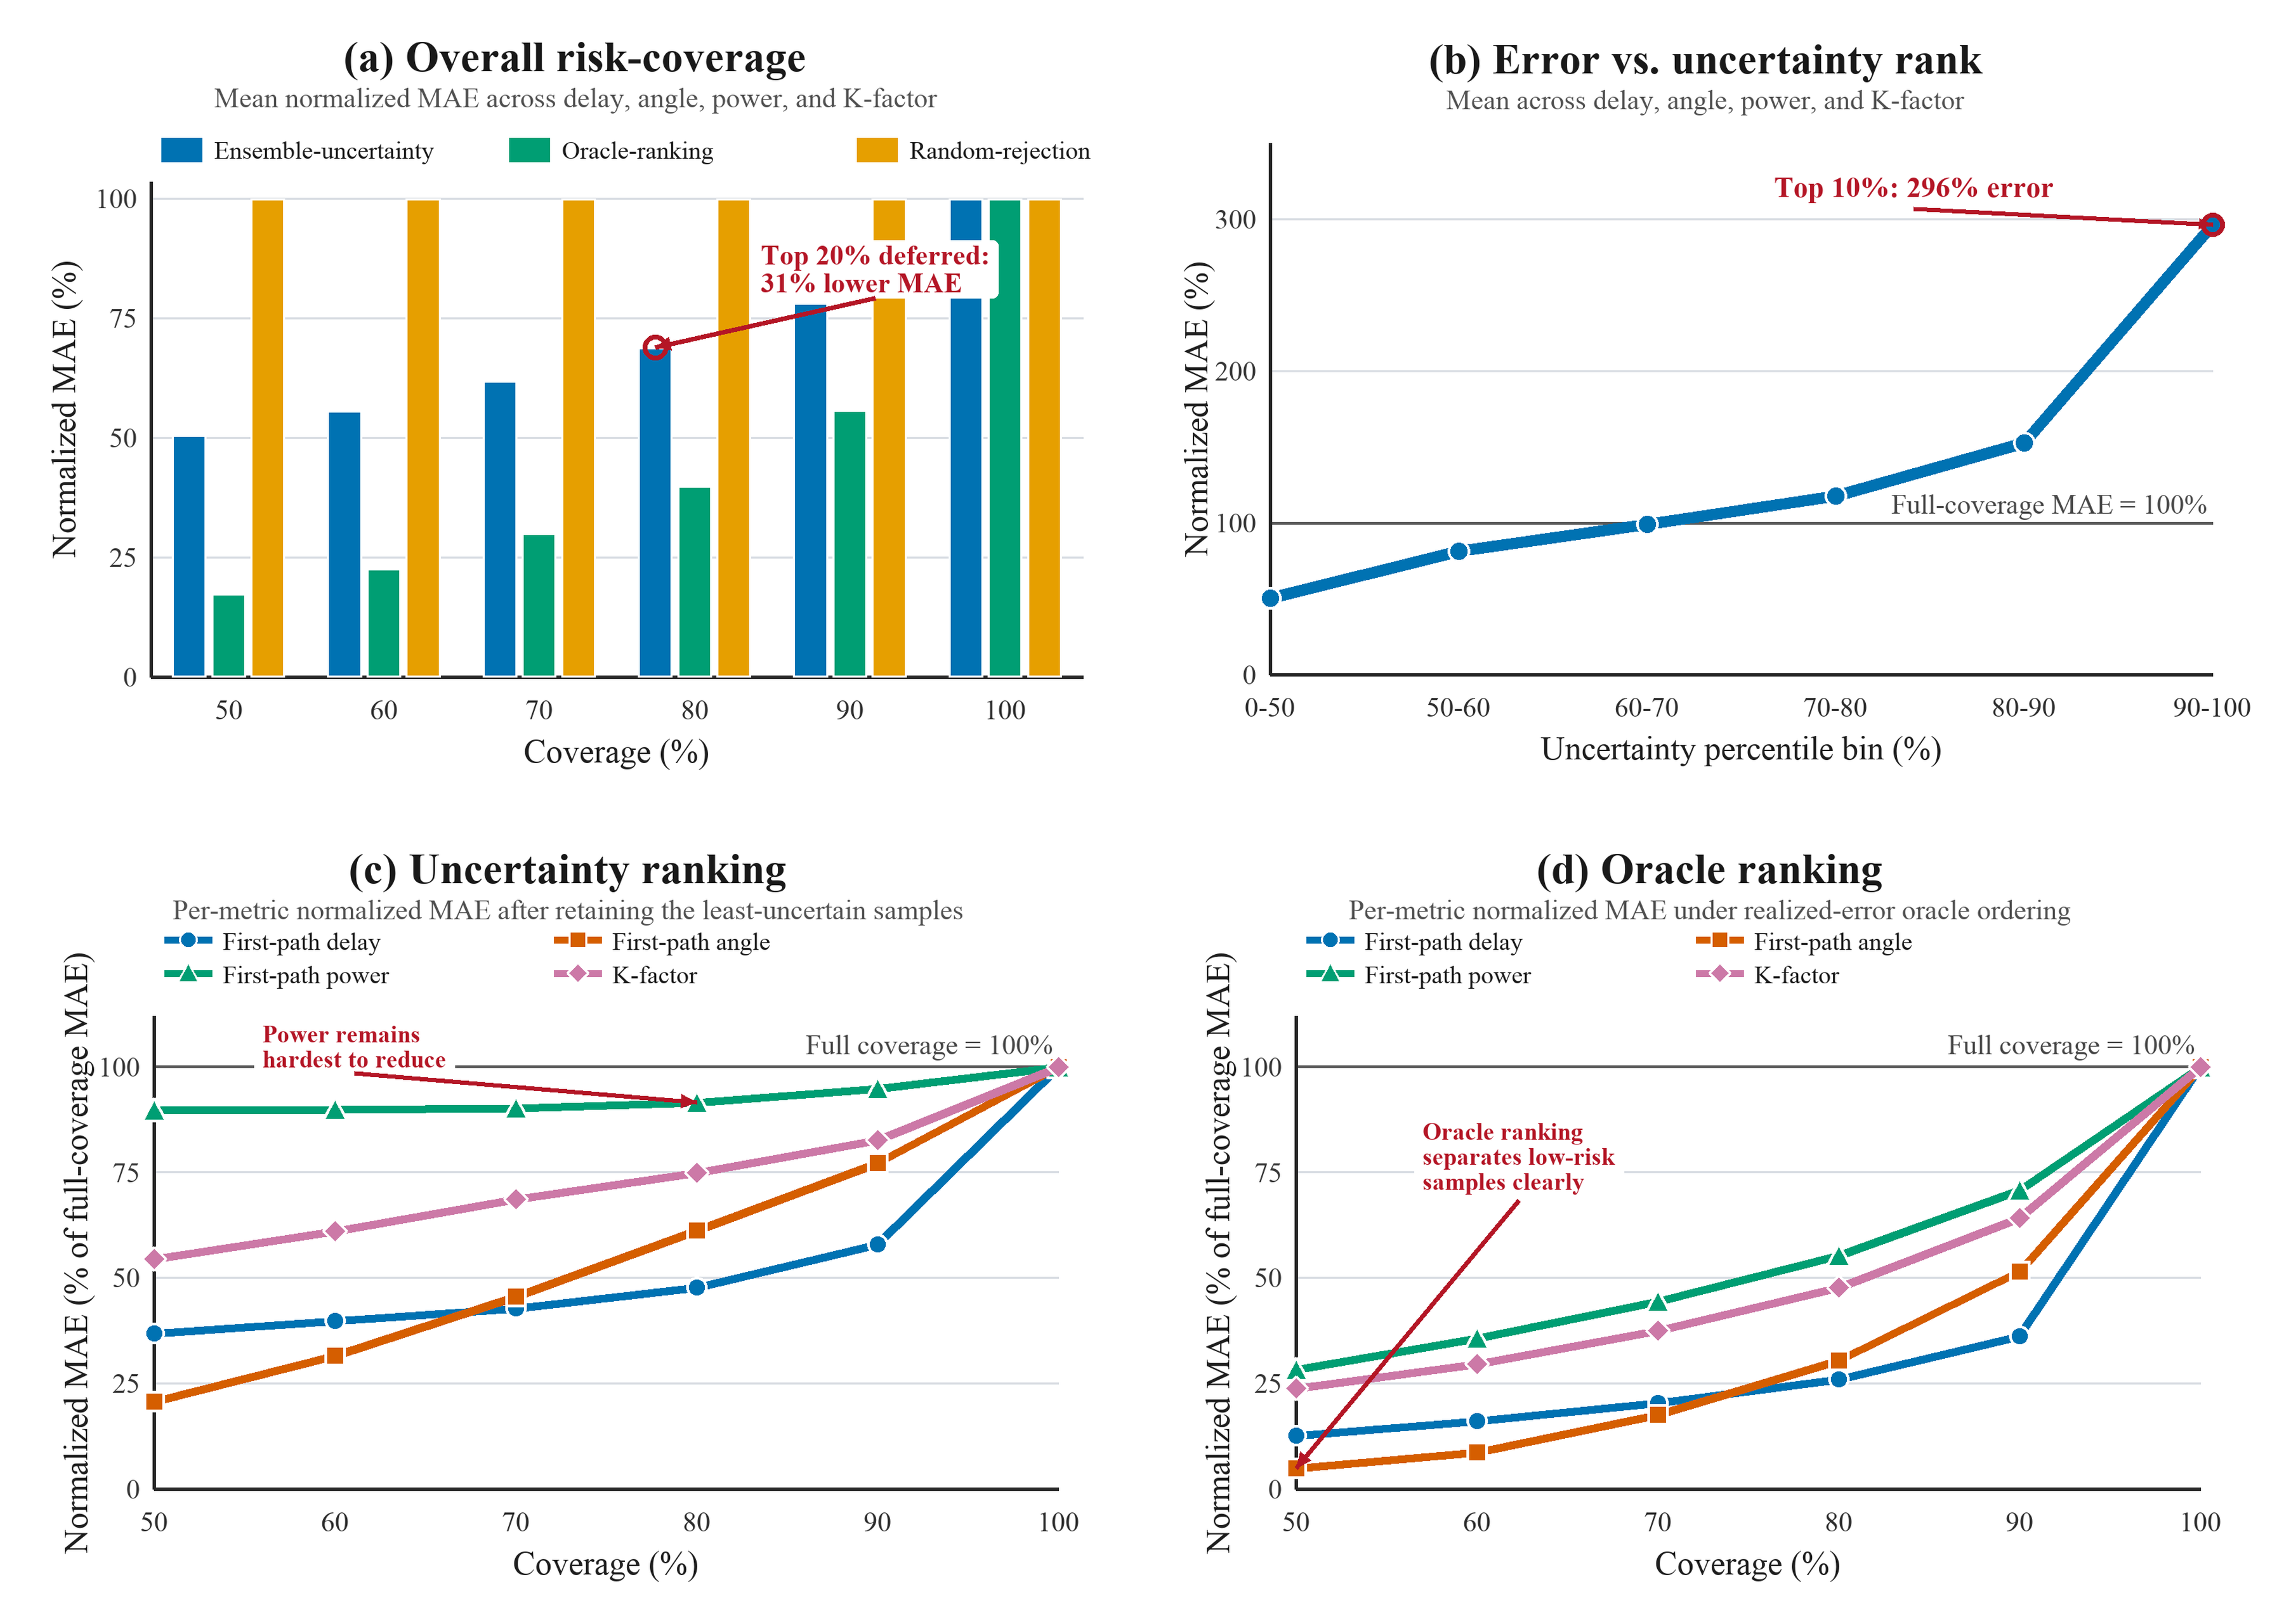
\includegraphics[width=\columnwidth]{figures/selective_prediction_four_panel.png}
\caption{Reliability-aware selective-prediction diagnostics. (a) Cross-metric normalized
risk--coverage comparison at discrete coverage levels for ensemble-uncertainty ranking,
oracle ranking, and random rejection. (b) Cross-metric normalized MAE versus
uncertainty-percentile bin; 100\% denotes the full-coverage MAE. (c) Per-metric
normalized MAE for first-path delay, angle, power, and $K$-factor under uncertainty
ranking. (d) The same per-metric normalized MAE under oracle ranking. All values are
normalized by the corresponding full-coverage MAE, and lower is better.}
\label{fig:nlos-selective-prediction}
\end{figure}

Figure~\ref{fig:nlos-selective-prediction} shows that ensemble disagreement usefully ranks prediction
risk across heterogeneous physical quantities. After normalizing each metric by its full-coverage
MAE and averaging delay, angle, power, and \(K\)-factor, deferring the highest-uncertainty 10\% and
20\% reduces retained-set error to about 78\% and 69\% of the full-coverage baseline, while random
rejection remains at 100\% in expectation. The bin-wise view is consistent: normalized error rises
from roughly 51\% for the least-uncertain half to 296\% for the highest-uncertainty decile. Although
the remaining gap to the oracle shows that disagreement is not perfectly calibrated, the improvement
over random rejection supports a practical policy: automatically emit low-uncertainty reports and
route deferred samples to additional sensing, paired-numerology fusion, or review. Panel (d) further
shows that the gain is strongest for delay and angle, remains useful for \(K\)-factor, and is weaker
for first-path power.
\subsection{Measured SISO Validation}

We evaluate the pipeline on the Wi-World RealData BUPT mobile-measurement scene
TXH1\_RX01. The acquisition settings in Table~\ref{tab:bupt-config} follow the official dataset
documentation~\cite{wiworldrealdata}. The receiver moves slowly along the measurement route, and
each MAT file covers approximately 0.1 s of a \(1\times1\) SISO link.

\begin{table}[H]
\centering
\caption{Measured-data acquisition, sampling hierarchy, and model input. The independent evaluation
unit is a MAT file; snapshots from the same MAT share one short-time measurement interval.}
\label{tab:bupt-config}
\scriptsize
\setlength{\tabcolsep}{3.0pt}
\renewcommand{\arraystretch}{1.05}
\textbf{Panel A: acquisition configuration}\par\vspace{2pt}
\begin{tabular}{p{0.34\columnwidth}p{0.59\columnwidth}}
\toprule
\textbf{Item} & \textbf{Setting} \\
\midrule
Scene & BUPT TXH1\_RX01; slowly moving receiver \\
Carrier / bandwidth & 3.7 GHz / 200 MHz \\
CIR sampling & 200 MHz; 5 ns delay interval \\
Sounding sequence & PN11; length 2047; 100 MSample/s \\
CIR record & 4094 taps; adjacent CIR interval 20.47 \(\mu\)s \\
MAT contents & Approximately 0.1 s; 4885 or 4886 CIRs \\
Transmitter & LB-20180 horn; 10.206 dBi gain \\
Receiver & SZ-3004000/P omnidirectional bicone; 0.952 dBi gain \\
Channel structure & \(1\times1\) SISO \\
\bottomrule
\end{tabular}

\vspace{4pt}
\textbf{Panel B: data hierarchy}\par\vspace{2pt}
\resizebox{\columnwidth}{!}{%
\begin{tabular}{lcl}
\toprule
\textbf{Level} & \textbf{Amount / size} & \textbf{Role} \\
\midrule
Complete route & \(\sim2997\) MAT / \(\sim900\) GB & Original data pool \\
Local medium pool & 400 MAT / 114.72 GiB & Complete MAT and context retained \\
Debug subset & 10 MAT / \(\sim2.9\) GiB & Pipeline verification; contained in the 60 MAT \\
Formal measured subset & 60 MAT / 17.21 GiB & 60 independent evaluation units \\
Model snapshots & \(60\times32=1920\) & Correlated within each MAT \\
\bottomrule
\end{tabular}}
\end{table}

The 60 formal MAT files are uniformly selected in time from the 400-file local pool. They span
17:45:09.200 to 17:49:58.300 on May 30, 2026, for a total of 289.1 s; the median interval between
selected MAT files is 4.7 s. Each MAT is treated as one approximate measurement location and one
independent evaluation unit. The 10 debug MAT files are included in these 60 files and therefore
must not be counted as 10 additional locations.

Each MAT contains approximately 4885 consecutive CIRs. We uniformly sample 32 snapshots over its
full 0.1 s interval, giving
\begin{equation}
N_{\mathrm{input}}=60\ \mathrm{MAT}\times32\
\frac{\mathrm{snapshots}}{\mathrm{MAT}}=1920\ \mathrm{CSI\ snapshots}.
\label{eq:measured-snapshot-count}
\end{equation}
The 1920 model inputs are not 1920 statistically independent measurement points: the 32 snapshots
within a MAT share the same short-time environment. Each snapshot is converted to 256 frequency
points over 200 MHz, with 781.25 kHz spacing, and represented by real and imaginary channels with
shape \((1,2,256)\). A complete MAT therefore produces an input tensor of shape
\((32,1,2,256)\), with a 1.28 \(\mu\)s unambiguous delay window.

The preprocessing pipeline reads the complex CIR, samples the 32 snapshots, computes their shared
mean power-delay profile (PDP), estimates the noise floor, and constructs one shared soft path mask.
The masked complex CIR is transformed by FFT, resampled to the 256-point frequency grid, corrected
for the fixed system-delay linear phase, and normalized by a per-snapshot common phase before forming
the SISO input. The shared mask threshold is
\begin{equation}
P_{\mathrm{th}}=
\max\!\left(P_{\mathrm{peak}}-25\ \mathrm{dB},
P_{\mathrm{noise}}+6\ \mathrm{dB}\right).
\label{eq:measured-soft-mask}
\end{equation}
Tap weights are zero below the noise floor, one above \(P_{\mathrm{th}}\), and smoothly interpolated
between these limits. Using the same mask for all 32 snapshots in a MAT prevents weak paths from
appearing or disappearing solely because of snapshot-level noise.

The detected first arrival contains both propagation delay and a fixed acquisition-system delay:
\begin{equation}
\tau_{\mathrm{detected}}=
\tau_{\mathrm{system}}+\tau_{\mathrm{propagation}}.
\label{eq:measured-system-delay}
\end{equation}
GNSS positions are successfully matched for 58 of the 60 MAT files. From these, 12 lower-envelope
geometric-LoS candidates are selected, and their median gives
\(\hat{\tau}_{\mathrm{system}}=6199.06\) ns, equivalent to 1239.81 samples at 200 MHz.
Across the candidates, the standard deviation is 37.53 ns, the median absolute deviation is
33.43 ns, and the range is 6161.30--6269.06 ns. We define the reference as the
\emph{PDP-derived calibrated first-arrival delay}
\begingroup
\setlength{\abovedisplayskip}{4pt}
\setlength{\belowdisplayskip}{4pt}
\setlength{\abovedisplayshortskip}{4pt}
\setlength{\belowdisplayshortskip}{4pt}
\begin{equation}
\widetilde{\tau}_{\mathrm{FA}}=
n_{\mathrm{first}}\times5\ \mathrm{ns}-6199.06\ \mathrm{ns}.
\label{eq:measured-calibrated-first-arrival}
\end{equation}
\endgroup
This wording is deliberate: the offset is estimated from automatically selected geometric-LoS
candidates rather than from an independent hardware calibration, so
\(\widetilde{\tau}_{\mathrm{FA}}\) is not strict ground truth.

Only two outputs have measurement-derived references in this experiment:
\(\widetilde{\tau}_{\mathrm{FA}}\) and RMS delay spread \(\tau_{\mathrm{RMS}}\), the latter obtained
from a classical PDP estimator. Other structured outputs, including absolute path power, physical ray
count, interaction count, and receiver-side angle, have no independent reference labels in this
measured subset. They may be generated by the model, but they are excluded from quantitative
accuracy claims. Table~\ref{tab:bupt-measured} therefore evaluates only the two supported delay
quantities.

System-delay calibration reduces first-arrival-delay MAE from 244.78 to 55.25 ns (77.4\%), reduces
the absolute bias from 244.78 to 51.22 ns, and raises Pearson correlation from 0.929 to 0.963. The
remaining negative bias indicates systematic underestimation, although the high correlation shows
that sample-to-sample variation is preserved. Importantly, the residual 55.25 ns is an end-to-end
discrepancy against an automatically constructed reference, rather than pure model error. In signed
form, it contains model, GNSS, first-path-detection, and system-delay-calibration terms. The median
reported RX-position standard deviations are approximately 8.2 m, 11.4 m, and 9.7 m along the
latitude, longitude, and height coordinates; as an order-of-magnitude reference, a 10 m range error
corresponds to about 33 ns of propagation delay. A weak physical first path may also fall below the
PDP detector threshold, causing a later reflection tens of nanoseconds away to be used as the
reference. Finally, the 12 calibration candidates themselves have a 33.43 ns MAD and span
6161.30--6269.06 ns. GNSS uncertainty also propagates into this offset estimate, so these terms are
not independent and the full 55.25 ns cannot be attributed to the predictor alone. For
\(\tau_{\mathrm{RMS}}\), soft-mask AWGN fine-tuning attains 15.941 ns MAE; AWGN training from scratch
gives the best overall result of 13.442 ns MAE, 16.008 ns RMSE, and \(r=0.891\).

\begin{table}[H]
\centering
\caption{Measured SISO delay results on BUPT. Panel A evaluates system-delay calibration for the
PDP-derived first-arrival reference; Panel B compares \(\tau_{\mathrm{RMS}}\) training and
preprocessing. Lower is better for MAE and RMSE; higher is better for Pearson \(r\).}
\label{tab:bupt-measured}
\scriptsize
\setlength{\tabcolsep}{3.0pt}
\renewcommand{\arraystretch}{1.08}
\textbf{Panel A: PDP-derived calibrated first arrival \(\widetilde{\tau}_{\mathrm{FA}}\)}\par\vspace{2pt}
\begin{tabular}{lcc}
\toprule
\textbf{Metric} & \shortstack{\textbf{Soft mask,}\textbf{uncalibrated}} &
\shortstack{\textbf{Soft mask,}\textbf{calibrated}} \\
\midrule
Reference mean (ns) & 758.02 & 758.02 \\
Prediction mean (ns) & 513.25 & 706.81 \\
MAE (ns) $\downarrow$ & 244.78 & \best{\relgain{55.25}} \\
Bias (ns) & $-244.78$ & \relgain{$-51.22$} \\
Pearson $r$ $\uparrow$ & 0.929 & \best{0.963} \\
\bottomrule
\end{tabular}

\vspace{5pt}
\textbf{Panel B: RMS delay spread \(\tau_{\mathrm{RMS}}\)}\par\vspace{2pt}
\resizebox{\columnwidth}{!}{%
\begin{tabular}{llccccc}
\toprule
\textbf{Training} & \textbf{BUPT input} & \textbf{Pred. mean} &
\textbf{MAE $\downarrow$} & \textbf{RMSE $\downarrow$} & \textbf{Bias} &
\textbf{Pearson $r$ $\uparrow$} \\
\midrule
Clean & Raw & 223.994 & 177.906 & 189.028 & $+177.906$ & 0.410 \\
AWGN fine-tuning & Raw & 141.609 & 95.896 & 115.063 & $+95.521$ & 0.423 \\
Clean & Soft mask & 95.016 & 48.929 & 66.988 & $+48.929$ & 0.548 \\
AWGN fine-tuning & Soft mask & 50.583 & 15.941 & 25.976 & \best{$+4.495$} & 0.563 \\
\rowcolor{modelblue}\textbf{AWGN from scratch} & \textbf{Soft mask} & \textbf{57.597} & \best{\relgain{13.442}} & \best{\relgain{16.008}} & \relgain{$+11.509$} & \best{\textbf{0.891}} \\
\bottomrule
\end{tabular}}
\end{table}

The measured-data experiment should be interpreted as an in-sample validation of preprocessing,
calibration, and delay transfer, not as a leakage-free generalization test. In particular, the
6199.06 ns offset is estimated from candidates drawn from the same 60-MAT evaluation subset.
An independent calibration route or direct hardware-delay measurement is needed before claiming
out-of-sample absolute-delay accuracy.

\subsection{Transfer to Downstream Wireless Tasks}

\begin{figure}[H]
\centering
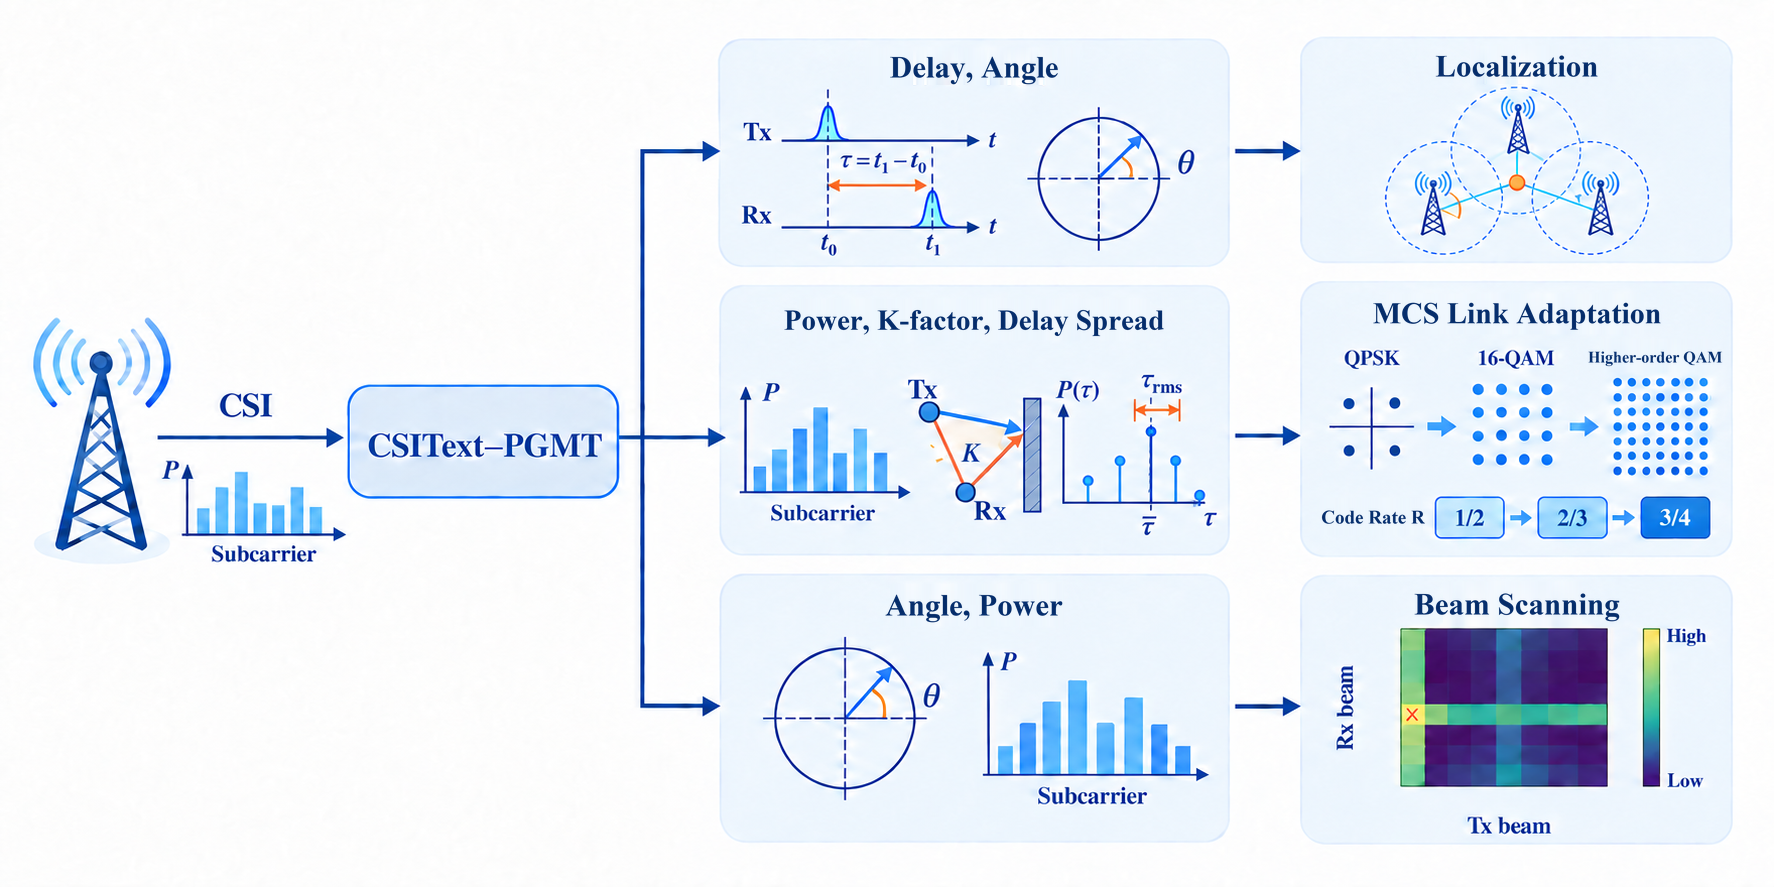
\includegraphics[width=0.98\columnwidth]{figures/csitext_pgmt_applications_english.png}
\caption{Representative downstream uses of the learned CSI representation and predicted propagation
attributes. The shared representation supports localization, MCS link adaptation, and transmit-beam
selection; the quantitative study additionally evaluates adaptive cyclic-prefix selection and
link-quality/outage prediction.}
\label{fig:downstream-applications}
\end{figure}

We further evaluate five downstream communication tasks to determine whether the learned CSI
representation is transferable to practical network decisions rather than being useful only for
channel reporting. Figure~\ref{fig:downstream-applications} summarizes the interface: downstream
heads receive either CSI features, the pretrained embedding, or the embedding augmented with
predicted propagation attributes. Whenever physics features are used, they are model predictions
rather than ground-truth test labels. The five tasks cover localization, cyclic-prefix (CP) control,
link-quality and outage prediction, MCS adaptation, and transmit-beam selection.

\subsubsection{Two-Dimensional Localization}

For localization, the transmitter and receiver coordinates define the relative-position target
\((\Delta x,\Delta y)=(x_{\mathrm{RX}}-x_{\mathrm{TX}},
y_{\mathrm{RX}}-y_{\mathrm{TX}})\). A regression head maps the CSI representation to this two-dimensional
offset. This task tests whether the representation retains spatial information that is not explicitly
required by the language report. Table~\ref{tab:downstream-localization} shows that augmenting a
trainable CSI encoder with frozen predicted physics gives the lowest mean and median errors and the
largest fractions within 5 and 10 m. The result indicates that the predicted LoS state, delay, and
angular structure provide useful geometric cues beyond a generic language backbone.

\begin{table}[H]
\centering
\caption{Two-dimensional localization on the common test split. Lower is better for mean and median
error; higher is better for distance-threshold accuracy. Underlining marks the best result. The final
row compares the highlighted model with the best of the three language-model baselines (red:
improvement; blue: degradation); threshold accuracies are reported as percentage-point differences.}
\label{tab:downstream-localization}
\scriptsize
\setlength{\tabcolsep}{2.8pt}
\resizebox{\columnwidth}{!}{%
\begin{tabular}{lcccc}
\toprule
Method & Mean (m) $\downarrow$ & Median (m) $\downarrow$ & $\leq5$ m (\%) $\uparrow$ & $\leq10$ m (\%) $\uparrow$ \\
\midrule
\rowcolor{modelblue}\textbf{Scratch + frozen physics} & \best{\textbf{34.15}} & \best{\textbf{10.67}} & \best{\textbf{34.04}} & \best{\textbf{49.02}} \\
Scratch & 47.07 & 20.13 & 13.36 & 35.32 \\
Pretrained embedding & 65.06 & 54.46 & 0.88 & 4.02 \\
Pretrained embedding + physics & 36.91 & 12.04 & 29.70 & 48.20 \\
\midrule
Qwen3.5-2B, full fine-tuning & 100.90 & 101.17 & 0.20 & 0.48 \\
DeepSeek-R1-Qwen3-8B, frozen & 100.79 & 101.09 & 0.16 & 0.50 \\
InternLM3-8B, frozen & 80.07 & 78.95 & 0.86 & 3.10 \\
\midrule
\rowcolor{gainrow}\textbf{Rel. vs. best LLM} & \relgain{57.3\%} & \relgain{86.5\%} & \relgain{33.18 pp} & \relgain{45.92 pp} \\
\bottomrule
\end{tabular}}
\end{table}

\subsubsection{Adaptive Cyclic-Prefix Selection}

For each link, offline ray delays and powers define the shortest candidate CP whose protection
interval contains at least 99\% of the multipath energy. A classifier then selects among the
candidate CP durations from the CSI representation and predicted multipath attributes. The objective
is to avoid an unsafe short CP while also avoiding excessive overhead from an unnecessarily long CP.
Table~\ref{tab:downstream-cp} shows a clear tradeoff: pretrained features alone minimize energy
outside the chosen CP, whereas adding predicted physics yields the highest classification accuracy
and the lowest over-selection rate. Thus, the learned representation supports both reliability-aware
and efficiency-aware CP control.

\begin{table}[H]
\centering
\caption{Adaptive CP selection. Under-selection chooses a CP shorter than the oracle, whereas
over-selection chooses a longer CP. Lower outside-energy values are safer. Underlining marks the
best result for each directed metric. The final row compares the highlighted model with the best of
the three language-model baselines (red: improvement; blue: degradation); predicted CP is
descriptive and is therefore omitted from the relative comparison.}
\label{tab:downstream-cp}
\scriptsize
\setlength{\tabcolsep}{2.0pt}
\resizebox{\columnwidth}{!}{%
\begin{tabular}{lcccccc}
\toprule
Method & Acc. $\uparrow$ & Under $\downarrow$ & Over $\downarrow$ & Pred. CP (ns) & Mean out $\downarrow$ & P95 out $\downarrow$ \\
\midrule
\rowcolor{modelblue}\textbf{Pretrained embedding + physics} & \best{\textbf{70.92\%}} & \textbf{15.92\%} & \best{\textbf{13.16\%}} & \textbf{215.17} & \textbf{4.54\%} & \textbf{9.35\%} \\
Scratch & 51.86\% & 27.32\% & 20.82\% & 189.93 & 6.51\% & 55.51\% \\
Pretrained embedding & 58.62\% & \best{12.22\%} & 29.16\% & 283.01 & \best{2.27\%} & \best{5.21\%} \\
Scratch + frozen physics & 67.76\% & 14.90\% & 17.34\% & 221.40 & 3.57\% & 5.39\% \\
\midrule
Qwen3.5-2B, full fine-tuning & 51.76\% & 19.72\% & 28.52\% & 290.20 & 2.80\% & 10.18\% \\
InternLM3-8B, frozen + CSI & 55.58\% & 21.24\% & 23.18\% & 208.43 & 6.24\% & 57.31\% \\
DeepSeek-8B, frozen + CSI & 58.30\% & 15.74\% & 25.96\% & 247.43 & 3.27\% & 11.37\% \\
\midrule
\rowcolor{gainrow}\textbf{Rel. vs. best LLM} & \relgain{21.6\%} & \relloss{1.1\%} & \relgain{43.2\%} & --- & \relloss{62.1\%} & \relgain{8.2\%} \\
\bottomrule
\end{tabular}}
\end{table}

\subsubsection{Link Quality and Outage Prediction}

The link-quality task estimates received power and decides whether a link remains operational under
the specified noise condition. It therefore tests whether the learned power, LoS, and multipath cues
are sufficiently calibrated for reliability-oriented decisions. As shown in
Table~\ref{tab:downstream-outage}, the CSI2TEXT-PGMT total-power head gives the lowest power MAE,
while all methods exceed 98.9\% outage accuracy and F1. The language baselines obtain slightly higher
binary scores but incur larger power errors, showing that an accurate outage decision does not by
itself guarantee a faithful continuous link-quality estimate.

\begin{table}[H]
\centering
\caption{Link-quality and outage prediction. Lower is better for power MAE; higher is better for
outage accuracy and F1. Underlining marks the best result. The final row compares the highlighted
model with the best of the three language-model baselines (red: improvement; blue: degradation).}
\label{tab:downstream-outage}
\scriptsize
\setlength{\tabcolsep}{2.6pt}
\resizebox{\columnwidth}{!}{%
\begin{tabular}{llccc}
\toprule
Method & Training & Power MAE $\downarrow$ & Outage acc. $\uparrow$ & Outage F1 $\uparrow$ \\
\midrule
\rowcolor{modelblue}\textbf{\model{}} & \textbf{Total-power head} & \best{\textbf{2.1098 dB}} & \textbf{98.92\%} & \textbf{98.90\%} \\
DeepSeek-R1-Qwen3-8B & Frozen + adapter/head & 3.0165 dB & 99.52\% & 99.51\% \\
InternLM3-8B-Instruct & Frozen + adapter/head & 2.8207 dB & 99.52\% & 99.51\% \\
Qwen3.5-2B & Full fine-tuning & 2.4603 dB & \best{99.56\%} & \best{99.55\%} \\
\midrule
\rowcolor{gainrow}\multicolumn{2}{l}{\textbf{Rel. vs. best LLM}} & \relgain{14.2\%} & \relloss{0.6\%} & \relloss{0.7\%} \\
\bottomrule
\end{tabular}}
\end{table}

\subsubsection{MCS Link Adaptation}

For MCS adaptation, each sample combines the CSI representation, transmit power, and predicted
propagation features. Effective-SNR and calibrated BLER constraints define the highest feasible MCS,
including an outage class when no MCS satisfies the target. The classifier must therefore maximize
spectral efficiency without violating the reliability constraint. Table~\ref{tab:downstream-mcs}
shows that the scratch CSI2TEXT-PGMT configuration reaches 99.05\% accuracy, only 0.53\% BLER
violations, and 99.90\% of oracle goodput. This demonstrates that the structured CSI interface can
support near-oracle link adaptation without relying on a large language decoder at inference.

\begin{table}[H]
\centering
\caption{MCS link adaptation under calibrated BLER constraints. Lower is better for MCS MAE and
BLER violation; higher is better for accuracy, goodput ratio, and outage recall. The final row
compares the highlighted model with the best of the three language-model baselines (red:
improvement; blue: degradation).}
\label{tab:downstream-mcs}
\scriptsize
\setlength{\tabcolsep}{2.0pt}
\resizebox{\columnwidth}{!}{%
\begin{tabular}{lccccc}
\toprule
Method & Acc. $\uparrow$ & MCS MAE $\downarrow$ & BLER viol. $\downarrow$ & Goodput $\uparrow$ & Outage recall $\uparrow$ \\
\midrule
\rowcolor{modelblue}\textbf{Scratch} & \best{\textbf{99.05\%}} & \best{\textbf{0.0098}} & \best{\textbf{0.53\%}} & \best{\textbf{99.90\%}} & \textbf{99.49\%} \\
Pretrained embedding & 91.80\% & 0.1016 & 3.56\% & 96.67\% & 95.94\% \\
Pretrained embedding + physics & 92.20\% & 0.0948 & 4.40\% & 97.11\% & 95.21\% \\
Scratch + frozen physics & 98.07\% & 0.0321 & 1.38\% & 99.63\% & 98.02\% \\
\midrule
Qwen3.5-2B & 95.44\% & 0.0458 & 1.22\% & 98.54\% & \best{99.59\%} \\
DeepSeek-R1-Qwen3-8B & 94.56\% & 0.0544 & 4.76\% & 98.00\% & 98.29\% \\
InternLM3-8B & 94.98\% & 0.0504 & 2.46\% & 98.60\% & 98.62\% \\
\midrule
\rowcolor{gainrow}\textbf{Rel. vs. best LLM} & \relgain{3.8\%} & \relgain{78.6\%} & \relgain{56.6\%} & \relgain{1.3\%} & \relloss{0.1\%} \\
\bottomrule
\end{tabular}}
\end{table}

\subsubsection{Adaptive Transmit-Beam Search}

The beam task reconstructs the 64 candidate beams of an $8\times8$ UPA and uses the beam with the
largest average received gain as the oracle label. A 64-class head predicts the best transmit-beam
index from the full CSI representation. This evaluates whether the representation preserves the
directional information required for beam management. Table~\ref{tab:downstream-beam} shows that
scratch training augmented with frozen predicted physics gives the strongest overall result: 87.84\%
Top-1 accuracy, 96.52\% Top-3 accuracy, and only 1.33 dB mean gain loss. The improvement is largest
for NLoS links, where indirect multipath cues are particularly valuable.

\begin{table}[H]
\centering
\caption{Full-CSI transmit-beam prediction over 64 UPA beams. Lower is better for gain loss; higher
is better for all other metrics. Underlining marks the best result. The final row compares the
highlighted model with the best of the three language-model baselines (red: improvement; blue:
degradation).}
\label{tab:downstream-beam}
\scriptsize
\setlength{\tabcolsep}{1.8pt}
\resizebox{\columnwidth}{!}{%
\begin{tabular}{lccccccc}
\toprule
Method & Top-1 & Top-3 & $\leq1$ dB & Mean $\downarrow$ & P90 $\downarrow$ & LoS & NLoS \\
\midrule
\rowcolor{modelblue}\textbf{Scratch + frozen physics} & \best{\textbf{87.84\%}} & \best{\textbf{96.52\%}} & \best{\textbf{89.92\%}} & \best{\textbf{1.33}} & \best{\textbf{1.11}} & \textbf{98.80\%} & \best{\textbf{76.88\%}} \\
Pretrained embedding & 87.10\% & 95.40\% & 89.40\% & 1.57 & 1.60 & 98.68\% & 75.52\% \\
Pretrained embedding + physics & 87.02\% & 95.20\% & 89.10\% & 1.62 & 2.05 & 98.80\% & 75.24\% \\
Scratch & 86.04\% & 96.28\% & 88.38\% & 1.65 & 2.75 & \best{98.88\%} & 73.20\% \\
\midrule
Qwen3.5-2B & 77.30\% & 91.10\% & 80.35\% & 2.53 & 10.79 & 92.50\% & 62.10\% \\
InternLM3-8B-Instruct & 77.60\% & 90.15\% & 81.25\% & 2.51 & 10.05 & 92.60\% & 62.60\% \\
DeepSeek-R1-Qwen3-8B & 49.00\% & 76.15\% & 51.65\% & 8.04 & 25.72 & 66.50\% & 31.50\% \\
\midrule
\rowcolor{gainrow}\textbf{Rel. vs. best LLM} & \relgain{13.2\%} & \relgain{5.9\%} & \relgain{10.7\%} & \relgain{47.0\%} & \relgain{89.0\%} & \relgain{6.7\%} & \relgain{22.8\%} \\
\bottomrule
\end{tabular}}
\end{table}

Across the five tasks, no single feature choice dominates every secondary metric, but the results
consistently show that CSI-native representations and predicted propagation attributes provide a
compact and effective interface for network control. In particular, physics assistance is most useful
for geometry- and multipath-sensitive decisions, while lightweight CSI heads can match or exceed
direct language-model baselines at substantially lower inference cost.


\section{Conclusion}

We presented CSI-to-language conversion as a grounded inference problem rather than open-ended
generation. CSI2TEXT-PGMT first recovers a typed channel state using configuration-aware,
target-specific physical representations and then converts the corrected record into an auditable
description through deterministic verbalization. The resulting reports are structurally complete and
substantially more accurate than direct learned decoders on the underlying numerical quantities. The
generalization, split-sensitivity, and observation-noise studies further show that the decisive challenge
is not fluent language generation, but the recovery of indirect multipath structure, especially under
NLoS propagation. This factorization provides an interpretable interface for wireless-channel
analytics while making both successes and failures traceable to explicit physical fields. Future work
should extend the framework to measured channels, hardware impairments, calibrated uncertainty, and
more expressive multipath-aware objectives.

\begin{thebibliography}{99}

\bibitem{alkhateeb2019deepmimo}
Ahmed Alkhateeb. DeepMIMO: A generic deep learning dataset for millimeter wave and massive
MIMO applications. \emph{arXiv preprint arXiv:1902.06435}, 2019.

\bibitem{chen2018gradnorm}
Zhao Chen, Vijay Badrinarayanan, Chen-Yu Lee, and Andrew Rabinovich. GradNorm: Gradient
normalization for adaptive loss balancing in deep multitask networks. In \emph{Proceedings of the
35th International Conference on Machine Learning}, volume 80, pages 794--803, 2018.

\bibitem{deepseek2025r1}
DeepSeek-AI. DeepSeek-R1: Incentivizing reasoning capability in LLMs via reinforcement learning.
\emph{arXiv preprint arXiv:2501.12948}, 2025.

\bibitem{ferrand2023charting}
Paul Ferrand, Maxime Guillaud, Christoph Studer, and Olav Tirkkonen. Wireless channel charting:
Theory, practice, and applications. \emph{arXiv preprint arXiv:2304.08095}, 2023.

\bibitem{fleury1999sage}
Bernard H. Fleury, Martin Tschudin, Rainer Heddergott, Dirk Dahlhaus, and Klaus I. Pedersen.
Channel parameter estimation in mobile radio environments using the SAGE algorithm. \emph{IEEE
Journal on Selected Areas in Communications}, 17(3):434--450, 1999.

\bibitem{guo2017calibration}
Chuan Guo, Geoff Pleiss, Yu Sun, and Kilian Q. Weinberger. On calibration of modern neural
networks. In \emph{Proceedings of the 34th International Conference on Machine Learning},
volume 70, pages 1321--1330, 2017.

\bibitem{internlm2025}
InternLM Team. InternLM3-8B-Instruct Model Card. Hugging Face model repository, 2025.
\url{https://huggingface.co/internlm/internlm3-8b-instruct}.

\bibitem{keya2026wirelesssense}
Mahmuda Keya, Sneh Pillai, Jiawei Yuan, Kai Zeng, and Long Jiao. WirelessSenseLLM: Zero-shot
human activity understanding by bridging wireless signals and human language. \emph{arXiv preprint
arXiv:2605.14070}, 2026.

\bibitem{liu2024wifo}
Boxun Liu, Shijian Gao, Xuanyu Liu, Xiang Cheng, and Liuqing Yang. WiFo: Wireless foundation
model for channel prediction. \emph{arXiv preprint arXiv:2412.08908}, 2024.

\bibitem{orekondy2023winert}
Tribhuvanesh Orekondy, Pratik Kumar, Shreya Kadambi, Hao Ye, Joseph Soriaga, and Arash
Behboodi. WiNeRT: Towards neural ray tracing for wireless channel modelling and differentiable
simulations. In \emph{International Conference on Learning Representations}, 2023.

\bibitem{palhares2025csi2vec}
Victoria Palhares, Sueda Taner, and Christoph Studer. CSI2Vec: Towards a universal CSI feature
representation for positioning and channel charting. \emph{arXiv preprint arXiv:2506.05237}, 2025.

\bibitem{qwen2025}
Qwen Team. Qwen3 Technical Report. \emph{arXiv preprint arXiv:2505.09388}, 2025.

\bibitem{qwen2026}
Qwen Team. Qwen3.5-2B Model Card. Hugging Face model repository, 2026.
\url{https://huggingface.co/Qwen/Qwen3.5-2B}.

\bibitem{radford2021clip}
Alec Radford, Jong Wook Kim, Chris Hallacy, Aditya Ramesh, Gabriel Goh, Sandhini Agarwal,
Girish Sastry, Amanda Askell, Pamela Mishkin, Jack Clark, Gretchen Krueger, and Ilya Sutskever.
Learning transferable visual models from natural language supervision. In \emph{Proceedings of the
38th International Conference on Machine Learning}, volume 139, pages 8748--8763, 2021.

\bibitem{roy1989esprit}
Richard Roy and Thomas Kailath. ESPRIT-estimation of signal parameters via rotational invariance
techniques. \emph{IEEE Transactions on Acoustics, Speech, and Signal Processing},
37(7):984--995, 1989.

\bibitem{schmidt1986music}
Ralph O. Schmidt. Multiple emitter location and signal parameter estimation. \emph{IEEE
Transactions on Antennas and Propagation}, 34(3):276--280, 1986.

\bibitem{scholak2021picard}
Torsten Scholak, Nathan Schucher, and Dzmitry Bahdanau. PICARD: Parsing incrementally for
constrained auto-regressive decoding from language models. In \emph{Proceedings of the 2021
Conference on Empirical Methods in Natural Language Processing}, pages 9895--9901, 2021.

\bibitem{studer2018charting}
Christoph Studer, Said Medjkouh, Emre Gonultas, Tom Goldstein, and Olav Tirkkonen. Channel
charting: Locating users within the radio environment using channel state information. \emph{IEEE
Access}, 6:47682--47698, 2018.

\bibitem{rayverse2025}
UNIC Lab. RayVerse: A large-scale urban radio-propagation dataset generated using ray tracing,
2025. \url{https://github.com/UNIC-Lab/RayVerse}. Accessed July 27, 2026.

\bibitem{wei2026wifi2cap}
Tzu-Ti Wei, Chu-Yu Huang, Yu-Chee Tseng, and Jen-Jee Chen. WiFi2Cap: Semantic action
captioning from Wi-Fi CSI via limb-level semantic alignment. \emph{arXiv preprint
arXiv:2603.22690}, 2026.

\bibitem{wiworldrealdata}
Wi-World. \emph{RealData Dataset README\_Chinese}. Official dataset documentation.

\bibitem{zhu2024physics}
Guangxu Zhu, Yuanming Sun, and Kaibin Ji. Physics-informed generalizable wireless channel
modeling with segmentation and deep learning: Fundamentals, methodologies, and challenges.
\emph{arXiv preprint arXiv:2401.01288}, 2024.

\bibitem{zou2026rfgpt}
Hang Zou, Yu Tian, Bohao Wang, Lina Bariah, Samson Lasaulce, Chongwen Huang, and Merouane
Debbah. RF-GPT: Teaching AI to see the wireless world. \emph{arXiv preprint
arXiv:2602.14833}, 2026.

\end{thebibliography}

\clearpage
\appendices

\section{Target Construction and Physical Scope}

This appendix defines the simulator-derived quantities represented by the structured record. These
definitions establish annotation semantics and reproducibility; they are not additional learned
components.

\subsection{Valid Paths, First Path, and Absolute Power}

Let $\mathcal P$ be the finite set of paths retained by the D2Los/RayVerse export:
\[
\mathcal P=\{p\mid P_p^{\mathrm{dBW}}\ \text{and}\ \tau_p\ \text{are finite}\}.
\]
No additional relative-power threshold is applied. The first path is the earliest retained path,
\[
p^\star=\arg\min_{p\in\mathcal P}\tau_p,
\qquad
\tau_1=\tau_{p^\star},
\qquad
p_1^{\mathrm{dBW}}=P_{p^\star}^{\mathrm{dBW}}.
\]
Simulator path loss $L_p^{\mathrm{dB}}$ is converted to received-path power using the fixed transmit
power $P_{\mathrm{tx}}=23$ dBm:
\[
P_p^{\mathrm{dBW}}=P_{\mathrm{tx}}^{\mathrm{dBm}}-L_p^{\mathrm{dB}}-30.
\]
The first-path-power target is therefore an absolute value under this transmit-power assumption, not
a per-link relative value. This definition motivates the raw-scale bypass in the model: per-example
standardization benefits representation learning but removes the amplitude scale required by the power
head.

\subsection{Delay Spread, Angular Spread, and the K-Factor Label}

With linear power $P_p=10^{P_p^{\mathrm{dBW}}/10}$, the delay-spread label is the power-weighted
RMS spread,
\[
\bar\tau=\frac{\sum_pP_p\tau_p}{\sum_pP_p},
\qquad
\sigma_\tau=\sqrt{\frac{\sum_pP_p(\tau_p-\bar\tau)^2}{\sum_pP_p}}.
\]
Angular spread uses circular statistics. With $w_p=P_p/\sum_qP_q$,
\[
R=\left|\sum_pw_pe^{j\theta_p}\right|,
\qquad
\sigma_\theta=\frac{180}{\pi}\sqrt{-2\log(\operatorname{clip}(R,10^{-6},1))}.
\]
For a LoS link with residual reflected paths, the simulator-derived ray-power-ratio label is
\[
K_{\mathrm{dB}}=10\log_{10}\frac{P_0}{\sum_{p\geq1}P_p}.
\]
NLoS links are assigned $-20$ dB, and a LoS link with no residual path is assigned 30 dB. This is
a derived label based on the retained ray powers, not a multi-snapshot Rician $K$ estimator.

\subsection{Path and Reflection-Interaction Semantics}

The supplied CSI dataset contains reflected propagation paths and does not include diffraction or
scattering components. Consequently, the stored interaction counts can be interpreted as reflection
interactions for this dataset. Let $c_p$ be the stored reflection-interaction count of retained path $p$.
The record distinguishes
\[
n_{\mathrm{refl}}=\sum_{p\in\mathcal P}\min(c_p,9),
\qquad
n_{\mathrm{rpath}}=\sum_{p\in\mathcal P}\mathbf 1[c_p>0],
\]
where $n_{\mathrm{refl}}$ is the total encoded reflection-interaction count and
$n_{\mathrm{rpath}}$ is the number of reflected paths. A single path may contain multiple reflections,
so these quantities are related but not identical. Path count is read from the export without a new
top-$K$ truncation. An audit of 742,818 links from 20 source files found one to five saved paths per
link; five is an empirical ceiling of the supplied exports, not a universal physical limit.

\subsection{Observability Boundaries}

The retained spatial aperture is on the transmitter side and only one receive element is supplied.
Frequency-dependent phase supports delay inference, and the transmitter array supports
transmitter-side spatial structure. Receiver-side AoA is therefore treated as a supervised
cross-domain target learned from correlations among transmitter-side beam-frequency CSI, multipath
structure, and ray-traced geometry. It must not be interpreted as a directly measured receive-array
beam direction. For the same reason, classical receive-array estimators such as MUSIC, ESPRIT, and
Bartlett are not commensurate baselines for the receiver-side angle labels in this dataset.

\section{Implementation and Evaluation Details}

\subsection{Encoder, Alignment, and Prediction Heads}

ULA inputs use an antenna-axis FFT and group four adjacent beams per token. UPA inputs use a
row-column two-dimensional FFT and $2\times2$ local beam patches. Real and imaginary components
are concatenated. The shared encoder combines a linear frequency projection, depthwise-pointwise
convolution, adaptive average/max summaries, feature-wise configuration modulation, beam-position
embeddings, and carrier/frequency encodings.

The Transformer has six layers, hidden width 384, six attention heads, and a 1,536-dimensional
feed-forward block. The fused $[\mathrm{CLS}]$ and masked-mean representation is projected to a
normalized 256-dimensional CSI embedding. Descriptions use a 300-token vocabulary with maximum
length 48. A three-layer, four-head Transformer of width 256 produces the text embedding. Semantic
prototype keys combine environment, LoS/NLoS status, path richness, delay and angular regimes,
$K$ bin, and reflection statistics; classes with fewer than five training samples are discarded.

For completeness, the alignment loss retains the full symmetric pairwise InfoNCE form used in the
initial draft. For two normalized embedding families $z_a$ and $z_b$ in a minibatch of size $N$,
\begin{align}
\mathcal L_{a,b}=-\frac{1}{2N}\sum_{i=1}^{N}\bigg[&
\log\frac{\exp\!\left((z_a^i)^\top z_b^i/T\right)}
{\sum_{j=1}^{N}\exp\!\left((z_a^i)^\top z_b^j/T\right)} \notag\\[-2pt]
&+\log\frac{\exp\!\left((z_b^i)^\top z_a^i/T\right)}
{\sum_{j=1}^{N}\exp\!\left((z_b^i)^\top z_a^j/T\right)}\bigg].
\label{eq:symmetric-infonce}
\end{align}
The initial temperature is $T=0.07$. Equation~\ref{eq:symmetric-infonce} is instantiated for
CSI--text, CSI--prototype, and text--prototype pairs. Thus both retrieval directions contribute to
each pairwise term rather than treating one embedding family as a fixed one-way target.

Temporal quantities use frequency- and delay-domain features, angular quantities use circular
representations, and absolute power combines the standardized representation with the raw-scale
bypass. Reflection-interaction count and reflected-path count use separate prediction heads because
one path may contain multiple reflection interactions.

\subsection{Loss Weights and Optimization}

\begin{table}[t]
\centering
\caption{Loss configuration used for the main model.}
\label{tab:appendix-loss}
\scriptsize
\setlength{\tabcolsep}{2pt}
\resizebox{\columnwidth}{!}{%
\begin{tabular}{lcc}
\toprule
Group & Term & Weight \\
\midrule
Alignment & CSI--text / CSI--prototype / text--prototype & 1.0 / 1.0 / 1.0 \\
Representation & semantic / attribute / auxiliary physics & 0.5 / 0.1 / 0.005 \\
$K$ factor & strong-bin classifier / within-bin position & 0.5 / 0.1 \\
First delay & normalized / raw / fused raw & 0.08 / 0.001 / 0.02 \\
First delay & bin / position / consistency / tail underestimate & 0.02 / 0.01 / 0.01 / 0.01 \\
Delay spread & raw / bin / within-bin position & 0.0005 / 0.03 / 0.008 \\
LoS delay & regression / nonnegative / consistency & 0.05 / 0.005 / 0.005 \\
Angles & LoS / first path / NLoS first path & 0.05 / 0.02 / 0.01 \\
First power & bin / position; NLoS multiplier & 0.03 / 0.1; 2.0 \\
Reflections & classifier / regression; NLoS multiplier & 0.02 / 0.01; 1.0 \\
\bottomrule
\end{tabular}}
\end{table}

Table~\ref{tab:appendix-loss} records the main loss configuration. The optional relational training
regularizer has weight zero in the reported main runs; record-level correction is applied after
prediction.

Models train for 100 epochs with AdamW, batch size 128, initial learning rate $3\times10^{-4}$,
weight decay $10^{-2}$, five epochs of linear warm-up, and cosine decay to $10^{-5}$. Every epoch
traverses all 40,000 main training examples. Retaining the final incomplete minibatch gives 313
minibatches per epoch and 31,300 scheduled optimizer steps. Unless stated otherwise, seeds are 0, 1,
and 2, and error bars are sample standard deviations. The balanced main model has 28,938,178
trainable parameters. A run uses one NVIDIA RTX 4090 with 23.6 GB memory, PyTorch 2.5.1 with
CUDA 12.1, and no automatic mixed precision; a representative run takes approximately 5.5 hours.

\subsection{Data Cohorts and Split Construction}

\begin{table*}[t]
\centering
\caption{Core cohorts and isolation rules.}
\label{tab:cohort-core}
\scriptsize
\setlength{\tabcolsep}{4pt}
\begin{tabular}{lccc>{\centering\arraybackslash}p{5.2cm}}
\toprule
Cohort & Purpose & Train/test & LoS/NLoS & Isolation and use \\
\midrule
SRC-400K & source pool & 400K & original & no train/test split; source for subsequent sampling \\
MAIN-50K-v1 & main experiment & 40K/10K & 20K/20K; 5K/5K & 78 training and 19 test maps with zero group-ID overlap; full model, conventional baselines, and architectural ablations \\
SD-50K & scenario isolation & 40K/10K & balanced & map-, spatial-block-, UE-position-, and group-disjoint scenario evaluation \\
\bottomrule
\end{tabular}
\end{table*}

\begin{table*}[t]
\centering
\caption{Specialized cohorts. Reflection labels are available unless otherwise noted.}
\label{tab:cohort-specialized}
\scriptsize
\setlength{\tabcolsep}{3.5pt}
\begin{tabular}{lccc>{\centering\arraybackslash}p{4.5cm}}
\toprule
Cohort & Purpose & Train/test & Balance & Isolation or label status \\
\midrule
CORR-100K & relational correction & 80K/20K & balanced & zero shared links/samples; 97 shared maps \\
RPATH-100K & reflected-path extension & 80K/20K & 13,628/86,372 & random split; map/link isolation not audited; reflected-path labels reconstructed and verified \\
DD-100K-v2 & decoder training & 40K/1K & balanced & zero shared links/samples; 97 shared maps; reconstructed labels \\
COST-50K-RPATH-v2 & cost benchmark & 40K/10K & balanced & zero shared links/samples; 97 shared maps \\
Noise-Augment-50K & noise study & 40K/10K & balanced & zero shared links/samples; 97 shared maps \\
\bottomrule
\end{tabular}
\end{table*}

All cohorts originate from the 400,000-link source pool. Tables~\ref{tab:cohort-core} and
\ref{tab:cohort-specialized} transcribe the cohort plan used across the main, stress-test, decoder,
correction, extension, and cost studies. Cohort-qualified names prevent numerical differences across
independently sampled experiments from being interpreted as contradictory estimates on one fixed
test set.

For complete map-disjoint evaluation, 78 of 97 source maps form a 321,644-example training parent
and 19 maps form a 78,356-example evaluation parent. Balanced subsets are sampled only within
their parents: 20,000 LoS and 20,000 NLoS links for training, and 5,000 of each for evaluation.
Ordered group IDs, maps, map-qualified spatial blocks, and exact UE positions are checked for empty
intersection. The spatial-block protocol has no guard band, so complete map separation remains the
stronger scenario-disjoint test.

The 400,000-link source pool contains 53,577 LoS and 346,423 NLoS examples. The exact test-map
IDs are
\begin{multline*}
\{1,7,15,17,21,22,25,28,30,34,\\
50,53,54,55,81,89,96,98,99\}.
\end{multline*}
all remaining map IDs are training-only. The balanced-subset samplers use seed 23,441 for training
and seed 23,442 for evaluation.

Split provenance is verified at four levels. First, the ordered training and evaluation group-ID lists
are compared directly. Second, each group is expanded to its map ID, map-qualified spatial-block ID,
and exact UE position, and every train--test intersection is required to be empty. Third, the ordered
10,000-example evaluation list stored with each run is compared with the audited evaluation manifest.
Fourth, each checkpoint record is bound to the exact training manifest and sampling seed used to fit
it. SHA-256 hashes of the complete ordered ID lists, rather than hashes of unordered sets or row counts,
are retained in the machine-readable audit. These checks detect three leakage failures that a row-count
or class-balance check cannot: (i) cohorts with the same LoS/NLoS balance but shared physical links,
(ii) different links sampled from a map that should have been held out in its entirety, and (iii) a
checkpoint trained from a manifest different from the one associated with the reported evaluation
table.

\subsection{Text Metrics and Tolerance Definitions}

\begin{table}[t]
\centering
\caption{Field-specific numerical tolerance accuracy on the balanced MAIN-50K-v1 evaluation split
(mean $\pm$ sample standard deviation over three seeds).}
\label{tab:field-tolerance-complete}
\scriptsize
\setlength{\tabcolsep}{3pt}
\begin{tabular}{lc}
\toprule
Field and tolerance & Accuracy $\uparrow$ \\
\midrule
Path count ($\pm1$) & $0.9533\pm0.0061$ \\
First-path delay ($\pm50$ ns) & $0.9451\pm0.0032$ \\
First-path angle ($\pm15^\circ$) & $0.6841\pm0.0102$ \\
First-path power ($\pm5$ dB) & $0.6436\pm0.0430$ \\
$K$ factor ($\pm3$ dB) & $0.7971\pm0.0302$ \\
Delay spread ($\pm50$ ns) & $0.9700\pm0.0003$ \\
Angular spread ($\pm15^\circ$) & $0.7907\pm0.0716$ \\
LoS delay ($\pm50$ ns) & $0.9915\pm0.0012$ \\
LoS angle ($\pm15^\circ$) & $0.9972\pm0.0007$ \\
Reflection-interaction count ($\pm1$) & $0.6562\pm0.0031$ \\
\bottomrule
\end{tabular}
\end{table}

Predicted and reference descriptions are parsed into typed slots. Categorical fields use accuracy and
macro-F1. Numeric-slot F1 measures whether required values are present. Hallucination is the fraction
of predicted numeric slots unsupported by the reference schema. Numerical tolerance accuracy checks
whether a present value is within 50 ns for delay, $15^\circ$ for angle, 5 dB for first-path power,
3 dB for $K$, and one count for path or reflection fields. Composite factuality is the macro average
of categorical accuracies, numeric-slot F1, numerical tolerance accuracy, and one minus hallucination.
It is not sentence exact match. Raw MAE remains necessary because the tolerance thresholds are
application choices.

The tolerance table complements MAE by exposing the fraction of fields that meet application-scale
error bands. It also shows why one aggregate numerical-accuracy value is insufficient: LoS-specific
geometry is highly reliable, whereas first-path power and reflection multiplicity remain harder.

\subsection{Baselines and Inference Settings}

Physics baselines include flattened CSI with an MLP, a CNN, PDP/IFFT features with an MLP, a
Transformer without specialized branches, and independent single-task heads on the same CSI
encoder. Direct learned decoders map the CSI encoder representation to a learned soft prefix for
Qwen3-1.7B, Qwen3.5-2B, InternLM3-8B, or DeepSeek-R1-Qwen3-8B. These decoders learn to emit
the same record schema but do not use the target-specific physical heads. The four decoder results are
single trained runs; their missing error bars must not be interpreted as zero variance.

\section{Additional Experimental Evidence}

This section adds protocols and evidence not already tabulated in the main paper. Main-text AWGN,
cross-configuration, split-sensitivity, propagation-regime, and language-alignment tables are not
repeated.

\subsection{Complete Main-Model Aggregate Performance}

\begin{table}[t]
\centering
\caption{Complete aggregate performance of CSI2TEXT-PGMT-MAIN-50K on the balanced main split
(mean $\pm$ sample standard deviation over three seeds).}
\label{tab:complete-main-fields}
\scriptsize
\setlength{\tabcolsep}{3pt}
\begin{tabular}{lc}
\toprule
Target & Result \\
\midrule
Environment accuracy (\%) $\uparrow$ & $100.00\pm0.00$ \\
LoS/NLoS accuracy (\%) $\uparrow$ & $99.58\pm0.11$ \\
Path-count MAE $\downarrow$ & $0.215\pm0.056$ \\
First-path delay MAE (ns) $\downarrow$ & $21.91\pm0.30$ \\
First-path angle MAE ($^\circ$) $\downarrow$ & $16.61\pm0.56$ \\
First-path power MAE (dB) $\downarrow$ & $4.34\pm0.27$ \\
$K$-factor MAE (dB) $\downarrow$ & $2.15\pm0.04$ \\
Delay-spread MAE (ns) $\downarrow$ & $11.30\pm0.26$ \\
Angular-spread MAE ($^\circ$) $\downarrow$ & $9.72\pm0.47$ \\
LoS-delay MAE (ns) $\downarrow$ & $8.83\pm0.55$ \\
LoS-angle MAE ($^\circ$) $\downarrow$ & $1.33\pm0.17$ \\
NLoS first-delay MAE (ns) $\downarrow$ & $40.66\pm1.58$ \\
NLoS first-angle MAE ($^\circ$) $\downarrow$ & $35.88\pm0.96$ \\
Reflection-interaction-count MAE $\downarrow$ & $1.032\pm0.019$ \\
Reflected-path-count MAE $\downarrow$ & $0.086\pm0.005$ \\
\bottomrule
\end{tabular}
\end{table}

Table~\ref{tab:complete-main-fields} restores the full-label view from the initial draft. The
first-path delay is aligned to the current MAIN-50K-v1 result, $21.91$ ns; it should not be confused
with the separately sampled COST-50K-RPATH-v2 value reported in the inference-cost subsection.

The categorical fields are nearly saturated and path-count error remains small, but the complete
view reveals a pronounced propagation-regime asymmetry: LoS delay and angle errors are
$8.83$ ns and $1.33^\circ$, whereas the corresponding NLoS values are $40.66$ ns and
$35.88^\circ$. The two reflection quantities are intentionally separate: one counts encoded
reflection events, while the other counts paths containing at least one reflection. The NLoS
delay/angle entries were derived seed-wise on this exactly balanced cohort from
$E_{\mathrm{NLoS}}=2E_{\mathrm{all}}-E_{\mathrm{LoS}}$; this identity must not be reused for an
imbalanced cohort.

\subsection{Cross-Configuration Protocol and Extended Fields}

The frequency-transfer model is trained jointly on $N_f\in\{64,96,192,256\}$ and evaluated on
$N_f=128$, which is excluded from fitting. This tests interpolation to a held-out sampling
configuration after phase-preserving resampling; it does not establish arbitrary transfer across carrier
frequency or bandwidth. The mixed-array model is trained on UPA-$8\times8$ and ULA-64 and
evaluated on aligned held-out UPA-$4\times4$, UPA-$16\times4$, and ULA-32 groups. Directional
ULA transfer is evaluated separately in both $64\rightarrow32$ and $32\rightarrow64$ directions.
The complete per-setting results are summarized in the main paper; the principal protocol safeguard
is that held-out array groups do not reuse fitted physical links.

\subsection{Paired Multi-Numerology Expert Fusion}
\label{sec:paired-numerology-fusion}

The main cross-configuration experiment asks whether one CSI observation acquired under an unseen
frequency-sampling configuration can be interpreted without configuration-specific fine-tuning. We
additionally consider an assisted setting in which two CSI observations of the same physical link are
available under different numerologies. This setting represents multi-numerology sounding or
coordinated measurements in which complementary frequency resolutions provide different evidence
about the same propagation channel. Because both observations are available at inference time, this
experiment complements rather than replaces the single-input held-out-$N_f$ evaluation.

Let $(\mathbf H^{(a)},\mathbf c^{(a)})$ and $(\mathbf H^{(b)},\mathbf c^{(b)})$ denote the paired
observations. The shared encoder produces configuration-aware representations $\mathbf z_c^{(a)}$
and $\mathbf z_c^{(b)}$, from which the two experts generate structured predictions
$\hat{\mathbf y}^{(a)}$ and $\hat{\mathbf y}^{(b)}$. A lightweight gate assigns sample-dependent
continuous weights,
\[
\begin{aligned}
\bigl[g_a,g_b\bigr]&=\operatorname{softmax}\!\left(
G\!\left[\mathbf z_c^{(a)};\mathbf z_c^{(b)};\right.\right.\\[-2pt]
&\hspace{5.7em}\left.\left.\mathbf c^{(a)};\mathbf c^{(b)}\right]\right),
\qquad g_a+g_b=1,
\end{aligned}
\]
and forms the fused record
\[
\hat{\mathbf y}_{\mathrm{soft}}
=g_a\hat{\mathbf y}^{(a)}+g_b\hat{\mathbf y}^{(b)}.
\]
Unlike unconditional direct fusion, the gate can vary the contribution of each numerology for every
link. We compare soft weighting with hard expert selection and an A/B hard gate. The optional gate
changes only the structured physical prediction; relational correction and deterministic verbalization
remain unchanged.

\begin{table}[t]
\centering
\caption{Paired multi-numerology delay fusion from the same expert-gating experiment. Only fusion
outputs are shown. Lower is better, and underlining marks the best fusion result in each column.}
\label{tab:paired-numerology-fusion}
\small
\setlength{\tabcolsep}{6pt}
\resizebox{\columnwidth}{!}{%
\begin{tabular}{lcccc}
\toprule
\textbf{Fusion method} & \textbf{$96{+}128$ first delay $\downarrow$} &
\textbf{$96{+}128$ LoS delay $\downarrow$} &
\textbf{$128{+}192$ first delay $\downarrow$} &
\textbf{$128{+}192$ LoS delay $\downarrow$} \\
\midrule
\textbf{Direct fusion} & 63.14 & 32.05 & 49.79 & 26.17 \\
\textbf{A/B hard gate} & 63.31 & 24.70 & \best{32.73} & \best{19.90} \\
\textbf{Hard expert gate} & 60.45 & 25.04 & 35.28 & 21.69 \\
\textbf{Soft expert gate} & \best{57.58} & \best{23.24} & 37.67 & 20.53 \\
\bottomrule
\end{tabular}}
\end{table}

For the $N_f=96+128$ pair, soft expert gating reduces first-delay MAE from 63.14 to 57.58 ns
and LoS-delay MAE from 32.05 to 23.24 ns relative to direct fusion. Averaged over the four
pair--target entries in Table~\ref{tab:paired-numerology-fusion}, its MAE is 34.76 ns, compared
with 42.79 ns for direct fusion, 35.16 ns for the A/B hard gate, and 35.62 ns for hard expert
selection. Soft weighting therefore provides the strongest overall balance among the evaluated
fusion strategies.

The improvement is not uniform. For $N_f=128+192$, the A/B hard gate gives the lowest fused
first-delay and LoS-delay errors, while soft weighting remains close. More generally, paired fusion
cannot guarantee improvement when one numerology already provides substantially stronger evidence
than the other. The result supports adaptive multi-numerology fusion as an optional extension under
paired-input availability, rather than as a requirement of the main CSI-to-text pipeline. A separately
trained calibrated confidence-fallback variant reduces signed prediction bias, but it is retained as a
calibration diagnostic and is not mixed into this controlled expert-gating comparison.

\subsection{Language Alignment and Relational Correction}
\label{sec:appendix-language-shift}

\begin{table}[t]
\centering
\caption{Language-alignment ablation under scenario-disjoint evaluation. Lower is better for MAE;
higher is better for reflection accuracy. Underlining marks the best value in each row.}
\label{tab:scenario-language-ablation}
\scriptsize
\setlength{\tabcolsep}{3.0pt}
\resizebox{\columnwidth}{!}{%
\begin{tabular}{lcccc}
\toprule
\textbf{Metric} & \textbf{Full} & \textbf{No CSI--text} &
\textbf{No text--prototype} & \textbf{Physics only} \\
\midrule
\textbf{First-delay MAE (ns) $\downarrow$} & \cellcolor{modelblue}\best{39.3698} & 39.8403 & 40.9318 & 40.1218 \\
\textbf{First-delay LoS MAE (ns) $\downarrow$} & \cellcolor{modelblue}\best{19.8347} & 20.9726 & 22.1455 & 21.4466 \\
\textbf{First-delay NLoS MAE (ns) $\downarrow$} & \cellcolor{modelblue}\best{58.0109} & 58.8105 & 59.8201 & 58.8984 \\
\textbf{LoS-delay MAE (ns) $\downarrow$} & \cellcolor{modelblue}\best{17.6445} & 20.2644 & 19.3338 & 21.4869 \\
\textbf{LoS-angle MAE ($^\circ$) $\downarrow$} & \cellcolor{modelblue}\best{2.2555} & 2.3383 & 2.3435 & 3.4443 \\
\textbf{First-angle LoS MAE ($^\circ$) $\downarrow$} & \cellcolor{modelblue}\best{3.7392} & 3.9504 & 3.9118 & 4.3980 \\
\textbf{First-angle NLoS MAE ($^\circ$) $\downarrow$} & \cellcolor{modelblue}41.4775 & 40.6324 & 42.2838 & \best{40.3674} \\
\textbf{Path-count MAE $\downarrow$} & \cellcolor{modelblue}\best{0.1935} & 0.2051 & 0.2505 & 0.3267 \\
\textbf{Reflection accuracy $\uparrow$} & \cellcolor{modelblue}\best{0.5388} & 0.5213 & 0.5310 & 0.5314 \\
\textbf{Delay-spread MAE (ns) $\downarrow$} & \cellcolor{modelblue}\best{17.7460} & 17.9922 & 18.2041 & 17.8470 \\
\textbf{$K$-factor MAE (dB) $\downarrow$} & \cellcolor{modelblue}3.3551 & 3.3279 & 3.3932 & \best{3.2915} \\
\textbf{First-power MAE (dB) $\downarrow$} & \cellcolor{modelblue}5.5425 & 5.4669 & 5.5787 & \best{5.3613} \\
\textbf{Azimuth-spread MAE ($^\circ$) $\downarrow$} & \cellcolor{modelblue}8.7741 & 9.6889 & 8.1116 & \best{7.8690} \\
\bottomrule
\end{tabular}}
\end{table}

The matched language-alignment results retained in the main paper use the current reported values;
the obsolete Appendix J table from the earlier draft is intentionally not reproduced. All ablation
variants retain direct physical supervision and the same deterministic verbalizer, so removing
semantic alignment need not cause a general collapse. The supported conclusion is localized:
alignment improves selected semantic and reflection-structure attributes but is not uniformly beneficial
for every fully supervised regressand.

The scenario-disjoint results localize the generalization benefit. Full alignment is best for all
reported delay quantities, LoS geometry, path count, reflection accuracy, and delay spread. Relative
to physics-only training, it reduces LoS-delay MAE by 17.9\%, LoS-angle MAE by 34.5\%, and
path-count MAE by 40.8\%. Text--prototype removal produces the largest delay degradation among the
two pairwise removals, indicating that coarse propagation prototypes help preserve temporal structure
outside the training scenarios. The result is not uniform: physics-only training remains better for
NLoS first-angle, $K$ factor, first-path power, and azimuth spread. Language alignment therefore acts
as a structured semantic regularizer, not as a universal replacement for target-specific physical
supervision.

\begin{table}[t]
\centering
\caption{Language-alignment ablation under clean-to-moderate complex AWGN. Lower is better for
physical MAE; higher is better for numerical tolerance accuracy. Uncertainty is shown where supplied.}
\label{tab:awgn-language-ablation-high}
\scriptsize
\setlength{\tabcolsep}{2.1pt}
\resizebox{\columnwidth}{!}{%
\begin{tabular}{llccc}
\toprule
\textbf{Condition} & \textbf{Model} & \textbf{First delay $\downarrow$} &
\textbf{First angle $\downarrow$} & \textbf{First power $\downarrow$} \\
\midrule
\rowcolor{modelblue}Clean & \textbf{Full} & $\best{25.974\pm0.344}$ & $\best{18.844\pm0.404}$ & $5.116\pm0.349$ \\
 & \textbf{No CSI--text} & 27.319 & 20.366 & 5.155 \\
 & \textbf{No text--prototype} & 27.916 & 20.706 & 4.876 \\
 & \textbf{Physics only} & 27.181 & 19.980 & \best{4.788} \\
\midrule
\rowcolor{modelblue}30 dB & \textbf{Full} & $\best{72.697\pm0.401}$ & $\best{23.101\pm0.844}$ & $\best{4.564\pm0.004}$ \\
 & \textbf{No CSI--text} & $77.509\pm0.235$ & $24.548\pm0.052$ & $4.888\pm0.003$ \\
 & \textbf{No text--prototype} & $83.644\pm0.090$ & $24.619\pm0.009$ & $4.862\pm0.014$ \\
 & \textbf{Physics only} & $85.775\pm0.240$ & $24.409\pm0.088$ & $4.567\pm0.002$ \\
\midrule
\rowcolor{modelblue}20 dB & \textbf{Full} & $\best{86.112\pm0.960}$ & $\best{24.292\pm0.711}$ & $\best{4.351\pm0.002}$ \\
 & \textbf{No CSI--text} & $89.023\pm0.289$ & $25.445\pm0.046$ & $4.745\pm0.003$ \\
 & \textbf{No text--prototype} & $95.650\pm0.413$ & $26.076\pm0.065$ & $4.787\pm0.372$ \\
 & \textbf{Physics only} & $103.020\pm0.319$ & $25.495\pm0.065$ & $4.461\pm0.006$ \\
\bottomrule
\end{tabular}}
\vspace{2pt}

\resizebox{\columnwidth}{!}{%
\begin{tabular}{llccc}
\toprule
\textbf{Condition} & \textbf{Model} & \textbf{$K$ factor $\downarrow$} &
\textbf{Refl. MAE $\downarrow$} & \textbf{Numeric acc. $\uparrow$} \\
\midrule
\rowcolor{modelblue}Clean & \textbf{Full} & $2.084\pm0.124$ & $\best{1.018\pm0.014}$ & $0.7405\pm0.0057$ \\
 & \textbf{No CSI--text} & 2.545 & 1.091 & 0.8360 \\
 & \textbf{No text--prototype} & \best{1.928} & 1.083 & 0.8438 \\
 & \textbf{Physics only} & 2.036 & 1.091 & \best{0.8477} \\
\midrule
\rowcolor{modelblue}30 dB & \textbf{Full} & $2.142\pm0.125$ & $\best{1.180\pm0.006}$ & $0.6927\pm0.0065$ \\
 & \textbf{No CSI--text} & $2.342\pm0.008$ & $1.201\pm0.000$ & $0.7972\pm0.0006$ \\
 & \textbf{No text--prototype} & $\best{1.930\pm0.006}$ & $1.192\pm0.003$ & $0.7976\pm0.0003$ \\
 & \textbf{Physics only} & $2.101\pm0.004$ & $1.202\pm0.002$ & $\best{0.8053\pm0.0010}$ \\
\midrule
\rowcolor{modelblue}20 dB & \textbf{Full} & $2.612\pm0.118$ & $\best{1.232\pm0.011}$ & $0.6491\pm0.0082$ \\
 & \textbf{No CSI--text} & $2.676\pm0.010$ & $1.240\pm0.004$ & $0.7579\pm0.0006$ \\
 & \textbf{No text--prototype} & $3.070\pm0.009$ & $1.307\pm0.004$ & $0.7387\pm0.0006$ \\
 & \textbf{Physics only} & $\best{2.335\pm0.006}$ & $1.250\pm0.002$ & $\best{0.7746\pm0.0007}$ \\
\bottomrule
\end{tabular}}
\end{table}

\begin{table}[t]
\centering
\caption{Language-alignment ablation under severe complex AWGN. Metric conventions match
Table~\ref{tab:awgn-language-ablation-high}.}
\label{tab:awgn-language-ablation-low}
\scriptsize
\setlength{\tabcolsep}{2.1pt}
\resizebox{\columnwidth}{!}{%
\begin{tabular}{llccc}
\toprule
\textbf{Condition} & \textbf{Model} & \textbf{First delay $\downarrow$} &
\textbf{First angle $\downarrow$} & \textbf{First power $\downarrow$} \\
\midrule
\rowcolor{modelblue}10 dB & \textbf{Full} & $\best{100.231\pm1.727}$ & $\best{25.123\pm0.786}$ & $5.377\pm0.576$ \\
 & \textbf{No CSI--text} & $101.013\pm0.212$ & $25.778\pm0.055$ & $4.814\pm0.015$ \\
 & \textbf{No text--prototype} & $107.434\pm0.269$ & $30.381\pm0.046$ & $5.248\pm0.023$ \\
 & \textbf{Physics only} & $120.664\pm0.467$ & $27.374\pm0.089$ & $\best{4.760\pm0.007}$ \\
\midrule
\rowcolor{modelblue}0 dB & \textbf{Full} & $\best{209.288\pm12.315}$ & $\best{32.296\pm1.919}$ & $17.692\pm0.076$ \\
 & \textbf{No CSI--text} & $209.599\pm0.669$ & $33.194\pm0.115$ & $18.059\pm0.053$ \\
 & \textbf{No text--prototype} & $222.284\pm0.419$ & $35.155\pm0.145$ & $17.598\pm0.005$ \\
 & \textbf{Physics only} & $209.656\pm0.610$ & $37.217\pm0.077$ & $\best{15.375\pm0.021}$ \\
\bottomrule
\end{tabular}}
\vspace{2pt}

\resizebox{0.92\columnwidth}{!}{%
\begin{tabular}{llccc}
\toprule
\textbf{Condition} & \textbf{Model} & \textbf{$K$ factor $\downarrow$} &
\textbf{Refl. MAE $\downarrow$} & \textbf{Numeric acc. $\uparrow$} \\
\midrule
\rowcolor{modelblue}10 dB & \textbf{Full} & $\best{5.494\pm0.582}$ & $\best{1.326\pm0.009}$ & $0.5622\pm0.0101$ \\
 & \textbf{No CSI--text} & $5.874\pm0.018$ & $1.332\pm0.006$ & $0.6845\pm0.0008$ \\
 & \textbf{No text--prototype} & $10.128\pm0.034$ & $1.344\pm0.003$ & $0.6425\pm0.0004$ \\
 & \textbf{Physics only} & $6.322\pm0.005$ & $1.427\pm0.002$ & $\best{0.7036\pm0.0001}$ \\
\midrule
\rowcolor{modelblue}0 dB & \textbf{Full} & $\best{19.855\pm0.659}$ & $2.384\pm0.178$ & $0.3393\pm0.0218$ \\
 & \textbf{No CSI--text} & $21.525\pm0.052$ & $2.446\pm0.002$ & $0.4684\pm0.0004$ \\
 & \textbf{No text--prototype} & $21.946\pm0.004$ & $2.412\pm0.003$ & $0.4702\pm0.0005$ \\
 & \textbf{Physics only} & $20.390\pm0.009$ & $\best{2.211\pm0.003}$ & $\best{0.5005\pm0.0003}$ \\
\bottomrule
\end{tabular}}
\end{table}

Across every tested SNR, Full gives the lowest first-delay and first-angle MAE. At 30, 20, and
10 dB, its first-delay error is respectively 15.2\%, 16.4\%, and 16.9\% lower than physics-only
training. Removing text--prototype alignment causes a larger delay penalty than removing CSI--text
alignment over most noisy conditions, supporting a robustness role for coarse propagation prototypes.
Full alignment also gives the lowest reflection MAE from clean through 10 dB, although physics-only
training becomes better at 0 dB. Power, $K$, and aggregate numerical tolerance accuracy retain
attribute-specific trade-offs, and physics-only training has the highest reported numerical accuracy.
The robust claim is therefore localized: semantic alignment stabilizes temporal, angular, and
reflection-structure representations under corruption, but does not improve every raw-scale or
tolerance-aggregated quantity.

The LoS identity $\tau_1=\tau_{\mathrm{LoS}}$ follows from the ray-tracing semantics. An audit of
84,464 LoS links from ten source files found exact equality at $10^{-6}$ ns tolerance. On a
representative seed-0 correction cohort, the raw first-path and LoS-delay heads have MAEs of 7.9958
and 6.4781 ns. Replacing both emitted slots with the dedicated LoS-delay estimate gives 6.4781 ns for
both fields on the same mask, reducing emitted first-delay error by 1.5177 ns while leaving LoS-delay
error unchanged. This is a post-processing diagnostic, not evidence that the raw neural head improved:
known identities can remove contradictions, but cannot repair unrelated physical quantities.

\subsection{Selective Prediction and Uncertainty Coverage}
\label{sec:selective-prediction}

\begin{figure}[H]
\centering
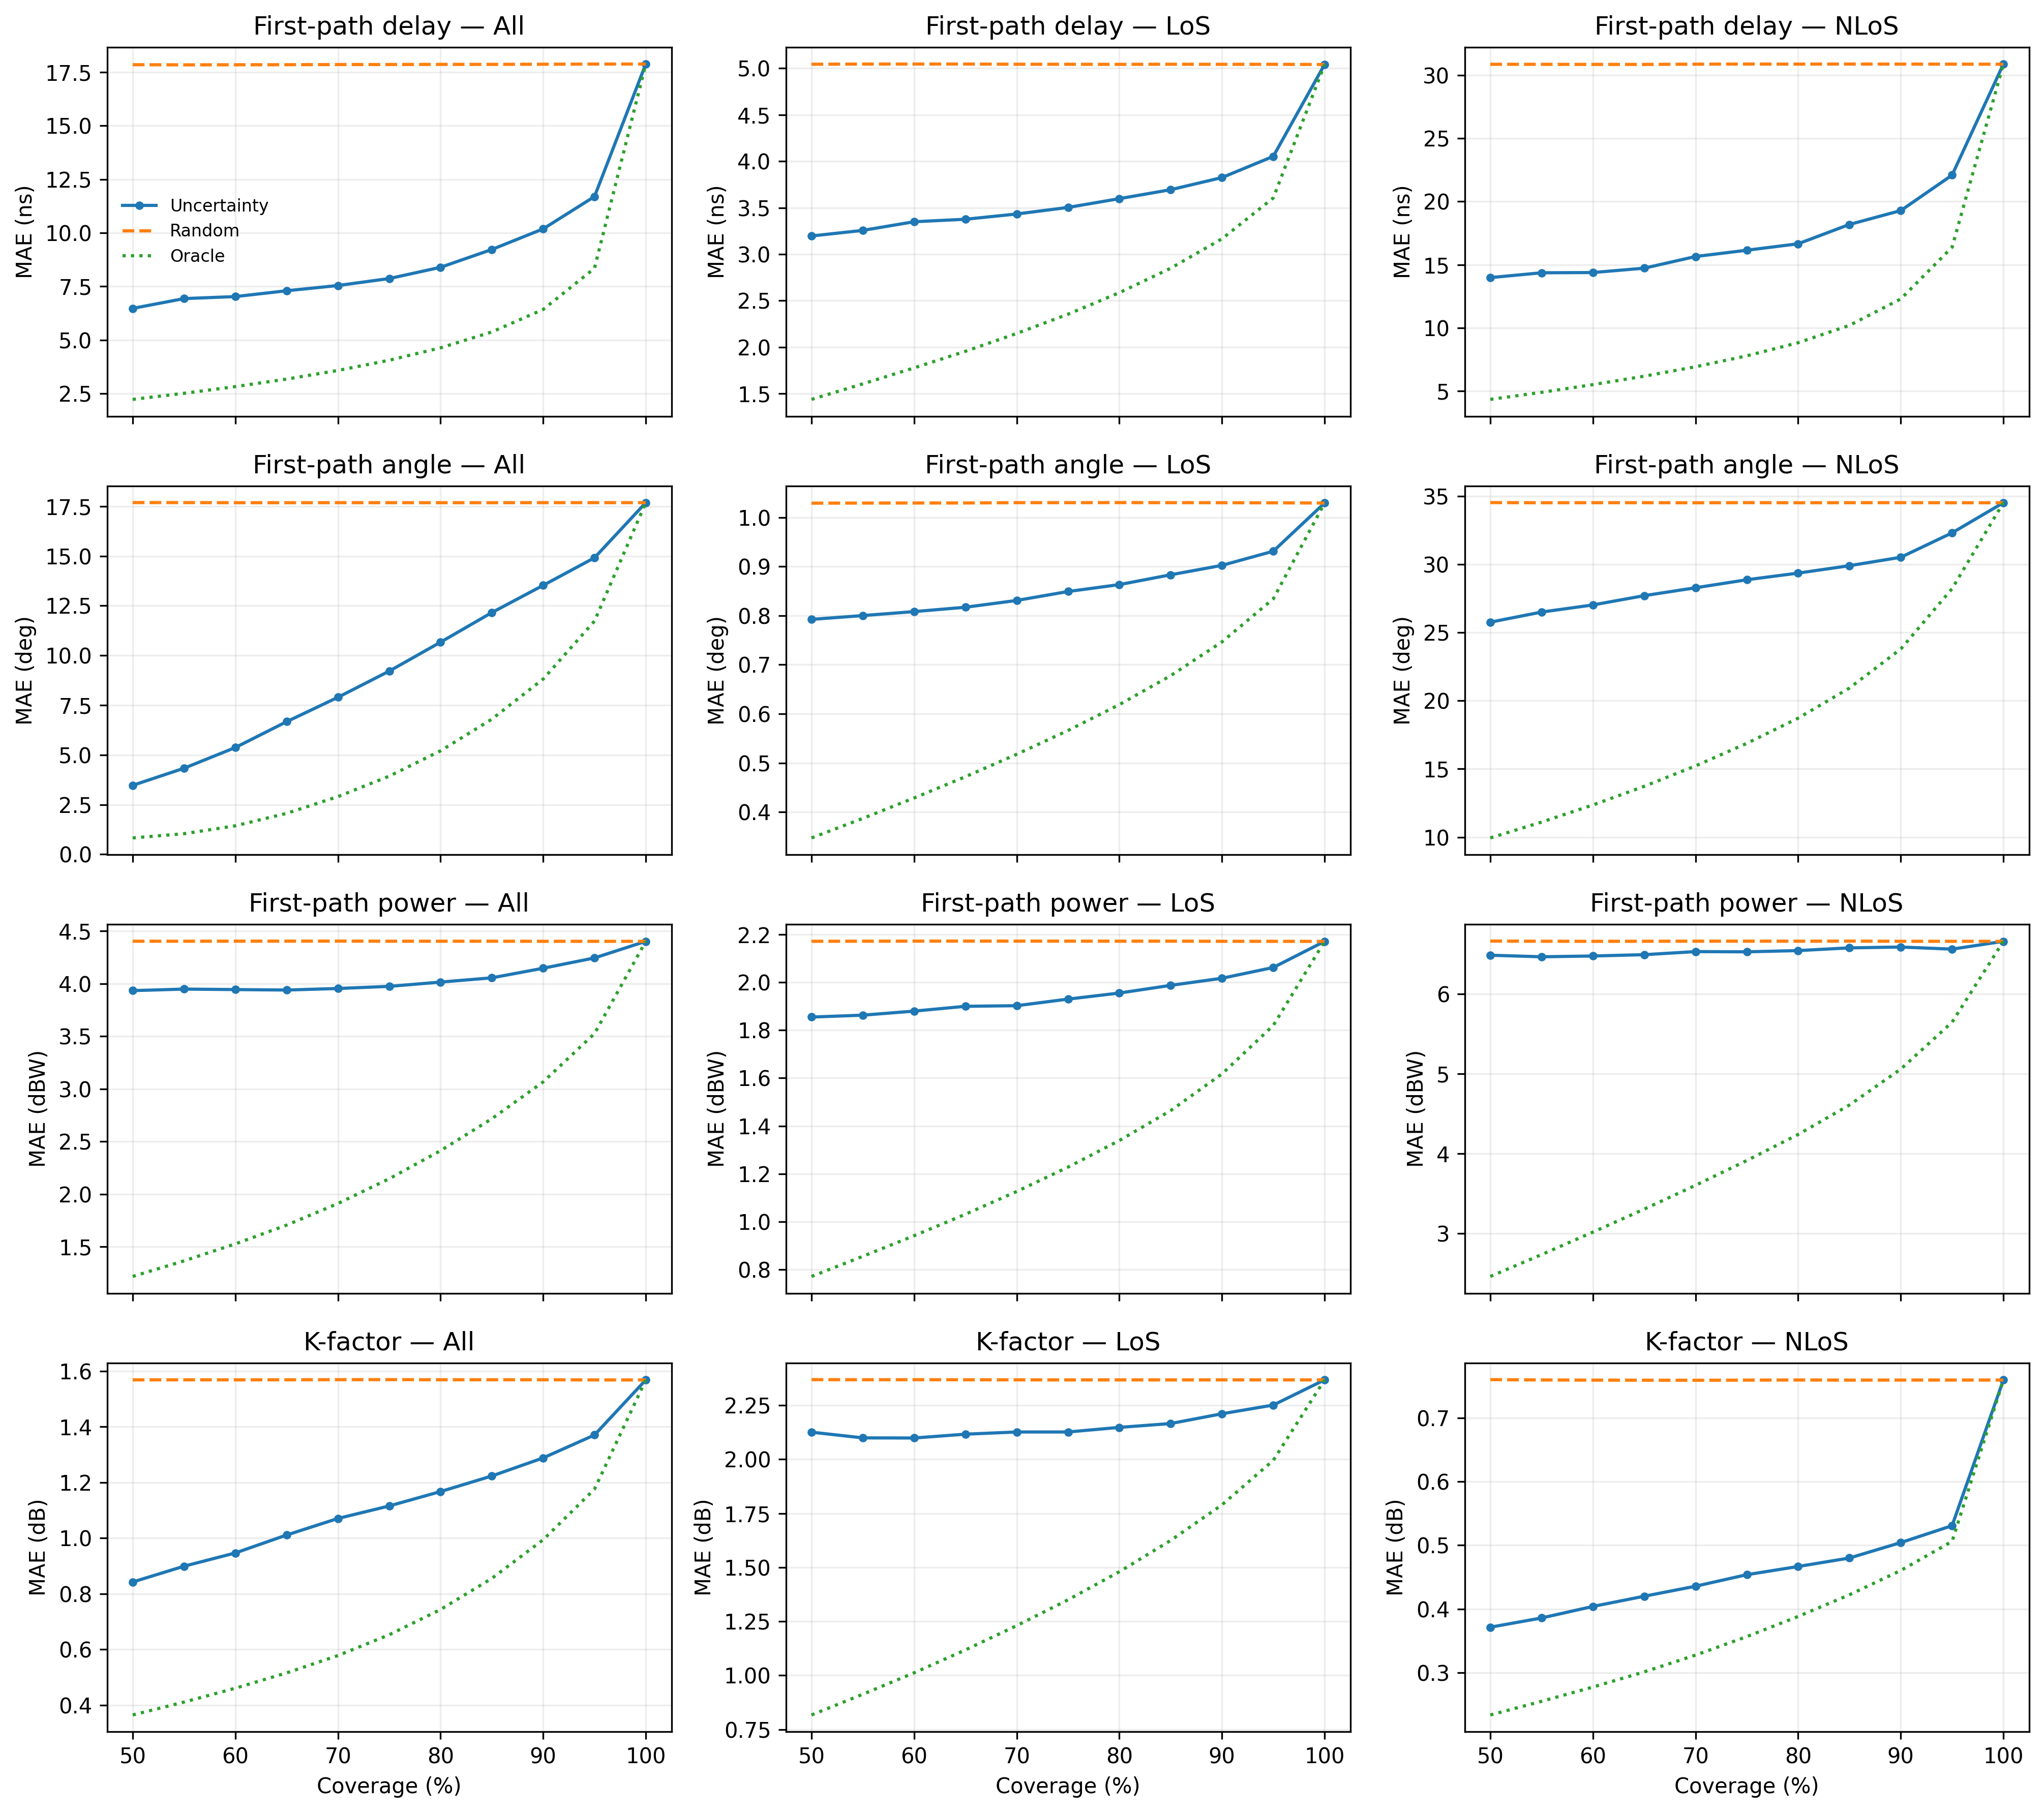
\includegraphics[width=\columnwidth]{figures/risk_coverage_all_metrics.png}
\caption{Risk--coverage curves from the three-seed ensemble for first-path delay, angle, power, and
$K$-factor, evaluated jointly and by LoS/NLoS regime. Blue curves rank samples by ensemble
disagreement, orange lines show random rejection, and green curves give the unattainable oracle
ranking by realized error. Lower coverage means that more high-uncertainty reports are deferred.}
\label{fig:risk-coverage-all}
\end{figure}

Figure~\ref{fig:risk-coverage-all} expands the selective-prediction analysis in
Figure~\ref{fig:nlos-selective-prediction}. Ensemble disagreement is informative for delay and angle:
their MAEs fall steadily as high-uncertainty samples are removed, with the largest absolute benefit in
the NLoS regime. Power is less separable, especially for NLoS, indicating that seed disagreement does
not capture every raw-scale failure. $K$-factor improves more consistently, although its LoS and
NLoS scales differ. The remaining gap to the oracle curves quantifies room for better uncertainty
estimation. These curves support selective deployment rather than replacement of the full-coverage
main metrics: deferred samples require another CSI observation, multi-numerology fusion, or review.

\subsection{Inference Cost}

\begin{table}[t]
\centering
\caption{Physical quality on the inference-cost cohort. Decoder first-delay values can differ from
the learned-baseline table because this benchmark uses a different cohort; model suffixes make this explicit.}
\label{tab:complete-cost}
\scriptsize
\setlength{\tabcolsep}{2.2pt}
\resizebox{\columnwidth}{!}{%
\begin{tabular}{lcccc}
\toprule
\textbf{Method} & \textbf{Delay (ns) $\downarrow$} & \textbf{Angle ($^\circ$) $\downarrow$} &
\textbf{Power (dB) $\downarrow$} & \textbf{$K$ (dB) $\downarrow$} \\
\midrule
\rowcolor{modelblue}\textbf{CSI2TEXT-PGMT-COST-BENCHMARK} & \best{20.68} & $\best{19.55\pm0.38}$ & $5.02\pm0.31$ & $1.87\pm0.24$ \\
\textbf{Single-task} & $47.75\pm5.22$ & $20.65\pm0.32$ & $\best{3.85\pm0.23}$ & $\best{1.42\pm0.04}$ \\
\textbf{PDP/IFFT+MLP} & $27.58\pm5.05$ & $41.62\pm0.68$ & $12.66\pm0.32$ & $5.22\pm0.22$ \\
\textbf{Flattened MLP} & $109.98\pm0.87$ & $34.85\pm0.26$ & $13.06\pm1.17$ & $5.28\pm1.02$ \\
\textbf{Transformer} & $265.91\pm0.02$ & $53.37\pm0.02$ & $38.18\pm0.00$ & $22.52\pm0.00$ \\
\textbf{CNN} & $1619.16\pm1238.13$ & $102.18\pm42.31$ & $14595.56\pm18584.48$ & $55.55\pm34.37$ \\
\textbf{Qwen3-1.7B} & 177.66 & 42.84 & 6.17 & 2.56 \\
\textbf{Qwen3.5-2B} & 162.47 & 42.37 & 5.85 & 2.53 \\
\textbf{DeepSeek-8B} & 232.66 & 59.16 & 27.77 & 16.42 \\
\textbf{InternLM3-8B} & 165.56 & 40.22 & 5.96 & 2.49 \\
\bottomrule
\end{tabular}}
\end{table}

The runtime and memory measurements are consolidated in Table~\ref{tab:inference-cost-main}. Latency is
measured end to end on 200 common examples; quality uses the 1,000-example decoder cohort.
Conventional models use FP32 and direct decoders use 4-bit NF4 weights with BF16
computation. The structured pipeline needs 13.58 ms and 0.13 GB, versus 11--23 s and
1.53--6.18 GB for autoregressive decoders. This is a deployment advantage rather than a replacement
for the physical and text measurements.


For completeness, the original Pareto visualization normalizes each continuous MAE as
\begin{equation}
q_m=\frac{1}{1+\mathrm{MAE}_m/T_m},
\end{equation}
where $T_m$ is the field-specific tolerance. The five shared physical fields are
\[
\mathcal M_A=\{\tau_1,\theta_1,p_1,K,n_{\mathrm{refl}}\}.
\]
For this set,
\begin{equation}
S_{\mathrm{phys}}=100\left(\prod_{m\in\mathcal M_A}q_m\right)^{1/5}.
\end{equation}
For the eight-field continuous set $\mathcal M_C$---first and LoS delay, delay spread, first and LoS
angle, angular spread, first-path power, and $K$ factor---the score is
\begin{equation}
S_{\mathrm{cont}}=100\left(\prod_{m\in\mathcal M_C}q_m\right)^{1/8}.
\end{equation}
The structural and text components are
\begin{align}
S_{\mathrm{struct}}&=100\left(a_{\mathrm{LoS}}a_{\mathrm{path}}a_{\mathrm{refl}}
a_{\mathrm{rpath}}\right)^{1/4},\\
S_{\mathrm{text}}&=100\left(F A_{\mathrm{num}}F_{\mathrm{slot}}(1-H)
A_{\mathrm{delay}}\right)^{1/5},
\end{align}
and the complete score is
\begin{equation}
S_{\mathrm{complete}}=0.50S_{\mathrm{cont}}+0.20S_{\mathrm{struct}}+0.30S_{\mathrm{text}}.
\end{equation}
Here $a_{\mathrm{LoS}}$ averages visibility-state accuracy and macro-F1;
$a_{\mathrm{path}}$ and $a_{\mathrm{rpath}}$ are within-one count accuracies;
$a_{\mathrm{refl}}$ is reflection-bin accuracy; $F$ is factuality; $A_{\mathrm{num}}$ is numerical
tolerance accuracy; $F_{\mathrm{slot}}$ is slot F1; $H$ is hallucination rate; and
$A_{\mathrm{delay}}$ is delay tolerance accuracy. Rule consistency is deliberately excluded.
For CSI2TEXT-PGMT-COST-BENCHMARK, the original visualization gives
$S_{\mathrm{complete}}=78.28\pm0.23$, including
$S_{\mathrm{struct}}=87.34\pm0.18$ and $S_{\mathrm{text}}=94.53\pm0.19$.
Geometric means penalize a single failed field, but the tolerances and the 0.50/0.20/0.30 weights are
design choices that can change rankings. The composite is therefore a visualization aid, not a
replacement for the raw measurements.

\subsection{Reflected-Path Extension}

The main record predicts total reflection-interaction count. A separate head extends the record with
the number of distinct reflected paths. The extension uses RPATH-100K, a naturally imbalanced
100,000-example cohort containing 13,628 LoS and 86,372 NLoS links. Its 80,000/20,000 split contains
10,902/69,098 LoS/NLoS training examples and 2,726/17,274 test examples, so it is not pooled with
the balanced main comparison.

The verbalized reflected-path count reaches MAE $0.091\pm0.007$, RMSE $0.234\pm0.008$, and
within-one accuracy $98.82\pm0.06\%$. Complete descriptions reach
$94.06\pm1.07\%$ factuality, $99.974\pm0.012\%$ numeric-slot F1,
$0.0437\pm0.0200\%$ hallucination, $70.63\pm5.48\%$ numerical tolerance accuracy, and
$99.872\pm0.029\%$ rule consistency. The result demonstrates that total reflection multiplicity and
the number of reflection-bearing paths can be modeled separately. Its strong NLoS skew precludes a
direct numerical comparison with the balanced main cohort.

\section{Qualitative Results, Failure Cases, and Limitations}

\subsection{Representative Channel-Report Templates}

The deterministic verbalizer maps each corrected field to one auditable sentence slot. A LoS report
contains the predicted environment and visibility state, retained path count, first-path delay, angle and
power, delay and angular spreads, $K$ factor, LoS-specific delay and angle, total reflection-interaction
count, and reflected-path count when the extension is enabled. An NLoS report suppresses LoS-only
slots. The corresponding templates are
\begin{align*}
\text{LoS: }&[e,\mathrm{LoS},n_p,\tau_1,\theta_1,p_1,\sigma_\tau,\sigma_\theta,\\[-2pt]
&\qquad K,\tau_{\mathrm{LoS}},\theta_{\mathrm{LoS}},n_{\mathrm{refl}},n_{\mathrm{rpath}}],\\
\text{NLoS: }&[e,\mathrm{NLoS},n_p,\tau_1,\theta_1,p_1,\sigma_\tau,\sigma_\theta,\\[-2pt]
&\qquad K,n_{\mathrm{refl}},n_{\mathrm{rpath}}].
\end{align*}
Qualitative inspection compares every emitted number with the corresponding corrected field rather
than judging surface fluency alone. A reproducible case audit records the sample and cohort ID,
reference record, pre-correction prediction, corrected record, final description, and field-level error.

\subsection{Structured Model Versus Direct Decoder Audits}

The direct decoders usually master the output schema: their slot F1 values are close to those of the
structured model. Their main failure is numerical grounding, especially delay. A useful qualitative
comparison must therefore mark separately: missing slots, unsupported slots, internally inconsistent
values, and values that are syntactically valid but outside physical tolerance. This distinction prevents
perfect rule consistency from being misread as perfect channel prediction.

\subsection{Before and After Relational Correction}

Relational correction operates only on the emitted record. For predicted LoS samples, the earliest-path
and direct-LoS delays are reconciled to the dedicated LoS-delay estimate; negative spreads and invalid
counts are clamped; and at least one retained path is enforced. The raw head outputs remain the proper
measure of neural prediction quality. Before/after examples should therefore display both records and
identify which fields were changed by deterministic rules.

\subsection{LoS and NLoS Failure Cases}

The dominant failure regime is NLoS first-path inference. Direct-path geometry produces stable delay
and angular signatures, while an indirect first retained path is more weakly constrained by the supplied
transmitter-side observation. Failure analysis should be stratified into: incorrect first-path delay,
incorrect receiver-side angle, absolute-power error, reflection-count error, and schema-level error.
The main results show that schema errors are rare relative to physical estimation errors. Future
qualitative panels should sample both typical and high-error cases from fixed cohort IDs rather than
selecting only visually favorable outputs.

\subsection{Scope and Limitations}

All labels and physical relations are derived from finite ray-tracing exports. They inherit the
simulator's path-retention policy, fixed transmit-power assumption, maximum retained-path count, and
reflection encoding. The work establishes a controlled simulator-grounded interface, not field
deployment. Measured-channel validation remains necessary.

The language layer demonstrates auditable realization of a typed record rather than unrestricted
conversation or stylistic generation. Composite factuality is slot based and tolerance dependent; raw
per-field errors must remain visible. Generalization covers selected frequency and array shifts, not
arbitrary bandwidths, carriers, calibration errors, non-Gaussian interference, or hardware
impairments. The AWGN experiment probes one controlled corruption axis only.

The direct decoders have one run each and are not parameter matched, so small ranking differences
are unresolved. Multi-task sharing and language alignment do not improve every target. The robust
conclusion is narrower: target-appropriate representations and structured prediction ground reports
better than direct decoding, while NLoS multipath recovery remains the principal limitation.


\end{document}
